\documentclass{article}
\usepackage[utf8]{inputenc}
\usepackage{float}
\usepackage{graphicx}
\usepackage[a4paper,top=2.5cm,bottom=2.5cm,left=3.5cm,right=3.5cm]{geometry}
\usepackage{wrapfig}
\usepackage{tikz}
\usetikzlibrary{shapes,arrows}

\title{Appunti Advanced Networking \\ and Wireless Systems}
\author{}
\date{aa 2019/20}

\begin{document}

\maketitle

\tableofcontents

\newpage
\section{IPv6}
Gli indirizzi IPv4 stanno finendo a causa della rapida crescita degli utenti Internet (limite teorico di 4.3 miliardi di indirizzi), quindi perchè IPv6 non è ancora lo standard?
\begin{itemize}
    \item Implica un grande cambiamento nell'infrastruttura di rete.
    \item Infrangerebbe un grande principio del protocollo IP: l'\textit{univocità} degli indirizzi.
    \item Il NAT funziona talmente bene nel risolvere problemi di spazio di indirizzamento IPv4 che fino ad oggi non si è sentito il bisogno di passare a IPv6.
\end{itemize}
Tuttavia le cose ora stanno cambiando: la crescita demografica accoppiata ad una crescente richiesta di accesso ad internet (pensiamo a paesi come Cina ed India) si traducono in una grande richiesta di indirizzi IP nel futuro prossimo.
Inoltre, in futuro, con l'avvento dell'IoT ci saranno numerosi oggetti sempre connessi ad internet (es. sensori domestici) per i quali servirà un indirizzo IP permanente (\textit{always-on-access}).

\subsection{IPv6 Base Header}
\begin{figure}[H]
\centering
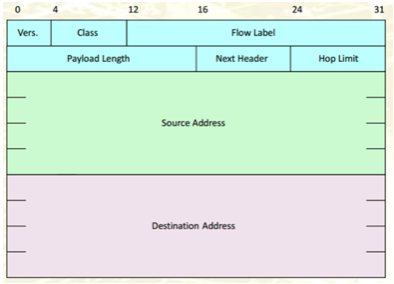
\includegraphics[scale=0.5]{figures/base header.png}
\caption{IPv6 Base Header}
\end{figure}

\begin{itemize}
    \item \textbf{Version} \textit{(4 bits)}: indica che stiamo utilizzando IPv6.
    \item \textbf{Traffic class} \textit{(1 byte)}: sostituisce il campo Type of Service dell’IPv4. Può essere utilizzato per dare priorità a certi a datagram di certe applicazioni (per esempio, pacchetti ICMP) rispetto a datagram di altre applicazioni.
    \item \textbf{Flow label} \textit{(20 bits)}: generato randomicamente. Distingue pacchetti che richiedono stessi trattamenti in modo da facilitare la gestione del traffico real time. E’ considerata una feature sperimentale. Per alcune applicazioni è importante andare a rilevare una sequenza di pacchetti trasmessi da un sender a un receiver. Questo perché i requisiti di un'applicazione possono dipendere da alcune metriche di performance che considerano più pacchetti contemporaneamente. Senza la flow label, per identificare pacchetti appartenenti allo stesso flusso si usavano implicitamente gli indirizzi di destinazione e sorgente. Con questo nuovo parametro si può specificare in modo esplicito. Il sender mette lo stesso valore di flow label per i pacchetti che appartengono allo stesso flow, quindi il flusso viene riconosciuto dai router guardando IP Address del sender e flow label Da aggiungere, inoltre, che con il NAT non funzionava, perché il source address cambia (ci possono essere più sender dietro lo stesso NAT con lo stesso indirizzo).
    \item \textbf{Payload length} \textit{(2 bytes)}: non include la lunghezza dell’header, com’era in IPv4. Gli header di estensione sono considerati come parte del payload.
    \item \textbf{Hop limit} \textit{(1 byte)}: Analogo al campo TTL nell’IPv4, ma in questo caso non è espresso in secondi. Quindi, ogni device intermedio prima della destinazione, riduce di uno l’hop limit, se questo arriva a 0 il pacchetto viene scartato.
    \item \textbf{Next header} \textit{(1 byte)}: Assomiglia al tipo di protocollo in IPv4 ma è molto di più, riflette la nuova organizzazione dei pacchetti IPv6.
\end{itemize}
Nell’header dell’IPv4 c’èra IHL (Internet Leader Length) che serviva per comunicare al ricevitore e ai nodi intermedi la lunghezza dell’header, che era variabile per via del campo options di dimensioni variabili. IPv6, invece ha un header di dimensione fissa, il controllo viene fatto via Hardware. 40 Byte. IPv6 non è provvisto di frammentazione. In IPv4, se il pacchetto è più grande di MTU, si frammenta; in IPv6 si droppa. MTU varia a seconda del canale. 1280 è il minimo MTU che si può assumere su un qualunque link di internet. Se si vuole spedire di più, bisogna stimare MTU lungo il path. 

\newpage
\section{IPv6 Header Structure}
Un Base Header (40 bytes), più zero o più extension headers di dimensione variabile.

\begin{figure}[H]
\centering
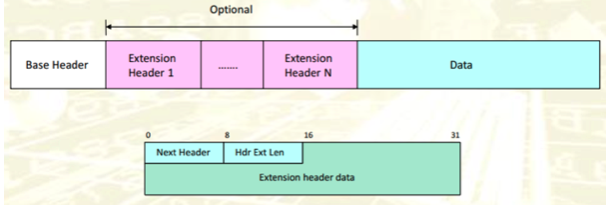
\includegraphics[scale=0.5]{figures/header structure.png}
\caption{IPv6 Header Structure}
\end{figure}

Ogni extension contiene una sola feature e tutti i dati necessari a questa feature.Next header contiene le informazioni sul tipo di dati contenuti nel successivo header. Header extensions length contiene la lunghezza dell’header, in pratica contiene un puntatore alla prossima estensione. \\ Quindi, ogni extension header può essere considerato come un sotto-protocollo che svolge una nuova funzione. E’ possibile che in un extension header sia contenuto un altro pacchetto IPv6: questa tecnica è chiamata “tunneling”. \\ Valori nel campo “Next Header” (base e extension):

\begin{figure}[H]
\centering
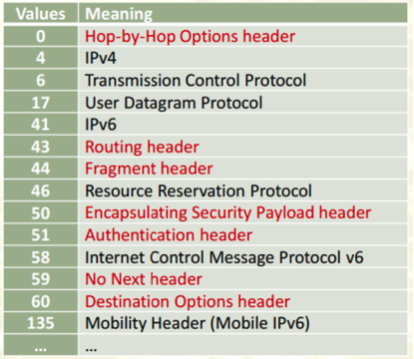
\includegraphics[scale=0.5]{figures/next header values.png}
\caption{IPv6 Next Header Values}
\end{figure}

Gli extension headers vengono inseriti solo quando è necessario. Sono processati nell’ordine in cui appaiono dal nodo identificato dal destination address. \\ Valori che può assumere il campo Next Header:

\begin{figure}[H]
\centering
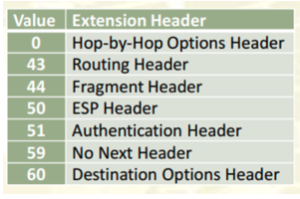
\includegraphics[scale=0.5]{figures/next header used.png}
\caption{IPv6 Next Header Values used}
\end{figure}

I valori “ESP header” e “Authentication Header” servono per sicurezza, autenticazione ed encryption. Valore “No next Header” serve a specificare che non c’è nient’altro nel pacchetto dopo. \\ La regola generale è che il base header venga processato da ogni dispositivo intermedio da cui passa il pacchetto (ogni router del percorso più la destinazione). Mentre gli extension header vengono lette solo a destinazione. L’unica eccezione riguarda l’ “hop by hop options header”.\\ Il “processare un header” si riferisce al fatto che il payload viene mandato al livello superiore. \\ Solitamente si rispetta un ordine, ovvero il “routing header” deve essere prima del “fragment header”.

\subsection{Hop-by-Hop Options header}
Porta informazioni opzionali che devono essere esaminate da ogni nodo sul cammino (hop-by-hop).\\ Se il pacchetto contiene più extension headers, questo deve essere il primo.\\ Formato:

\begin{figure}[H]
\centering
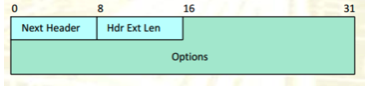
\includegraphics[scale=0.5]{figures/hopbyhop format.png}
\caption{Hop-by-Hop Option Header Format}
\end{figure}

\begin{itemize}
    \item \textbf{Next Header} \textit{(1 byte)}
    \item \textbf{Header Extension Length} \textit{(1 byte)}
    \begin{itemize}
        \item Lunghezza dell’header in unità di otto byte (meno 1)
    \end{itemize}
    \item \textbf{Options}: una o più
\end{itemize}

Per quanto riguarda il campo Options:
\begin{figure}[H]
\centering
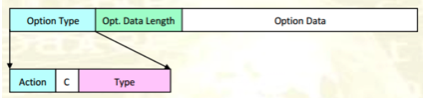
\includegraphics[scale=0.5]{figures/option field.png}
\caption{Option field}
\end{figure}

\begin{itemize}
    \item \textbf{Action} \textit{(2 bits)}: Cosa fare se l'opzione non è riconosciuta
    \begin{itemize}
        \item \textbf{00}: Salta e continua a processare.
        \item \textbf{01}: Scarta il pacchetto.
        \item \textbf{10}: Scarta il pacchetto e manda un messaggio ICMP Parameter Problem all’indirizzo Source del pacchetto.
        \item \textbf{11}: Scarta il pacchetto e manda un messaggio ICMP Parameter Problem all’indirizzo Source del pacchetto solo se la destinazione non è un indirizzo multicast
    \end{itemize}{}
    \item \textbf{C} \textit{(1 bit)}
    \begin{itemize}
        \item \textbf{1}: l’informazione di opzione può cambiare in viaggio
        \item \textbf{0}: l’informazione di opzione non cambia in viaggio
    \end{itemize}
    \item \textbf{Type}
    \begin{itemize}
        \item \textbf{Jumbo Payload} \textit{(Type = 194)}:   Utilizzato per inviare pacchetti molto grandi la cui lunghezza non può essere codificata su soltanto 16 bits (>64 KB). \\ Quando viene utilizzato, il campo length del payload IPv6 è settato a 0. \\ La lunghezza del pacchetto è codificata con 32-bits, supporta la trasmissione di pacchetti che stanno tra 65.536 e 4.294.967.295 bytes (4GB).\\ Compromesso tra il design iniziale di IPv6 e requirements speciali di networking. \\ Quindi, le informazioni del payload non vengono messe all’interno della sezione payload ma all’interno dell’estensione.
        \item \textbf{Router Alert} \textit{(Type = 5)}: Indica ad un router sul cammino di forwarding che il pacchetto contiene informazioni importanti che devono essere processate dal router.\\ Esempio: RSVP utilizza pacchetti di controllo che contengono informazioni che hanno bisogno di essere interpretate o aggiornate da routers sul cammino.
    \end{itemize}
\end{itemize} 

\subsection{Routing Header}
Definisce una lista di nodi intermedi che devono essere visitati sul cammino alla destinazione
\begin{itemize}
    \item \textbf{Routing Type}
    \begin{itemize}
        \item 0: default
        \item 2: Mobile IPv6
        \item 3: RPL
    \end{itemize}
    \item \textbf{Segment Left}: nodi rimanenti che devono essere visitati
    \item \textbf{Address} (RT = 0)
\end{itemize}
Di solito non si ha il controllo sulla rotta utilizzata per raggiungere la destinazione finale. Per avere il controllo sul percorso si usa questa estensione, dove si indica la lista dei router che si vuole che vengano attraversati per consegnare il pacchetto. Non si vanno a rimuovere via via i routers, cosicché il destinatario può sapere il percorso fatto dal pacchetto per raggiungerlo. Non si tiene però conto, in questo modo, del fatto che uno di questi router potrebbe essere congestionato. Soluzione: loose control, ovvero non si specifica tutta la lista ma solo un hop dal quale attraversare. \\ A volte è necessario costruire router senza routing table. Rilevante nelle capillary network dove il router potrebbe essere un sensore. Accade ad esempio in RPL (Routing protocol for low power and lossy network). Un problema è legato al fatto che alcuni nodi intermedi potrebbero essere malevoli e leggere i pacchetti che poi verranno inoltrati. Un altro possibile problema riguarda il DoS attack: ovvero si possono modificare gli indirizzi dei nodi intermedi e far convergere tutto il traffico verso un solo nodo. Per questo motivo adesso questo header è deprecato.

\subsection{Fragment Header}
Diversamente da IPv4, i routers non frammentano pacchetti IPv6.
La frammentazione avviene solo all’host sorgente, che manda il pacchetto. L’host di destinazione gestisce semplicemente il riassamblamento. I pacchetti IPv6 più larghi dell’MTU sul link di forwarding sono scartati dal router. \\
Gli host IPv6 utilizzano una procedura di discovery di cammini MTU.
La minima grandezza IPv6 MTU è 1280 bytes. \\ Questo header viene usato dal sender nel caso voglia frammentare il pacchetto. Solo il sender può usare la frammentazione e il ricevente si preoccupa di ricollegare i pacchetti frammentati. I nodi intermedi non usano frammentazione, inoltrano solo gli stessi pacchetti. \\ Per definizione un link in cui si usa IPv6 deve garantire un minimum MTU pari a 1280 bytes, per cui se un sender manda un pacchetto di dimensione minore a 1280 bytes saprà con certezza che il pacchetto arriverà a destinazione senza essere scartato o frammentato dai router lungo il path. E se un sender volesse mandare pacchetti più grandi di 1280 bytes, deve usare la path MTU discovery per scoprire se lungo il cammino è disponibile un MTU maggiore di 1280 bytes, oppure lo stesso sender può usare la frammentazione. \\ Path MTU discovery procedure: in questa procedura si usa ICMPv6 per scambiarsi informazioni riguardo l’MTU. Per scoprire la minima MTU si manda un pacchetto di una certa dimensione e se non riceviamo in risposta nessun errore ICMPv6, allora l’MTU minimo è sicuramente maggiore della dimensione del pacchetto. Se il minimo MTU è minore, il router scarterà il pacchetto e manderà un pacchetto ICMPv6 di errore al sender con all’interno il valore del minimo MTU.
Se un link non è in grado di garantire una MTU di 1280 bytes, allora non potrà utilizzare IPv6 (sarà un problema con IoT).

\begin{figure}[H]
\centering
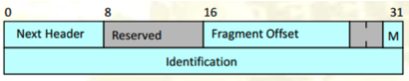
\includegraphics[scale=0.5]{figures/fragment header.png}
\caption{Fragment Header}
\end{figure}

\begin{itemize}
    \item \textbf{Fragment Offset} \textit{(13 bits)}: L’offset in unità di 8 byte del dato in questo pacchetto relativo all’inizio del dato nel pacchetto originale.
    \item \textbf{M-Flag} \textit{(1 bit)}:
    \begin{itemize}
        \item 1: più frammenti
        \item 0: ultimo frammento
    \end{itemize}
    \item \textbf{Identification} \textit{(4 bytes)}: Generato dall’host sorgente in modo da identificare tutti i pacchetti che appartengono al pacchetto originale.
\end{itemize}

\subsection{Altri Extension Headers}
\begin{itemize}
    \item Authentication Header
    \item Encapsulating Payload Security Header \\
    IPv6 security support (IPsec)
    \item No Next Header: No Payload
    \item Destination Options Header \\
    Lo stesso di Hop-by-Hop, ma le opzioni devono essere processate solo alla destinazione. \\
    Utilizzato dal Mobile IPv6
\end{itemize}

\newpage
\section{Categorie di indirizzi IPv6}
Non è presente il broadcast in IPv6. Il broadcast veniva usato in IPv4 con DHCP ad esempio. Il Broadcasting in IPv4 è limitato alla stessa subnet (rete locale, ovvero il router non manda verso l’esterno i pacchetti broadcast). \\
\begin{itemize}
    \item \textbf{Unicast}: identifica in maniera univoca un’interfaccia di un nodo IPv6. Un pacchetto inviato ad un indirizzo unicast è inviato all’interfaccia identificata da quell’indirizzo.
    \item \textbf{Multicast}: identifica un gruppo di interfacce IPv6. Un pacchetto inviato ad un indirizzo multicast è processato da tutti i membri del gruppo multicast.
    \item \textbf{Anycast}: assegnato a interfacce multiple (tipicamente su nodi multipli). Un pacchetto inviato ad un indirizzo anycast è consegnato a soltanto una di queste interfacce (tipicamente la più vicina).
\end{itemize}
In IPv6 si utilizzano di default dei Multicast address per identificare il servizio necessario. Questo indirizzo sarà associato al server che svolge quel servizio, quindi tutti i server DHCP avranno lo stesso indirizzo multicast IPv6. In questo modo il pacchetto viene ricevuto solo dal server DHCP e tutti gli altri nodi non interessati (dato che non forniscono quel servizio) non riceveranno il messaggio, non dovranno quindi processarlo per poi scartarlo (come in IPv4).\\
Un indirizzo IPv6 è assegnato ad un’interfaccia, almeno un indirizzo unicast per interfaccia di un nodo. Una singola interfaccia può essere assegnata a più indirizzi IPv6 di ogni tipo. \\ 
Gli indirizzi IPv6 hanno uno “scope” (codificato come parte dell’indirizzo): lo “scope” è un intervallo topologico tra cui gli indirizzi potrebbero essere usati come identificatori unici. E’ una parte dell’indirizzo che indica la parte della rete dove l’indirizzo può essere usato come unico. Ci sono scope globali e non globali.\\
Non è più presente ARP, il servizio viene fornito direttamente da IPv6. Scope è un sottoinsieme di tutta la network codificata con un indirizzo. In IPv4 c’è solo uno scopo, che è il global-scope, mentre in IPv6 c’è sia il global-scope che local-scope.

\subsection{Link IPv6}
Identificato da un set di interfacce che possono comunicare direttamente tra di loro (hop singolo). Un link IPv6 è un’astrazione, insieme di interfacce che possono comunicare direttamente senza l’intermezzo di un router. Il protocollo IP introduce un modello per modellare la rete. Un link che pensiamo come ad esempio un filo, è in realtà un'astrazione di ciò che il sottostante link-layer protocol permette di fare. Se, per esempio, si dice che un link è broadcast, significa che la sottostante link-layer technology mette a disposizione di IP la comunicazione broadcast (non si parla quindi del mezzo). \\ Ethernet supporta broadcast, la tecnologia però, non lo è. È connessa a degli switch in unicast (point-to-point).
Tipiche assunzioni riguardo ad un link:
\begin{itemize}
    \item Stabile (nel tempo)
    \item Single link-layer broadcast domain
    \item Transitive (se A-B e B-C, allora A-C)
\end{itemize}{}
Implicazioni:
\begin{itemize}
    \item I prefissi network possono essere usati per determinare se un'interfaccia è attaccata ad un certo link.
    \item La rilevazione di indirizzi duplicati può essere facilmente indirizzata
\end{itemize}{}
Se non vale la proprietà transitiva, non si può usare la on-link determination. Quindi, il discorso è che le funzionalità che otteniamo ad un determinato livello (in questo caso 3, IPv6) dipendono da cosa ottieni dai livelli sottostanti.\\ La transitività riguarda i link unicast, non broadcast. Se un link è broadcast puoi far girare una procedura (duplicate address detection - stateless address autoconfiguration) per controllare se ci sono altri nodi sullo stesso link che utilizzano lo stesso indirizzo che si vuole assegnare.

\subsection{Address Scope}
\begin{itemize}
    \item \textbf{Global Address scope}: unico nell'intera internet
    \item \textbf{Link-local}: Assomiglia vagamente ai private address di IPv4, ma è più specifico. Grazie al link-local address ed al fatto che gli host possono autoconfigurare le proprie interfacce, la comunicazione su un link può avvenire senza bisogno di altro, senza bisogno di un gestore.\\
    L'indirizzo quindi è unico sul link al quale è attaccata l'interfaccia corrispondente. 
    \item \textbf{Unique local}: Indirizzo globally unique, ma valido solo in un sottoinsieme dei link. Non dovrebbe essere "routato" nel global Internet.\\ In IPv4 c'erano gli indirizzi privati, come 192.168.0.1: questa soluzione non garantisce unicità globale: collegando 2 reti si hanno conflitti di indirizzi.
\end{itemize}{}

\subsection{Notazione di indirizzi}
\textbf{x:x:x:x:x:x:x:x} dove x è un blocco da 16bit rappresentato da 4 cifre esadecimali.\\ Regole di abbreviazione:
\begin{itemize}
    \item Zeri iniziali possono essere saltati
    \item Zeri consecutivi possono essere sostituiti da "::" e questa regola può essere applicata soltanto una volta, altrimenti non sapresti la dimensione dei blocchi rimossi
\end{itemize}{}
L'indirizzo con tutti 0: \textbf{0:0:0:0:0:0:0:0} (::) indica un indirizzo non specificato.\\ L'indirizzo \textbf{0:0:0:0:0:0:0:1} (::1) indica l'indirizzo loopback, ovvero corrisponde al localhost in IPv4.

\subsection{Prefissi: notazione e allocazione}
Simile all'IPv4 con CIDR: [Indirizzo IPv6]/[lunghezza prefisso].\\
Identifica un set di indirizzi che, ad esempio, possono appartenere alla stessa subnet.

\begin{figure}[H]
\centering
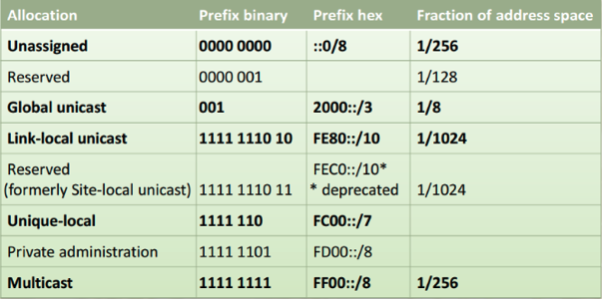
\includegraphics[scale=0.5]{figures/prefix notation.png}
\caption{Allocazione dei prefissi}
\end{figure}

\subsubsection{Global Unicast}

\begin{figure}[H]
\centering
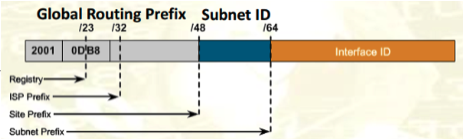
\includegraphics[scale=0.5]{figures/global unicast.png}
\caption{Global unicast address}
\end{figure}

Il prefisso Global Routing identifica il range di indirizzi allocati ad un luogo. Questa divisione è un possibile uso; l'unica cosa obbligatoria è avere una parte per la rete (subnet) e una parte per l'interfaccia. Questo boundary è 64, la divisione è fissata.

\paragraph{Interface ID}
Perché si hanno così tanti bit per l'Interface ID? In IPv4, ad esempio, si hanno $2^{8}-1$ indirizzi assegnabili manualmente o automaticamente, ad esempio tramite un server DHCP. \\ L'idea in IPv6, è fare un'implementazione di questa operazione completamente stateless. Cosa si intende per stateless? E' un pezzo di informazione memorizzato da qualche parte, che sia sul nodo (configurazione manuale) o sul DHCP server. La fai usando il link-layer address. Non c'è uno "state" al livello 3. Il link-layer address è univoco, perché IEEE gestisce lo spazio di indirizzi. È diviso in 2 parti. L'univocità della prima parte in base al produttore, è garantito da IANA, mentre la parte rimanente dipende dal produttore. Si suppone che sia univoco, a livello link-layer. \\ Questa specifica è stata estesa a 64 bit, per questo in IPv6 si usano 64 bit per l'interface ID: tali bit corrisponderanno al link-layer address. \\ Ci sono regole per passare da 48 a 64 bit:

\begin{figure}[H]
\centering
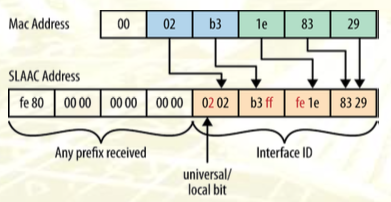
\includegraphics[scale=0.5]{figures/64-48 conversion.png}
\caption{Conversione da 48 a 64}
\end{figure}

\textit{SLAAC = Stateless Address AutoConfiguration} \\ Si aggiungono le parti rosse indicate in figura. Adesso, ogni interfaccia può comunicare il proprio Interface ID. \\ Si crea un problema: si può identificare il dispositivo indipendentemente da dove ti colleghi: per questo, infatti, ci sono diversi modi per generare l'ID dell'interfaccia. 

\subparagraph{Problema della privacy}  
L'accesso ad Internet potrebbe essere tracciato anche tra networks, questo perché l'identificatore è univoco tra le interfacce. 
\begin{itemize}
    \item \textbf{Stable privacy addresses:} Non è basato su un identificatore hardware, viene generato in modo random. Non cambia all'interno di una subnet, ma cambia quando l'host si muove da un network all'altro.
    \item \textbf{Temporary transient:} Assegnato utilizzando un numero random che cambia ad intervalli regolari.
\end{itemize}

\paragraph{Indirizzi link-local e local}
Gli indirizzi link-local sono assegnati di default attraverso auto-configurazione. L'ID Globale di indirizzi univoci IPv6 è generato randomicamente.

\begin{figure}[H]
\centering
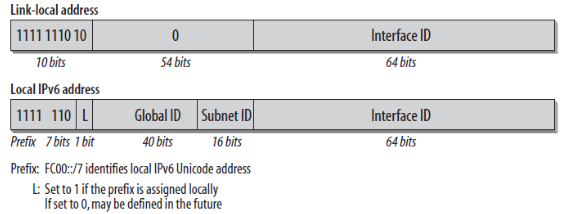
\includegraphics[scale=0.5]{figures/linklocal.png}
\caption{Indirizzi link local}
\end{figure}

I 64 bit finali sono quelli generati nei modi spiegati precedentemente (Interface ID). \\ Prefisso: FC00::/7 identifica gli indirizzi locali IPv7 Unicode. \\ Il bit L è settato a 1 se il prefisso è assegnato localmente e se settato a 0, potrebbe essere definito in futuro.

\subsubsection{Indirizzi Anycast}
Un indirizzo Anycast è assegnato ad interfacce multiple (tipicamente su nodi multipli). Un pacchetto inviato ad un indirizzo anycast è consegnato a soltanto una di queste interfacce (tipicamente la più vicina). \\ Progettato per fornire ridondanza e bilanciamento del carico quando lo stesso servizio è fornito da host o router multipli, come nel caso del DNS. \\ Sappiamo che i nomi in internet hanno una gerarchia ed abbiamo una corrispondente gerarchia di server. Il root server è sempre lo stesso, è un server solo. Servirebbe l'indirizzo dei server, una lista di server; in questo caso si può utilizzare un indirizzo anycast, virtualmente assegnato a tutte le copie del server. Delego alla rete il compito di scegliere il root DNS server giusto. Quindi, il DNS è una routing functionality. \\ Si deve far attraversare ad un pacchetto un autonomous system, se c'è un indirizzo anycast associato con quell'autonomous system, allora sicuramente il pacchetto eventualmente sarà consegnato ad uno dei border router dell'AS. E' implementato come una funzionalità di routing. Per ottenere questo comportamento basta che nella routing table ci sia un'entrata per quello specifico indirizzo. Se è IPv4, significa che si avrà una entry /32 nella tabella di routing: se l'indirizzo di destinazione matcha esattamente questo indirizzo, allora il prossimo hop è questo. Se c'è un'entrata IPv6 /128, questa entrata sarà usata solo come la prima: è il prefisso più lungo che puoi avere. Con questo meccanismo si può quindi andare a stabilire il path che verrà seguito dai pacchetti che fanno match con tale indirizzo. Non c'è bisogno, quindi, di identificare un indirizzo come anycast: un indirizzo anycast è più una funzionalità di routing che un tipo di indirizzo (è l'IP routing che decide dove spedire il pacchetto). Un indirizzo anycast non può essere usato con TCP, dal momento che non c'è controllo sulla consegna, funziona bene con UDP. Il sender quindi, non ha controllo sull'interfaccia al quale il pacchetto sarà spedito. \\ L'indirizzo anycast subnet-router è un indirizzo anycast richiesto:

\begin{figure}[H]
\centering
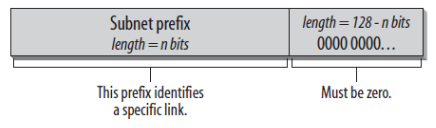
\includegraphics[scale=0.5]{figures/subnet anycast.png}
\caption{Subnet Anycast Address}
\end{figure}

E' associato a tutti i router su una specifica sottorete. Non conosco l'interface ID, altrimenti non sarebbe anycast. Si utilizza ad esempio in Mobile IP.

\subsubsection{Indirizzi Multicast}
Quando un pacchetto è inviato a un indirizzo multicast, tutti i membri del gruppo multicast processano il pacchetto. Un nodo può appartenere a più di un gruppo multicast.

\begin{figure}[H]
\centering
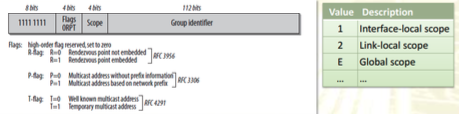
\includegraphics[scale=0.5]{figures/multicast address.png}
\caption{Multicast Address}
\end{figure}

I primi 8 bit sono tutti a 1, poi ci sono 4 bit di flag e 4 bit che indicano lo scope. Non si ha un Interface ID, ma abbiamo un identificativo per un gruppo di interfacce.

\begin{figure}[H]
\centering
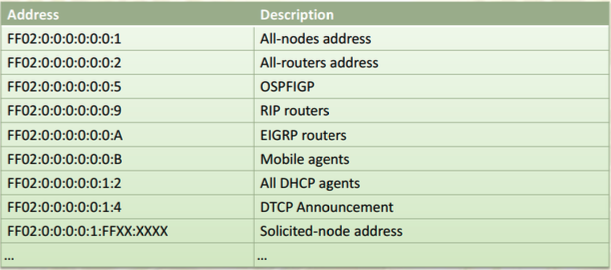
\includegraphics[scale=0.4]{figures/indirizzi tipici multicast.png}
\caption{Indirizzi tipici Multicast}
\end{figure}

\newpage
\section{ICMPv6 e Autoconfigurazione}
In questa sezione ci sono i veri cambiamenti rispetto ad IPv4: molti protocolli che prima erano "satelliti" ora sono parte di IPv6. Un esempio è ARP: non è una traduzione, ma un'operazione di discovery, di lookup. 

\subsection{ICMPv6} 
\paragraph{Internet Control Message Protocol v6}
Basato sulla versione ICMP di IPv4, con le dovute modifiche per adattarsi al nuovo protocollo. Fornisce funzioni diagnostiche e di gestione dell'errore.\\
I messaggi ICMPv6 sono incapsulati in pacchetti IPv6 con il valore \textit{Next Header 58}. Questa nuova versione fornisce anche una nuova funzionalità denominata \textit{Neighbour Discovery Protocol}, che offre procedure per:
\begin{itemize}
    \item Trovare i router.
    \item Risoluzione di indirizzi a livello collegamento (\textit{livello 2}).
    \item Rilevare possibili indirizzi duplicati.
\end{itemize}
Nella versione IPv4 si poteva tener traccia della raggiungibilità dei vicini solo grazie ad ARP.\\ Il protocollo consiste in un set di operazioni:
\begin{itemize}
    \item Router Discovery
    \item Address Resolution
    \item Duplicate Address Detection
\end{itemize}

\subsubsection{Formato del messaggio}
Come già accennato, questo protocollo genera messaggi che sono trasmessi come payload IPv6 con extension number 58, che identifica ICMPv6.
\begin{figure}[H]
\centering
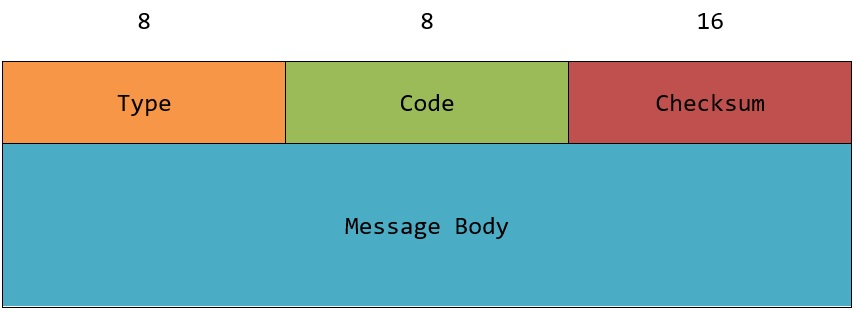
\includegraphics[scale=0.4]{figures/icmp_format.jpg}
\caption{Formato messaggio ICMP}
\end{figure}
Nel messaggio si possono riconoscere i seguenti campi:
\begin{itemize}
    \item \textbf{Type \& Code}:
        \begin{itemize}
            \item Type = 1, Code = 0: Destinazione non raggiungibile. Quindi, quando un router non ha una route per una certa destinazione, manda indietro al trasmettitore questo ICMPv6.
            \item Type = 2: Pacchetto troppo grande. Questo può servire in un protocollo per scoprire il minimo MTU in un path; viene quindi usato nella fase di path MTU discovery e nel body del messaggio viene inserito l'effettivo MTU.
            \item Type = 3: Time exceeded. Viene usato quando scade l'hop counter del pacchetto
            \item Type = 4: Parameter problem. Usato quando un router rileva problemi nel formato del pacchetto.
        \end{itemize}{}
    \item \textbf{Checksum}: Utilizzato per controllare se il messaggio è corrotto. Questi 2 byte sono necessari, dato che IPv6 non ha nessun meccanismo di checksum. ICMPv6 lavora ad un livello più alto di IPv6, quindi ha bisogno del checksum per controllare che il messaggio non sia corrotto.
    \item \textbf{Corpo del messaggio}: Qua ci va l'informazione vera e propria che trasporta il messaggio. 
\end{itemize}
\begin{figure}[H]
\centering
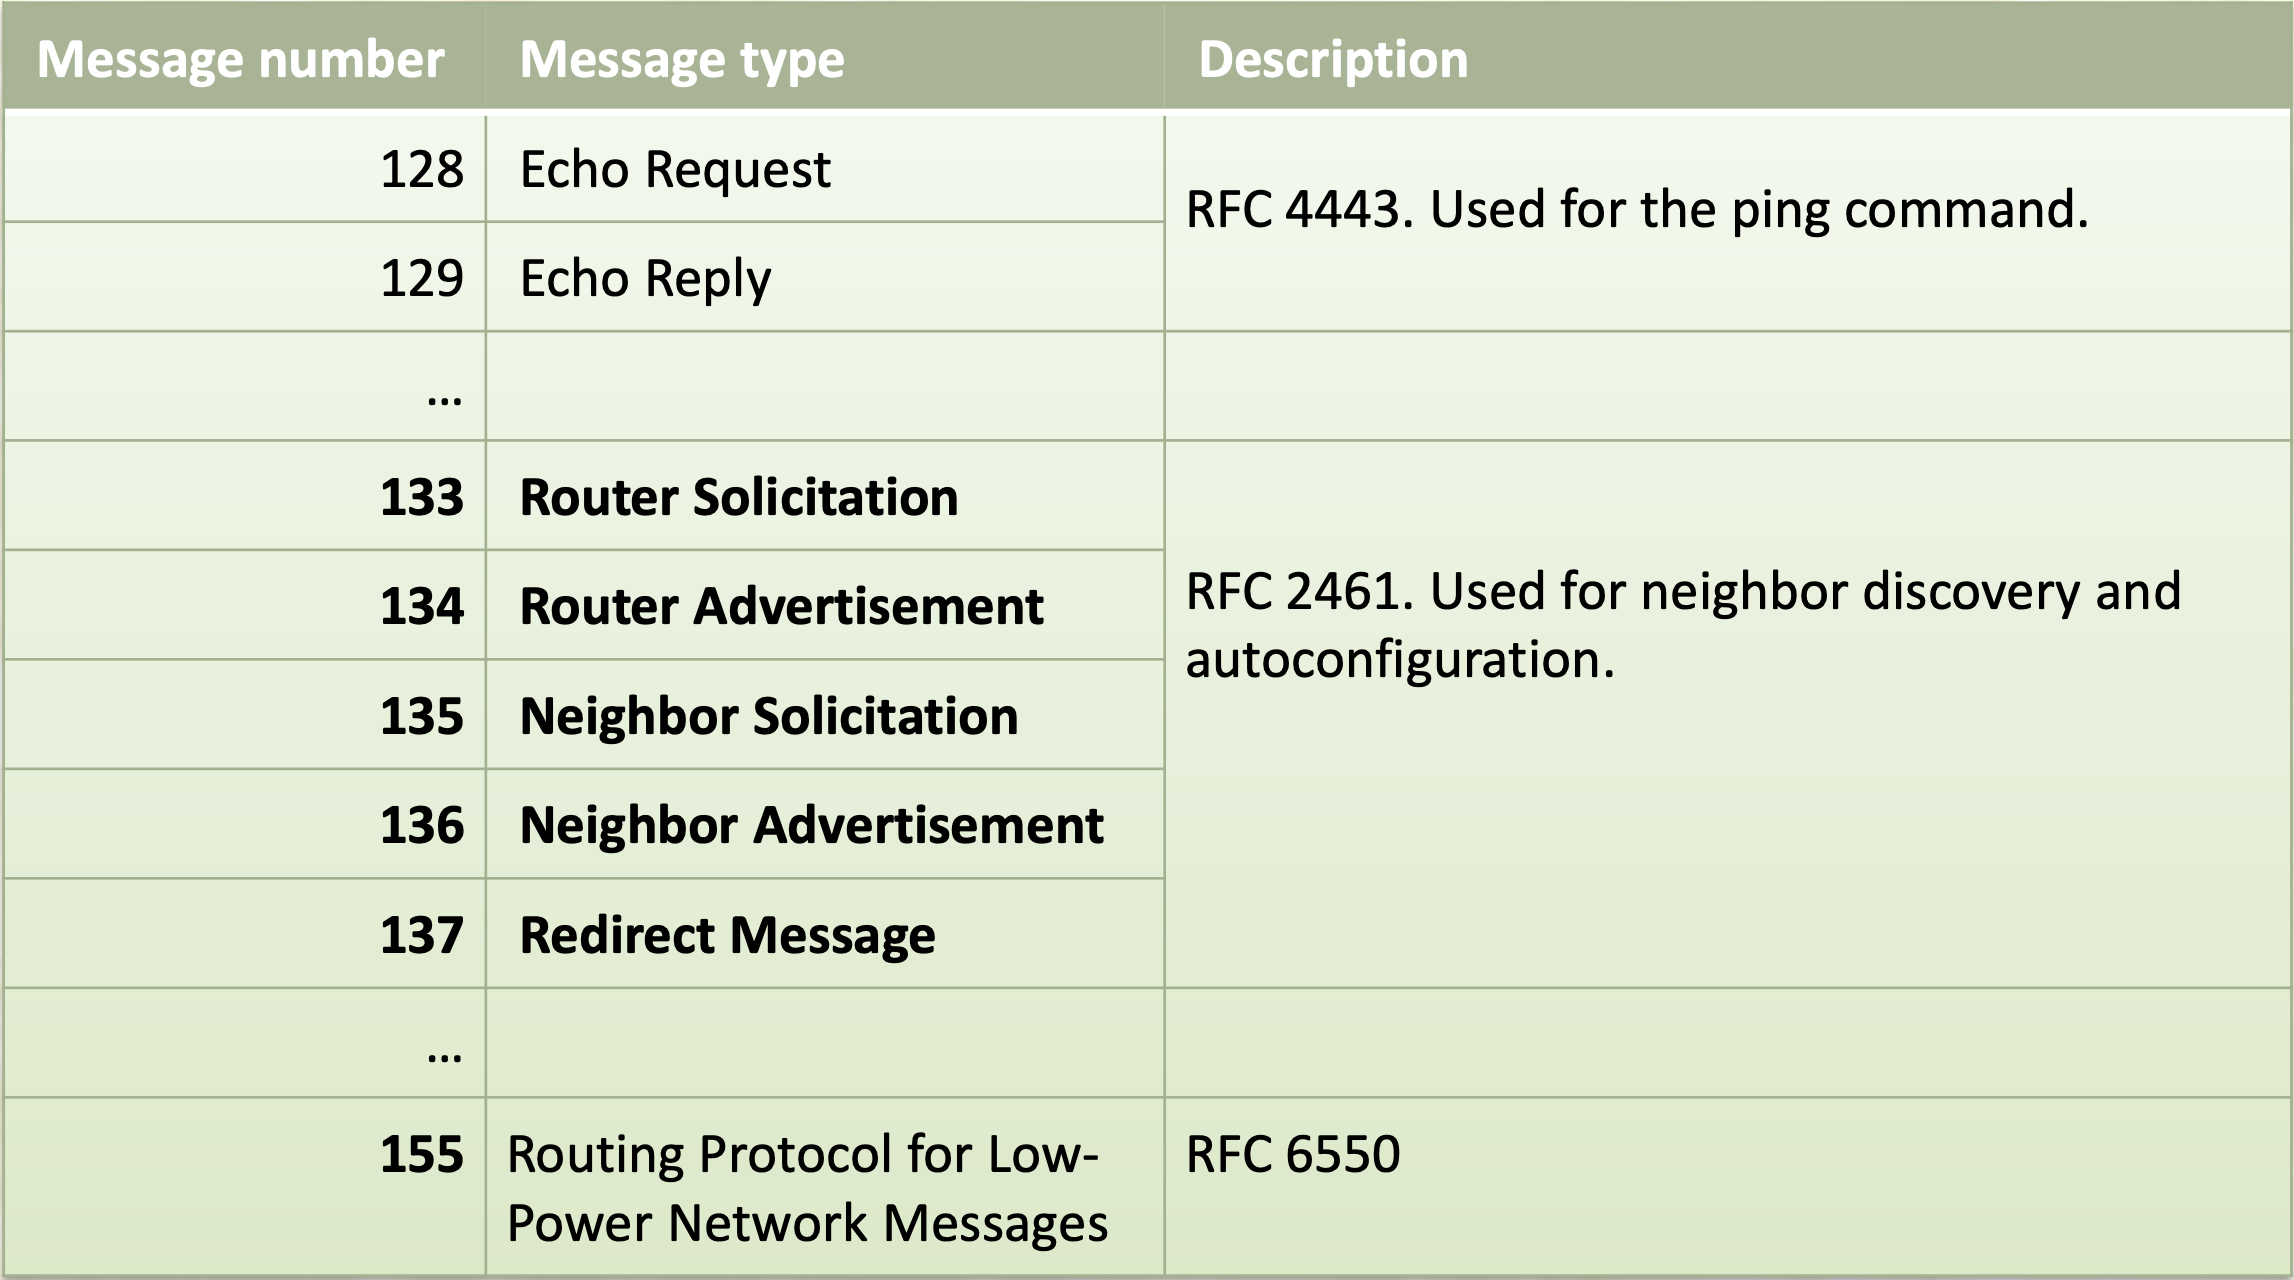
\includegraphics[scale=0.3]{figures/tipi ICMP.png}
\caption{Tipi di messaggio ICMP}
\end{figure}

\subsubsection{Neighbour Discovery protocol}
E' una procedura definita interamente all'interno di ICMPv6 in modo da soddisfare varie feature:
\begin{itemize}
    \item Address Resolution: è un set di funzioni che servono a risolvere un indirizzo IP in un indirizzo layer 2. Sostanzialmente possono verificarsi 2 casi:
    \item Stateless Address Autoconfiguration (SLAAC)
    \item Router Discovery (RD)
    \item Neighbour Unreachability Detection (NUD): per scoprire se qualche vicino non è più raggiungibile
    \item Duplicate Address Detection (DAD)
    \item Redirection
\end{itemize}
Alcune di queste funzionalità sono disponibili anche per IPv4, ma sono implementate in protocolli differenti da IP e ICMP: ad esempio address resolution implementata con ARP. Altre funzionalità, invece, sono nuove come ad esempio SLAAC ed RD.


\subsubsection{Router Discovery}
Periodicamente, i router inviano dei messaggi di \textit{Router Advertisement} all'indirizzo \textit{multicast all nodes} (codice FF02::1). Questi messaggi contengono le informazioni necessarie ad un host che si vuole unire alla rete per autoconfigurarsi sulla stessa. I RA possono essere richiesti esplicitamente da un nodo tramite un messaggio \textit{Router Solicitation}, sempre all'indirizzo multicast (codice FF02::2).
\begin{figure}[H]
\centering
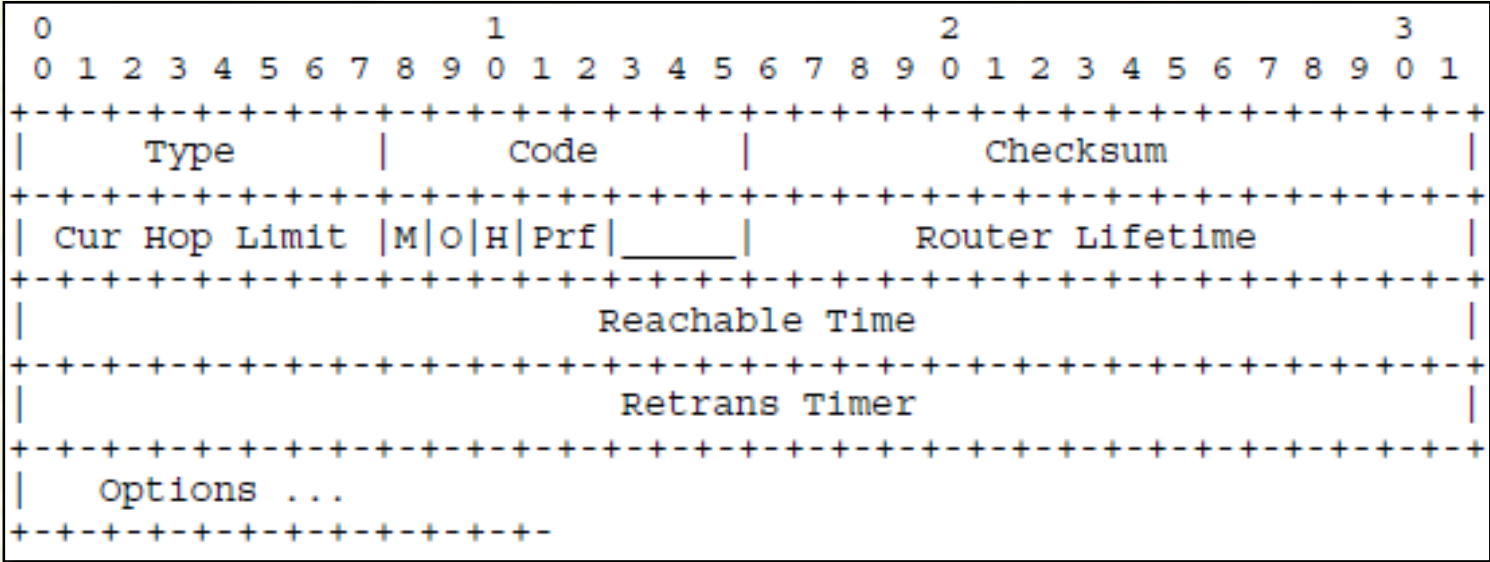
\includegraphics[scale=0.3]{figures/router discovery.png}
\caption{Messaggio router discovery}
\end{figure}
Si vanno ora ad analizzare alcuni campi all'interno del messaggio di Router Advertisement:
\begin{itemize}
    \item Type = 134, Code = 0
    \item \textbf{Cur Ho Limit:} c'è un valore di default per hop limit. Non si può, però, usare un hop limit minore del diametro della nostra rete altrimenti, ovviamente, i pacchetti non arriverebbero al confine. Mentre, non ci sono motivi per impostare un hop limit maggiore del diametro della nostra rete.
    \item \textbf{Time:} parametro di configurazione.
    \item \textbf{M flag:} 
        \begin{itemize}
            \item 0: configurazione stateless: in cui si indica che ci deve essere una configurazione autonoma.
            \item 1: configutazione stateful (DHCP): in questo caso non si può scegliere da soli il proprio indirizzo. Si utilizza il servizio DHCP.
        \end{itemize}
    \item \textbf{Prf flag (2 bits):} Preferenza riguardo al default router. (Gateway in IPv4)
    \item Options
        \begin{itemize}
            \item Source link-layer address
            \item MTU
            \item Prefix information
        \end{itemize}
    \item \textbf{Prefix information option:} informazione relativa al prefix, ce n'è una per ogni prefix. Type e length specificano il tipo e la lunghezza del prefisso. Prefix length è equivalente alla mask in IPv4.
    \item \textbf{L flag:} on-link determination
    \item \textbf{A flag:} se settato, questo flag indica che deve essere eseguito il Duplicate Address Detenction
    \item \textbf{Address lifetime}.
\end{itemize}

\subsection{Configurazione dell'indirizzo}
La configurazione dell'indirizzo può essere fatta in 2 modi, come già accennato precedentemente:
\begin{itemize}
    \item \textbf{Stateful}: DHCPv6
    \item \textbf{Stateless}: Senza nessuna configurazione manuale da parte dell'host. \\ L'interface ID è generato dall'indirizzo MAC (o scelto randomicamente). Il prefisso è imparato dal messaggio di Routing Advertisement.
\end{itemize}
L'indirizzo passa attraverso differenti stati:
\begin{itemize}
    \item \textbf{Tentative Address (provvisorio):} L'unicità in un link deve essere verificata: un'interfaccia scarta pacchetti ricevuti che siano indirizzati ad un indirizzo provvisorio, ma accetta pacchetti di Neighbor Discovery.
    \item \textbf{Preferred Address:} l'utilizzo da parte di protocolli di più alto livello è illimitato.
    \item \textbf{Deprecated Address:} l'utilizzo di questo tipo di indirizzo è sconsigliato ma non proibito.
    \item \textbf{Valid Address:} è un indirizzo che può essere Preferred o Deprecated.
\end{itemize}
Questo tipo di lifetime viene definito in modo da dare il tempo di controllare che non ci siano collisioni sullo stesso link. \\ Si vanno quindi a definire gli step per configurare un indirizzo IPv6:
\begin{itemize}
    \item Si genera un indirizzo link-local appendendo l'identificatore di interfaccia al prefisso del link local \textit{FE80::/10}. L'indirizzo link-local è \textit{tentative}.
    \item Si manda un messaggio Neighbor Solicitation per controllare il Duplicate Address Detection. L'indirizzo link-local diventa \textit{preferred}.
    \item Si manda un messaggio Router Solicitation all'indirizzo "all-routers".
    \item Per ogni prefisso nei Router Advertisement con il flag A settato, viene generato un indirizzo. L'indirizzo è \textit{tentative}, dovrebbe essere utilizzato il Duplicate Address Detection.
    \item L'indirizzo diventa \textit{preferred} fino a che non finisce il lifetime.
\end{itemize}

\newpage
\section{6LoWPAN}
\paragraph{IPv6 over Low-power Wireless Personal Area Networks}
Protocollo progettato per trasportare pacchetti IPv6 nello standard 802.15.4 (\textit{LoW Power Area Networks}) definendo uno strato posto a metà fra il livello 2 ed il livello 3 del modello ISO/OSI.
\begin{figure}[H]
\centering
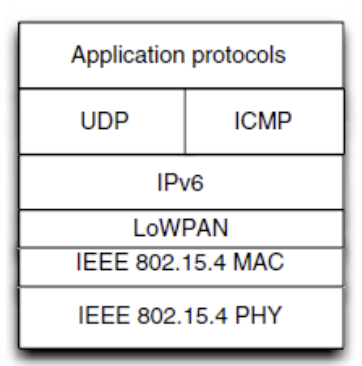
\includegraphics[scale=0.6]{figures/6LoWPAN stack.png}
\caption{6LoWPAN protocol stack}
\end{figure}
Fino ad ora, la ricerca sull'IoT ha implementato protocolli di layer 2 progettati specificatamente per efficienza energetica e nodi vincolati dal punto di vista computazionale. Attualmente, lo standard è 802.15.4, ma ci sono nuove soluzioni che stanno venendo fuori. Come tecnologia su layer 3, le ricerche hanno come obiettivo quello di piazzare IPv6 nello stack IoT, ma questo comporta alcuni problemi. Infatti, IPv6 non è compatibile con 802.15.4. Per superare questo problema, si pone un layer di adattamento nello stack di networking, tra il layer 2 e 3 in modo da fornire compatibilità tra le 2 soluzioni. Questo layer è il \textbf{6LoWPAN}.

\subsection{Architettura 6LoWPAN}
Tipi di nodi in 6LoWPAN:
\begin{itemize}
    \item Hosts 
    \item Routers (6LR)
    \item Border Routers (6LBR): hanno almeno un link attaccato ad una interfaccia fuori dalla 6LoWPAN. Possono essere link punto punto oppure broadcast.
\end{itemize}
I 6LoWPAN sono network detti "stub", ovvero che un tipo di network che non fa passare traffico esterno attraverso essa, tutto il traffico viene generato internamente, a meno che non sia traffico esterno diretto ad un nodo della rete. Le sessioni possono essere iniziate solo da una macchina della rete. \\ Per quanto riguarda la topologia:
\begin{itemize}
    \item Semplice: in cui è presente un solo Border Router.
    \item Extended: in cui sono presenti multipli Border Router. Devono essere connessi allo stesso link fuori dalla 6LoWPAN ed il link deve essere broadcast. Devono quindi poter comunicare fra di loro.
    \item Ad-hoc: non sono presenti Border Router, quindi tutto il traffico è intra-6LoWPAN.
\end{itemize}

\subsection{Multi-hop forwarding in Low Power and Lossy Networks}
Il multi-hop forwarding si può implementare su layer 2 o 3. Nell'implementazione a layer-3 i router sono normali routerIP, se il multi-hop è implementato a layer-2, questo è traparente a 6LoWPAN che quindi non se ne deve curare. Non ci sono limiti alla mobilità dei nodi all'interno della stessa 6LoWPAN, finché un nodo può parlare con almeno un router si può mantenere la comunicazione con qualsiasi altro nodo (senza cambiare indirizzo).\\ Un primo problema da risolvere per ottenere compatibilità tra IPv6 e 802.15.4 è che il primo assume che un subnet è associato ad un singolo link e quindi tutti gli host sullo stesso subnet, possono comunicare fra di loro. Questa assunzione non è sempre vera un network wireless multi-hop. Per esempio, un host A potrebbe comunicare con B, B con C, ma A potrebbe non comunicare direttamente con C perché sono troppo lontani fra di loro. In questo caso, il sottostante modello di link cambia: ovvero, non c'è un singolo dominio broadcast link-layer, ma multipli domini broadcast sovrapposti. In questo tipo di scenario, per ottenere compatibilità con IPv6, un protocollo L2 per network wireless multi-hop, dovrebbe supportare un forwarding multi-hop link-layer, che 802.15.4 non fa. Ci sono quindi due soluzioni per poter ovviare a questo problema: Mesh-Under e Route-Over.

\subsubsection{L2 forwarding (Mesh-Under)}
La soluzione proposta a livello 2 è chiamata "mesh under".\\
Un modo possibile di implementare questo protocollo è il seguente: supponiamo di avere un frame diretto da A a C, ma C non è direttamente raggiungibile. \textit{(Src: A, Dst: C, DATA)}.\\
Si assume, quindi, che C sia raggiungibile tramite un certo B che è raggiungibile anche da A. Quindi, si incapsula il frame in un altro header contenente B come indirizzo di destinazione. \textit{(Src: A, Dst: B, Src: A, Dst: C, DATA)}.\\
Quando B riceve il frame, rimuove il secondo header e controlla il primo, determinando che il pacchetto è rivolto verso C, quindi lo incapsula in un nuovo header e lo manda verso C. \textit{(Src: B, Dst: C, Src: A, Dst: C, DATA)}.\\
Finalmente, C riceve il pacchetto, rimuove l'header e controlla che il pacchetto sia da A verso C e passa i dati al livello superiore.
\begin{figure}[H]
    \centering
    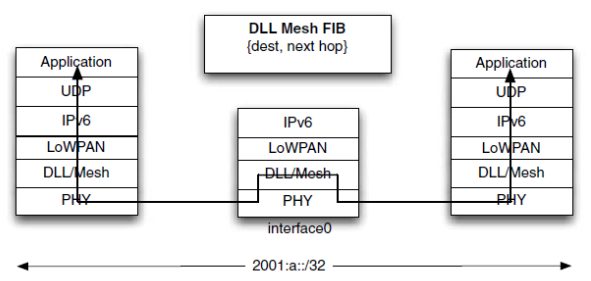
\includegraphics[scale=0.4]{figures/L2 forwarding.png}
    \caption{Mesh Under protocol stack}
\end{figure}
Ovviamente, la scelta del prossimo hop per una certa destinazione, è determinata sulla base di un algoritmo di routing specificato a priori. Si crea un problema che riguarda la mancanza di interoperabilità tra L2 ed L3, quindi la riparazione delle rotte sono lente.

\subsubsection{L2 forwarding vs IP model}
\underline{Definizione di link}: un'area topologica limitata da routers (in cui la comunicazione è regolata da un protocollo L2) che decrementa l'IPv6 Hop Limit quando si fa il forwarding dei pacchetti.\\
\underline{Definizione di subnet}: un'area topologica che utilizza lo stesso prefisso nell'indirizzo, dove quel prefisso non viene ulteriormente suddiviso eccetto per quanto riguarda indirizzi individuali. \\
Nel modello IPv6: una subnet è associata con un link e subnet multiple pootrebbero essere associate allo stesso link. I protocolli L2 dovrebbero essere progettati per realizzare un modello di link consistente con il modello IP. \\
Il modello a cui si deve far riferimento è quello multi-access, in quanto si hanno più nodi che devono accedere allo stesso link, pacchetti mandati ad un indirizzo link-local multicast possono essere ricevuti da tutti i nodi interessati in quel link. Due nodi sul link devono poter comunicare senza nessun decremento dell'Hop Limit dell'IPv6. Deve quindi essere tutto trasparente ad IPv6.
\paragraph{Switched Ethernet}
In Ethernet si ha un esempio di comunicazione cablata multi-hop, fornisce a IP un modello di link multi-access. Viene utilizzato uno spanning tree protocol per implementare un modello multi-access. Questo protocollo opera indipendentemente dalla funzione di forwarding, l'albero creato è un sottoinsieme dei link e questo protocollo viene utilizzato per eliminare loop non graditi. Esiste solo un path per raggiungere la destinazione e viene deciso dal protocollo in fase di creazione. \\ In caso di failure di un nodo, lo spanning tree viene ricreato e ci vogliono pochi secondi per poter ricreare una nuova topologia. Con questo protocollo, si può essere sicuri che gli eventuali messaggi broadcast inviati, arriveranno una sola volta a ogni nodo.
\paragraph{Multi-hop wireless network}
In questo caso, se un nodo trasmette un pacchetto, questa trasmissione sarà ricevuta da tutti i pacchetti nel range della comunicazione, con una sola trasmissione. Quindi in questo caso, a differenza di ethernet, si parla di broadcast medium. Con questa premessa, con broadcast medium, si utilizza una topologia a multicas tree: a differenza di uno spanning tree (che va a coprire tutta la rete), un multicast tree copre solo un sottoinsieme di tutti i nodi della rete, i vari sottoinsiemi di nodi organizzati in multicast tree devono comunicare tra loro per coprire tutta la rete. \\ Si deve considerare in questo caso, che la topologia di rete varia nel tempo in modo impredicibile. I nodi possono essere statici, ma i confini, il range di comunicazione può variare nel tempo a causa di interferenze interne o esterne. \\ Si può implementare facilmente il modello IPv6 (mesh under), ma ci sono alcuni contro in questo caso: le riparazioni a L2 sono lente, in ethernet ci si può accorgere subito di un link malfunzionante tramite controlli elettronici, con la comunicazione wireless questo diventa più difficile e non se ne può accorgere immediatamente, ma dopo un determinato numero di trasmissioni non andato a buon fine. Essendoci una discrepanza da una rete vista a L2 e a L3, si crea un problema in caso di fallimento dei nodi.
\begin{figure}[H]
\centering
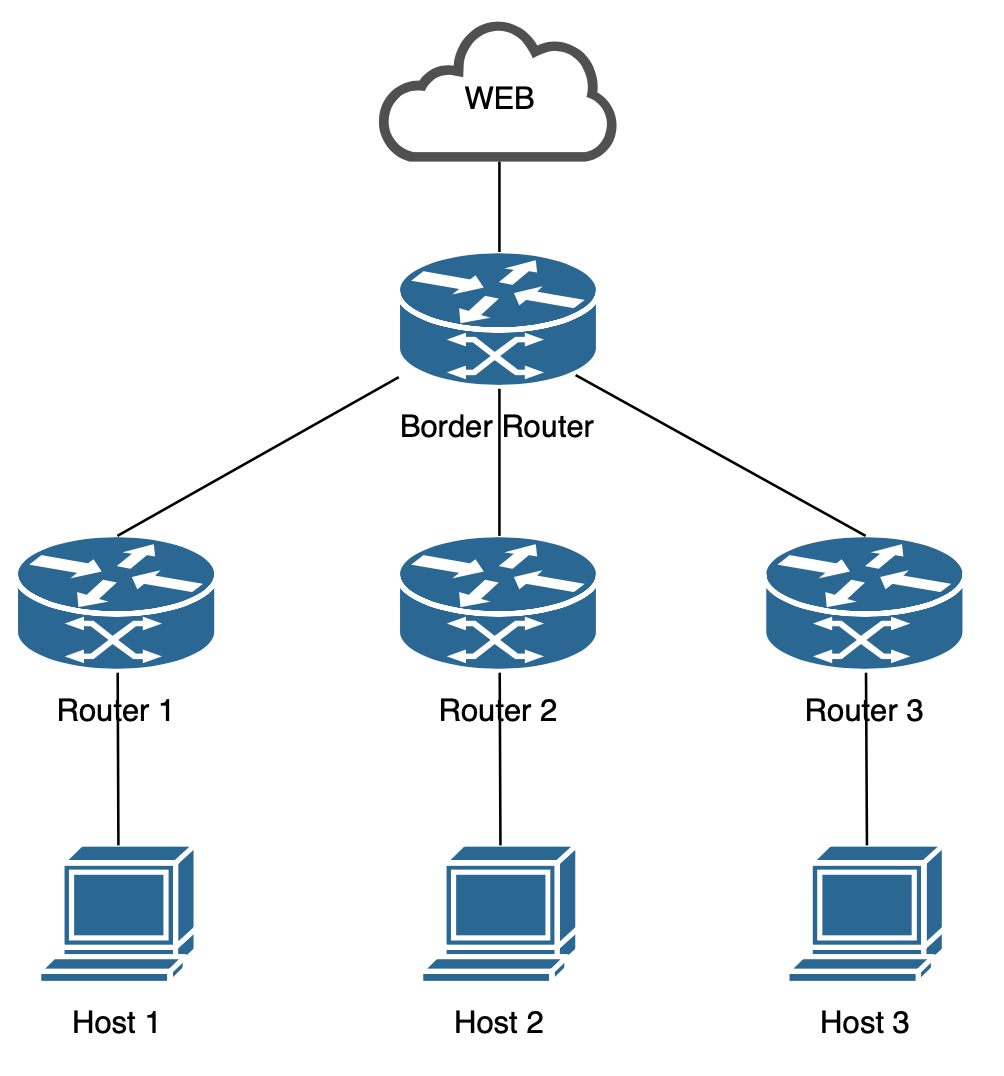
\includegraphics[scale=0.3]{figures/topologia L2.png}
\caption{Topologia a L2}
\end{figure}

\begin{figure}[H]
\centering
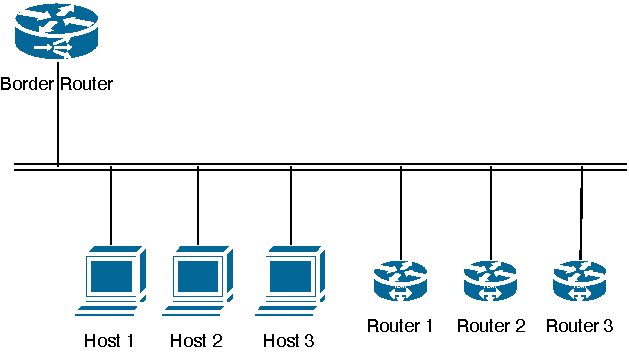
\includegraphics[scale=0.4]{figures/topologia L3.pdf}
\caption{Topologia a L3}
\end{figure}

\subsubsection{L3 forwarding (Route-Over)}
In questo caso, le decisioni di routing vengono prese in base alle informazioni di IPv6, non ci si aspetta supporto dal layer 2. I problemi vengono risolti al layer 3. In 6LoWPAN il routing viene fatto a livello 3, usando delle estensioni per implementare quelle funzioni che IPv6 considera svolte solamente a livello sottostante. Se un pacchetto è frammentato, a ogni router il pacchetto va deframmentato ed analizzato e poi re-frammentato per essere rimandato. Quindi si crea un alto overhead per questo tipo di approccio.
\begin{figure}[H]
\centering
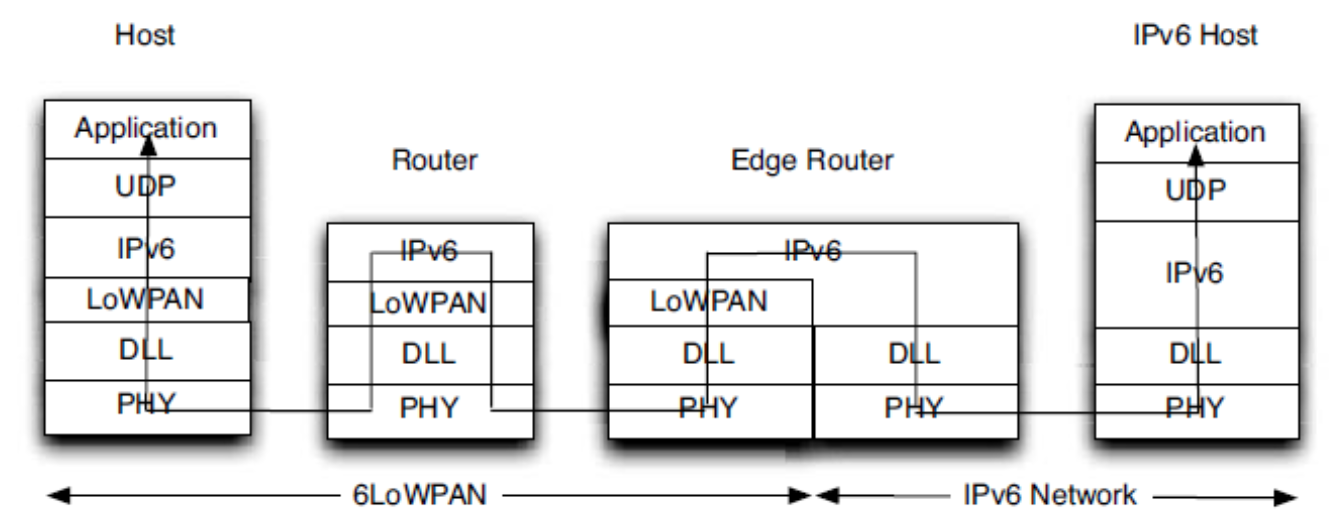
\includegraphics[scale=0.4]{figures/L3 forwarding.png}
\caption{Route-over protocol stack}
\end{figure}

\subsubsection{L3 forwarding vs IP model}
Le domande che vengono poste a questo punto sono: il modello IPv6 funziona? Il modello per cui, una subnet è associata ad un solo link. E poi, qual è il sottostante modello link? Non può essere un modello punto-punto e nemmeno un multi-access, in quanto, nel secondo caso, non ci sarebbe modo di capire cosa si intenda per "stesso link". Un 6LoWPAN è composto da domini di broadcast multipli e sovrapposti. Quindi, l'approccio IP tradizionale non può più essere applicato in questo contesto. 

\subsection{Modello link 6LoWPAN}
In 6LoWPAN non viene fatta nessuna assunzione sul link model (undetermined link model), ogni nodo della subnet condivide lo stesso prefisso. \\ Ogni nodo possiede un link-local scope, che è formato dai nodi che possono comunicare direttamente con esso, ovvero le interfacce che si trovano nel range del segnale radio. In questo modo, nella stessa subnet ci possono essere differenti link-local scope. Quindi, due nodi nella stessa subnet possono condividere lo stesso prefisso, ma avere un link local scope la cui intersezione è nulla. Quindi i nodi nella 6LoWPAN, condividono lo stesso global IPv6 prefix. Questo implica che non si può più utilizzare il prefisso del nodo per inoltrare un pacchetto, perché adesso lo stesso prefisso non significa più stesso link, quindi un nodo con un certo prefisso potrebbe anche non poter raggiungere il nodo destinatario che possiede lo stesso prefisso. Neighbour discovery deve essere esteso e il DHCP non funziona.

\subsection{Addressing}
I prefissi IPv6 sono ottenuti attraverso il Router Advertisements. \\ Gli interface ID IPv6 sono ottenuti in accordo alla procedura \textit{Stateless Address Autoconfiguration (SSA)}. E' obbligatorio avere un mapping tra il link-layer (layer 2) e l'indirizzo IPv6 (layer 3), in questo modo non c'è bisogno di fare address resolution e otteniamo una compressione migliore dell'header. Infatti, l'indirizzo a livello 2 è uguale ad un pezzo dell'indirizzo IPv6. Si ottiene quindi una buona compressione, mettendo tale parte nell'indirizzo.
\begin{figure}[H]
\centering
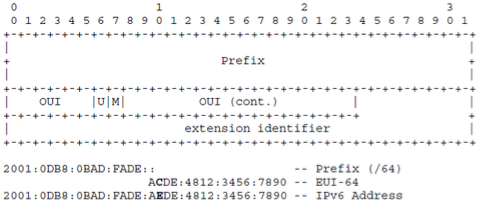
\includegraphics[scale=0.6]{figures/64bit link layer address.png}
\caption{64-bit IEEE EUI-64 link layer address}
\end{figure}
\begin{figure}[H]
\centering
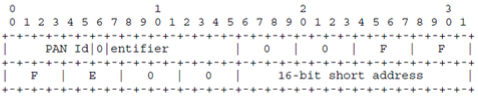
\includegraphics[scale=0.6]{figures/16bit short address.png}
\caption{16-bit short address}
\end{figure}

\subsection{6LoWPAN adaptation layer}
La dimensione di MTU in 802.15.4 è piccola (127 bytes) per far fronte alle limitate capacità dei buffer e per limitare il rate di errori dei pacchetti. \\ Considerando l'overhead del protocollo, nel caso peggiore rimangono solo 81 bytes per il payload. E' necessario quindi un adaptation layer per supportare la frammentazione e il riassemblamento (il minimo MTU di IPv6 è 1280 bytes), implementare la compressione dell'header e ridurre l'overhead del protocollo IPv6. 

\subsubsection{6LoWPAN header stack}
L'header in 6LoWPAN è organizzato come uno stack (come in IPv6), ma con meno flessibilità. Le combinazioni possibili sono ben definite dallo standard:
\begin{figure}[H]
\centering
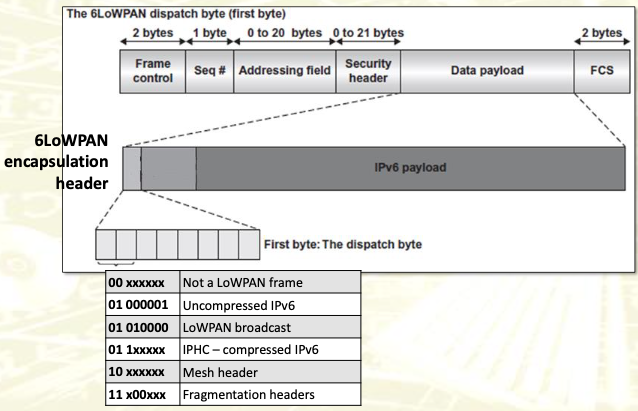
\includegraphics[scale=0.5]{figures/6lowpan header stack.png}
\caption{6LoWPAN header stack}
\end{figure}
\begin{center}
    \textit{FCS: Frame Sequence Check}
\end{center}
Guardando i primi 2 bit si capisce come guardare il resto del payload, in questo modo si definiscono tutte le possibili 8 combinazioni dei bit.
\begin{figure}[H]
\centering
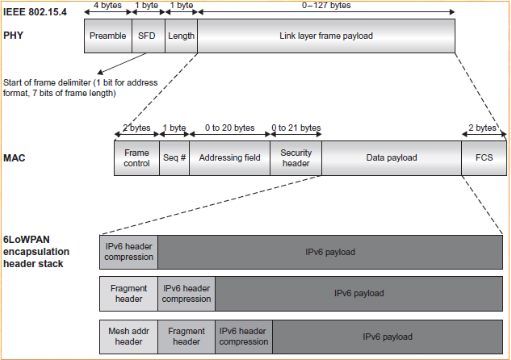
\includegraphics[scale=0.5]{figures/6lowpan header stack 2.png}
\caption{6LoWPAN header stack}
\end{figure}

\subsubsection{Mesh addressing layer}
6LoWPAN supporta il forwarding mesh a livello 2 quando il link-layer utilizza il multi-hop. Ma non è definito nessun protocollo di routing. \textit{Mesh-Under}.
\begin{figure}[H]
\centering
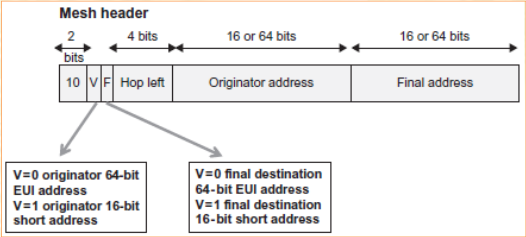
\includegraphics[scale=0.5]{figures/mesh header.png}
\caption{Mesh header}
\end{figure}
Nel caso di broadcast Mesh Under, se non si usa uno spanning tree (e quindi possono verificarsi loop), si ha bisogno di un numero di sequenza che si trova nel link layer, tale che se mandi un pacchetto broadcast con un certo numero di sequenza e lo si riceve con lo stesso numero, lo si scarta. (non è presente la corrispondente immagine per il Broadcast Header)

\subsubsection{Fragment header}
È necessario quando il payload originale IPv6 non può essere trasportato in un singolo frame 802.15.4 perché eccede le dimensioni di MTU.
\begin{figure}[H]
\centering
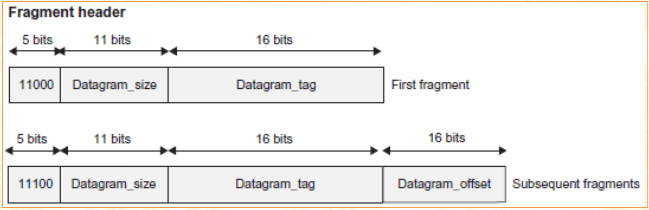
\includegraphics[scale=0.5]{figures/6lowpan fragment header.png}
\caption{Fragment Header}
\end{figure}
Per ogni header successivo al primo, si inserisce l'offset per identificare il frammento relativo al pacchetto originale. \\ La dimensione del datagram è importante in quanto non è detto che i pacchetti arrivino nell'ordine corretto e quindi avere la dimensione del datagram in ogni frammento, consente di allocare memoria qualunque sia il primo pacchetto ricevuto.

\subsubsection{Header compression}
Sono state definite tecniche di compressione IP stateful che si basano sull'ottimizzazione di flow a lunga durata (lifetime). Queste tecniche però, non  ben compatibile con i network 6LoWPAN. In generale, ad esempio in uno streaming video, i pacchetti vanno da una sorgente a una destinazione; in questo caso alcuni campi dell'header vengono mandati tutti insieme (nello stesso flusso). Nel caso attuale, questo approccio non va bene, si vuole una compressione pacchetto-pacchetto ed è sufficiente effettuare una compressione solo nella capillary network, quando il pacchetto arriva al Border Router, non serve più che sia compresso.
\paragraph{Stateless Header Compression}
Nell'header base IPv6, facendo alcune assunzioni, si possono rimuovere alcuni campi.
\begin{figure}[H]
\centering
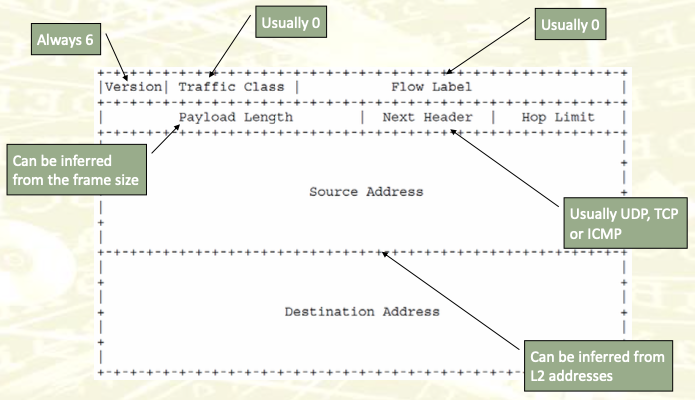
\includegraphics[scale=0.4]{figures/header compression.png}
\caption{Header compression}
\end{figure}
Il tema è che si rimuove e non si trasmettono campi il cui contenuto può essere identificato in qualche modo (ridondanti):
\begin{itemize}
    \item Il campo \textit{Version} è sempre 6.
    \item \textit{Traffic Class} è spesso 0.
    \item \textit{Flow Label} tipicamente non viene considerato.
    \item Il campo \textit{Next Header} è tipicamente UDP, TCP o ICMP.
    \item Il campo \textit{Payload Length} può essere ricavato da il frame di layer 2.
    \item I campi \textit{Source Address} e \textit{Destination Address} possono essere ricavati dal frame di layer 2.
\end{itemize}
Questo approccio stateless, però, non è ritenuto soddisfacente per comunicazioni oltre i link locali, dato che per pacchetti che devono uscire dalla 6LoWPAN, soltanto 8 di 32 bytes possono essere salvati. Questo approccio, quindi, tipicamente non viene usato.
\paragraph{Context-based Header Compression - IPHC}
Si utilizzano contesti condivisi tra source e destination per ottenere una compressione migliore. 6LoWPAN, quindi, sostituisce l'header IPv6 con il seguente header compresso:
\begin{figure}[H]
\centering
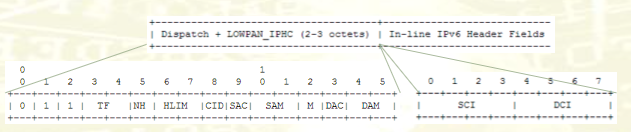
\includegraphics[scale=0.4]{figures/compressed header 6lowpan.png}
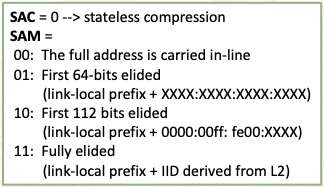
\includegraphics[scale=0.4]{figures/compressed header stateless 6lowpan.png}
\caption{Stateless Header Compression IPHC}
\end{figure}
\begin{figure}[H]
\centering
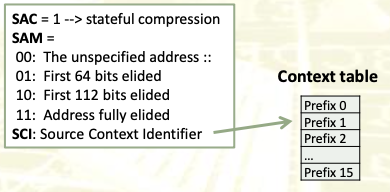
\includegraphics[scale=0.4]{figures/compressed header stateful 6lowpan.png}
\caption{Stateful Header Compression IPHC}
\end{figure}
\begin{itemize}
    \item Il campo \textit{TF} specifica se \textit{Traffic Class} e \textit{Flow Label} hanno valori di default; se non ne hanno i loro valori sono passati come \textit{In-line IPv6 Header Fields}.
    \item \textit{NH} specifica la solita cosa per il campo \textit{Next Header}.
    \item \textit{HLIM} specifica possibili valori per \textit{Hop Limit}
    \item \textit{Source Address Compression (SAC)} specifica quando avviene una compressione statefull o stateless.
    \item \textit{Source Address Mode (SAM)} specifica quanti bit sono stati tolti (elided) e quanti altri sono passati "in-line".
\end{itemize}
In caso di compressione stateful, il prefisso può essere trovato in una tabella di contesto (di 16 entries) condivisa tra il sender e il receiver. Il Border Router diffonde questa informazione nella rete. Occorre semplicemente specificare l'ID del contesto, non l'indirizzo. Si parla, quindi, di stateful perché in diverse 6LoWPAN possiamo avere diverse context table.

\subsection{6LoWPAN Neighbour Discovery (ND)}
La Neighbour Discovery in multicast non è efficiente poiché i nodi potrebbero essere in \textit{standby} per risparmiare energia. Se stiamo usando una \textit{route-over solution} (quindi abbiamo effettivamente più link che si sovrappongono), con la procedura di ND classica posso controllare i duplicati solo all'interno del raggio di trasmissione. \\
Per questo motivo la ND è stata ri-progettata per il 6LoWPAN in modo che ceda della flessibilità in cambio di semplicità. E' stato ridisegnato il modo in cui interagiscono router e host in modo tale che fosse indipendente dal tipo di soluzione adottata (mesh-under o route-over). Qui usiamo un approccio ottimistico: si assume che non ci siano duplicati (quindi non viene eseguito alcun controllo sul DAD - Duplicate Address Detection).
\begin{itemize}
    \item Non si ha broadcast degli advertisement: se vogliamo sapere qualcosa riguardo i nostri vicini dobbiamo inviare un messaggio di \textit{Router Solicitation}.
    \item Un host trasmette un \textit{Router Solicitation} all'indirizzo multicast link-local all-router.
    \item Ciascun router risponde con un messaggio \textit{Router Advertisement} in unicast.
    \item Informazioni utili a tutta la rete 6LoWPAN (prefissi \& info contesto) vengono diffuse (flooding) dal cosiddetto Border Router (6LBR).
\end{itemize}

\subsubsection{Address Configuration}
Lo scambio di messaggi RA e RS avviene tra gli host ed i nodi vicini (entro il raggio di trasmissione). Nella versione originale del Neighbout Discovery ogni router invia periodicamente un RA. In 6LowPAN questo crea troppo overhead,
per cui ogni router invia un RA solo quando riceve un RS message da un host. 
Quindi, si evince che un host invia un RS message per scoprire quali sono i routers nel suo raggio di comunicazione.
Il RA è unicast in modo che l'unico nodo che lo processi sia l'host che ha inviato il RS message. \\
All'avvio, i router si comportano come host per raccogliere la configurazione iniziale, inoltrando i messaggi ai nodi più distanti dal Border Router. Il BR propaga le informazioni (prefissi e context) a tutta la rete. I messaggi che arrivano dal BR possono essere marcati con un'opzione aggiuntiva che serve per indicare il livello di credibilità del messaggio (\textit{Authoritative Border Router Option}). Un messaggio del BR per la configurazione di rete avrà priorità maggiore rispetto alle informazioni salvate sui router. Questo serve per poter correggere eventuali errori sui router.

\subsubsection{Address Registration}
E' un'altra opzione trasportata dai messaggi RS per le reti LLN (low-power lossy networks) che permette di garantire affidabilità e risparmio energetico.\\
Alcuni nodi possono essere mobili quindi, mandano un avviso al router per comunicargli la loro presenza (approccio pro-attivo). Il router mantiene una lista dei nodi che può raggiungere costantemente, con indirizzo a L2 ed L3. In questo modo un router non ha bisogno di verificare la raggiungibilità di un host ogni volta che vuole iniziare una comunicazione. \\
A questo punto è compito del router assicurarsi che non ci siano indirizzi duplicati (DAD). Tuttavia, ci possono essere diversi router (e quindi diverse liste di nodi). Come si può risolvere il problema del DAD in questo caso? Si può risolvere tramite una Tabella DAD centralizzata presso il Border Router. Per supportare questa funzionalità vengono itnrodotti due nuovi messaggi ICMPv6:
\begin{itemize}
    \item Duplicate Address Request (DAR)
    \item Duplicate Address Confirmation (DAC)
\end{itemize}
In questo modo, quando un host vuole registrarsi presso un router, quest'ultimo verificherà presso il BR se l'id dell'interfaccia di rete dell'host è già presente nella Tabella. In caso contrario, procede alla registrazione. \\ 
Nel caso multi-hop, la registrazione avviene attraverso i seguenti passaggi:
\begin{figure}[H]
\centering
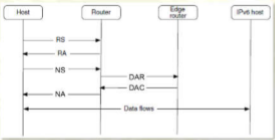
\includegraphics[scale=0.7]{figures/multihop registration.PNG}
\caption{Multi-hop registration}
\end{figure}
Si va quindi a fare una richiesta alla repository per eventuali duplicati, quest'ultima tiene traccia dei nodi nel network. 
\begin{figure}[H]
\centering
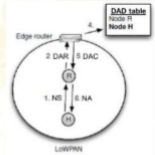
\includegraphics[scale=0.7]{figures/dad table.PNG}
\caption{DAD table}
\end{figure}
Non viene più effettuata la address resolution all'interno dell'host. \\ Per quanto riguarda la trasmissione dei pacchetti:
\begin{itemize}
    \item Indirizzi considerati \textit{on-link}: link-local unicast (prefix fe80::) o multicast (multicast link-local address).
    \item Tutti gli altri prefissi sono considerati \textit{off-link}.
\end{itemize}
Per quanto riguarda la "address resolution": la address registration fornisce supporto per il mantenimento dello stato "host-to-router". La risoluzione per inidirizi basati su multicast non è necessaria.
\newpage

\section{RPL}
Protocollo di routing L3 per le LLNs (low-power lossy networks). Basato sull'algoritmo \textit{Distance-Vector}, introduce alcune ottimizzazioni oltre alla nozione dei vincoli di routing ovvero la possibilità di non considerare solo il percorso a costo minore quando si fa routing ma imporre anche dei vincoli ai percorsi di rete. \\
In questo protocollo supponiamo che i router non si scambino informazioni sullo stato dei link: nessuno ha conoscenza della topologia completa della rete, si conosce indirettamente sapendo la distanza dalle varie destinazioni. \\
RPL costruisce un DODAG (Destination-Oriented Directed Acyclic Graph) ovvero un grafo in cui gli archi sono direzionati ed è privo di cicli. Ciascun nodo ha almeno un arco uscente. \\
Il motivo per il quale si è scelto di implementare un grafo piuttosto che un albero è molto semplice: vogliamo che ci siano più percorsi alternativi verso un determinato nodo. In questo modo si può sopperire ad eventuali malfunzionamenti dei nodi. \\
Nel caso in cui si abbia una rete 6LoWPAN composta da più Border Router (entrambi connessi ad una stessa \textit{backbone} - in questo modo si avrà un unico DODAG virtuale), i nodi vengono divisi in n sottoinsiemi dove n = numero di BR. Ogni nodo può appartenere ad un solo sottoinsieme (DODAG) ed eventuali link che attraversano i sottoinsiemi non saranno più utilizzabili.

\begin{figure}[H]
\centering
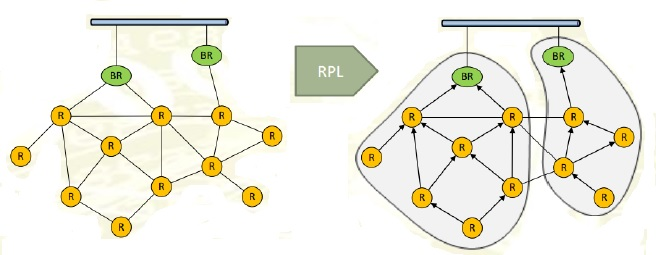
\includegraphics[scale=0.4]{figures/dodag.jpg}
\caption{Multi-sink DODAGs}
\end{figure}
\subsection{Istanze RPL}
In una rete 6LoWPAN si possono avere differenti tipologie di traffico con differenti esigenze/requisiti. Per esempio, ci possono essere messaggi critici che devono essere consegnati il più in fretta possibile in maniera affidabile, oppure messaggi poco utili, che possono anche essere persi o interpolati e, pertanto, devono essere mandati consumando meno energia possibile.
Per questo motivo nella stessa rete possiamo avere differenti istanze di RPL con differenti tabelle di routing. Per ogni istanza RPL quindi, avremo un DODAG distinto che, all'interno della stessa istanza avrà le solite metriche di routing e gli stessi vincoli. Alcuni esempi di vincoli/metriche sui nodi sono:
\begin{itemize}
    \item Stato del nodo e attributi.
    \item Energia (batteria) del nodo.
    \item Numero di hops.
\end{itemize}
Per i link invece avremo:
\begin{itemize}
    \item Throughput.
    \item Latenza.
    \item Affidabilità del link.
    \item Protocollo di routing usato nel link.
\end{itemize}

\subsection{Funzione Obiettivo}
La FO definisce quali metriche/vincoli usare per trovare i percorsi a costo minimo in un'istanza RPL. Per realizzare ciò, i nodi devono conoscere sempre quali sono i suoi genitori (ovvero conoscere la loro posizione all'interno della rete) e il loro \textit{grado/rank} (uno scalare che indica la distanza di un nodo dal BR). Grazie al grado di un nodo, si può sapere se è genitore o figlio di un altro nodo. \\
Il grado di un nodo viene deciso durante la fase di configurazione: il nodo che si vuole attaccare alla DODAG riceve il grado dai nodi a esso vicini; dopo aver scelto tra questi nodi i genitori, il nodo si assicura che il grado scelto sia maggiore di quello dei suoi genitori. Più nel dettaglio:
\begin{itemize}
    \item Il DODAG root inizia ad annunciare la sua presenza inviando messaggi DIO (DODAG Information Object) all'indirizzo link-local multicast.
    \item I nodi RPL ricevono i messaggi DIO e li inoltrano per annunciare a loro volta la loro presenza.
    \item Ricevendo i messaggi DIO, un nodo sa quali sono i nodi vicini a distanza di un hop. Tra questi:
    \begin{itemize}
        \item Determina un set di vicini candidati tra cui scegliere i genitori.
        \item Sceglie un genitore preferito da impostare come percorso predefinito verso il DODAG root.
        \item In base al grado ricevuto dai genitori, il nodo determina il suo grado personale.
    \end{itemize}
\end{itemize}

I messaggi DIO sono periodicamente mandati in broadcast nella rete per mantenere le informazioni di routing aggiornate. La propagazione dei messaggi DIO viene gestita dall'algoritmo \textit{Trickle}.

\subsection{Algoritmo Trickle}
Trickle è un algoritmo di tipo gossip la cui funzione è evitare che la rete sia saturata dai messaggi DIO. Questo viene ottenuto tramite due tecniche:
\begin{itemize}
    \item \textbf{Broadcast Suppression:} vengono selezionati solo alcuni nodi che ritrasmettono, mentre gli altri non possono.
    \item \textbf{Adaptive Periodicity:} modifica la frequenza che indica ogni quanto vengono mandati i messaggi DIO.
\end{itemize}
Ciascun nodo ha un contatore \(\displaystyle c\) ed un timer \(\displaystyle\tau \in [\frac{I}{2}, I]\)
\begin{enumerate}
    \item Inizialmente \(\displaystyle \tau = I\textsubscript{min}\) e aspetto i metadati.
    \item Se i metadati sono consistenti (rispettano le regole dei gradi/rank):
    \begin{enumerate}
        \item \(\displaystyle c++\)
        \item se c $<$ K: il nodo invia i metadati.
        \item quando l'intervallo I scade:
        \begin{enumerate}
            \item \(\displaystyle I = 2I\) fino ad un massimo di \(\displaystyle I\textsubscript{max}\)
            \item \(\displaystyle c=0\)
            \item \(\displaystyle \tau\) = \(\displaystyle \tau' \in [\frac{I}{2}, I]\)
        \end{enumerate}
    \end{enumerate}
    \item altrimenti resetto tutto.
\end{enumerate}
La costante K è detta soglia di ridondanza e indica il numero massimo di messaggi DIO che possono essere ascoltati in un determinato intervallo (misurato da Trickle). Oltre questa soglia si ha la soppressione dei messaggi.

\subsection{Comunicazioni Point-to-Point e Point-to-Multipoint}
Fino ad ora abbiamo considerato solo comunicazioni da nodi verso la radice del DODAG. In RPL è possibile avere comunicazioni \textbf{punto-a-punto} (messaggi dalla radice ai nodi) oppure \textbf{punto-a-multipunto} (da un nodo ad un altro in un altro DODAG). Queste caratterisitiche sono supportate da messaggi speciali chiamati \textbf{DAO - Destination Advertisement Object}, che sono usati dai nodi per avvisare che sono raggiungibili tramite un certo percorso.\\
Esistono due modalità di implementazione:
\paragraph{Storing mode} Assumiamo che i router che compongono il DODAG abbiano abbastanza memoria per memorizzare una tabella di routing.
\begin{enumerate}
    \item Messaggi DAO contengono indirizzo IPv6 del nodo sorgente e sono mandati in unicast verso i nodi "genitori".
    \item Un nodo che riceve un DAO aggiunge un'entrata alla sua tabella di routing che associa l'indirizzo contenuto nel DAO al nodo "figlio" dal quale il messaggio è arrivato. Il nodo "figlio" sarà quindi un \textit{next-hop} per la destinazione specificata nel DAO.
    \item Il DAO viene inoltrato in su per l'albero fino alla radice.
\end{enumerate}
\paragraph{Non-Storing mode} Non avendo memoria a disposizione per la routing table, memorizziamo le stesse informazioni all'interno dei pacchetti.
\begin{enumerate}
    \item Tutti i messaggi DAO convergono alla radice. Ogni messaggio contiene la lista dei nodi attraversati lungo il loro percorso per arrivare alla radice. In questo modo il nodo root conosce tutti i possibili percorsi verso una qualsiasi destinazione.
    \item Il traffico Point-to-Multipoint viene indirizzato dalla root verso il percorso desiderato.
    \item Il traffico Point-to-Point viene mandato al nodo root e poi indirizzato come nel caso P2MP.
\end{enumerate}

\newpage
\section{CoAP}
Constrained Application Protocol, è un protocollo web generico orientato a requisiti specifici (esempio quelli delle LLNs). Il suo scopo principale è quello di realizzare un protocollo applicazione (L5) per servizi web (in comune con HTTP) ma ottimizzato per le applicazioni \textit{Machine-to-Machine (M2M)}.\\
Il livello CoAP è intermedio fra UDP e il livello 5 (applicazione) composto da due sottolivelli: uno gestisce le richieste/risposte, l'altro fornisce il supporto allo scambio di messaggi asincroni. I messaggi asincroni servono per poter inviare un messaggio al client anche quando questo non ha effettuato alcuna richiesta (non è possibile in TCP).\\
\begin{figure}[H]
\centering
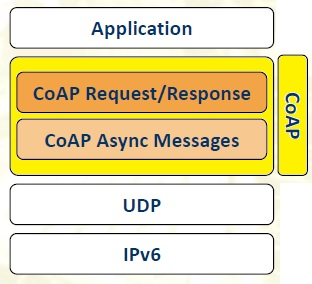
\includegraphics[scale=0.4]{figures/coaplayer.jpg}
\caption{Posizione del livello CoAP}
\end{figure}
CoAP utilizza un modello di interazione Request/Response (simile ad HTTP) asincrona, con alcune opzioni per l'affidabilità. Una trasmissione non-affidabile viene iniziata dal mittente che invia un messaggio NON al quale non riceverà risposta. Una trasmissione affidabile invece, viene iniziata tramite l'invio di un messaggio CON. Il ricevente può:
\begin{itemize}
    \item Rispondere con ACK oppure
    \item Rifiutare con RST.
\end{itemize}
Il mittente ripete il messaggio CON finchè non riceve ACK o RST oppure finchè non scade un timeout (solitamente 2 secondi).

\paragraph{Modello Request/Response} Modello simile all'HTTP. Una richiesta include un metodo, l'URI di una risorsa e, opzionalmente, metadati (opzioni CoAP). I possibili metodi per una CoAP Request sono:
\begin{itemize}
    \item GET: richiede una rappresentazione dello stato di una risorsa.
    \item POST: creazione di una risorsa.
    \item DELETE: richiede la cancellazione di una risorsa.
    \item PUT: creazione o aggiornamento di una risorsa.
\end{itemize}
Le CoAP Response contengono un codice, il payload e, al solito, meta-dati opzionali. La corrispondenza tra Richieste-Risposte è garantita mediante l'utilizzo di un token. Le possibili classi di codici di risposta sono:
\begin{itemize}
    \item Successo (codice 2.xx)
    \item Client-error (codice 4.xx)
    \item Server-error (codice 5.xx): il server è consapevole di aver sbagliato oppure è impossibilitato ad eseguire la richiesta ricevuta.
\end{itemize}

\paragraph{CoAP Proxy} Potremmo voler implementare un intermediario (proxy) che si pone fra i client ed i server il cui compito principale sarebbe quello di inoltrare richieste/risposte ai destinatari. Un Proxy CoAP potrebbe anche svolgere funzioni di \textit{caching}, traduzione protocolli oppure traduzioni nomi. \\
Nel caso della traduzione protocolli si ha un Cross-Protocol Proxy (o Cross-Proxy).

\subsection{Resource Observing}
Client e Server si scambiano la rappresentazione (stati) delle risorse grazie ad un modello publish/subscribe. Un Client interessato a ricevere aggiornamenti su una risorsa si "iscrive" (observe) presso il server che gestisce quella risorsa. L'approccio è di tipo \textit{best-effort}. Definiamo alcuni termini:
\begin{itemize}
    \item Soggetto: una risorsa su un CoAP server.
    \item Observer: un CoAP client.
    \item Registrazione: una richiesta GET \textit{estesa}.
    \item Notifica: una risposta CoAP aggiuntiva inviata ai client registrati ogni qualvolta lo stato di una risorsa cambia.
\end{itemize}

\newpage
\section{QoS - Quality of Service}
Vogliamo gestire il modo in cui i pacchetti viaggiano nella rete. In particolare, dobbiamo considerare che alcuni pacchetti devono essere trattati in maniera diversa da altri. Questo perché esistono diverse tipologie di applicazioni con requisiti diversi (es. real-time e non).

\subsection{Algoritmi QoS}
Le proprietà desiderabili di un algoritmo QoS sono:
\paragraph{Isolamento dei flussi} L'algoritmo deve essere in grado di isolare un flusso dagli effetti indesiderati degli altri. Idealmente, l'algoritmo dovrebbe fornire al flusso un link dedicato con capacità uguale al rate minimo garantito per quel flusso. In questo modo, le prestazioni di un flusso non sono influenzate dalla presenza di altri flussi.\\
\paragraph{\textit{Fairness}} La capacità di un link dovrebbe essere divisa fra i flussi richiedenti in maniera equa. A questo scopo si definisce l'Indice di Jain.\\
\underline{Ipotesi}: se fair share = equal share e tutti i percorsi hanno la stessa lunghezza, allora l'Indice di Jain \( \in [0, 1]\) è così definito:\\
\[ f(x\textsubscript{1},...,x\textsubscript{n}) = \frac{(\sum_{i=1}^n x\textsubscript{i})\textsuperscript{2}}{n\sum_{i=1}^n x\textsubscript{i}\textsuperscript{2}}
\]
dove \(\displaystyle x\textsubscript{i} \) è il \textit{throughput} del flusso i.\\
Se invece come definizione di fairness scegliamo di allocare la massima capacità disponibile di un link ad un flusso, avremo la \textbf{Max-Min fairness}. In questo modello si alloca ad un flusso la massima capacità disponibile di un link ovvero \( \displaystyle \phi\textsubscript{i} = \frac{c}{n} \) dove n è il numero di flussi che attraversano quel percorso.
\begin{figure}[H]
    \centering
    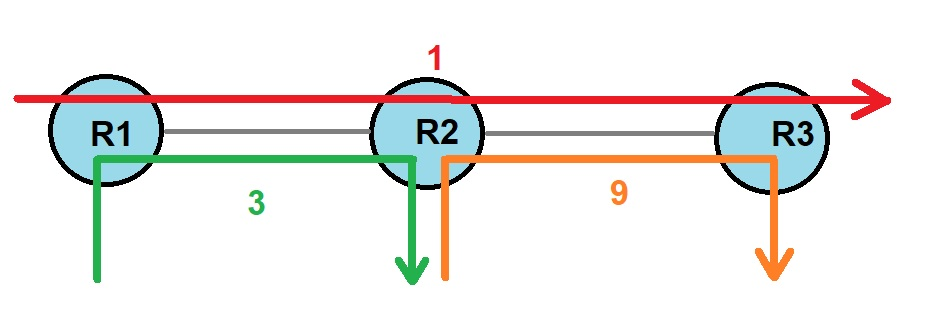
\includegraphics[scale=0.4]{figures/maxmin.jpg}
    \caption{Max-Min fairness}
\end{figure}
Supponiamo, per esempio, di avere tre percorsi attraverso tre router come mostrato in figura. Avremo un set 0 composto da 1 flusso che attraversa tutti i router, un set 1 composto da 3 flussi che attraversano R1 ed R2 ed infine un set 2 composto da 9 flussi che attraversano R2 ed R3. Quindi tra R1-R2 abbiamo 3+1=4 flussi mentre tra R2-R3 abbiamo 1+9 = 10 flussi.\\
Segue che \(\displaystyle \phi\textsubscript{1} = \frac{c}{4}, \phi\textsubscript{2} = \frac{c}{10}\) mentre \(\displaystyle \phi\textsubscript{0} = min(\phi\textsubscript{1}, \phi\textsubscript{2})\). Questo petche il set 0 attraversa tutti i router e quindi la sua porzione di banda allocata sarà la più piccola fra le disponibili. In questo caso si dice che \(\displaystyle \phi\textsubscript{2} \) è un \textit{bottleneck} per \(\displaystyle \phi\textsubscript{0} \).\\
Non sempre una divisione in parti uguali è \textit{fair}. Nell'esempio precedente, il set 0 sfrutta una capacità di 0.1c sul link R1-R2 a fronte di una capacità allocata di 0.25c. In questo modo, il set 1 si trova con una capacità totale di 0.75c (anziché 0.9c). Per ottimizzare questa allocazione si può usare un algoritmo noto come \textit{Progressive Filling}.\\
L'algoritmo Progressive Filling prevede che inizialmente tutti i set abbiano \(\phi\textsubscript{i}=0\). Dopodiché, vengono tutti incrementati della stessa quantità finché non si raggiunge la saturazione di un link. A questo punto, tutte le bande allocate ai flussi che attraversano il link saturo vengono fissate. Si procede dunque all'incremento dei rimanenti set finché tutti i link non sono saturi.\\
Applicando il Progressive Filling all'esempio precedente si ottiene \( \phi\textsubscript{0}, \phi\textsubscript{2} = \frac{c}{10} \) e \( \phi\textsubscript{1} = \frac{1}{3}(c - \frac{c}{10}) = 0.3c\)\\ \\
Si può avere inoltre la \textbf{Proportional Fairness} quando la capacità del link viene allocata ad un flusso in base alla richiesta di capacità dello stesso.\\ \\
DEFINIZIONE di Flusso \textit{backlogged}: Data A(t) funzione di input ad un server e W(t) funzione di output del server, la funzione Q(t) = A(t) - W(t) è definita backlog e rappresenta il lavoro incompleto (lunghezza della coda nel buffer). D'ora in avanti i flussi \textit{backlogged} saranno definiti arretrati.\\ \\
Un altro indice di fairness è l'Indice di Golestani, noto più semplicemente come \textit{Service Fairness Index}, definisce la massima differenza tra il servizio normalizzato ricevuto da due flussi arretrati, su un intervallo in cui entrambi sono continuamente arretrati.\\
\[
    RF\textsubscript{(i,j)}(t\textsubscript{1}, t\textsubscript{2}) = | \frac{W\textsubscript{i}\textsuperscript{S}(t\textsubscript{1}, t\textsubscript{2})}{t\textsubscript{i}} - \frac{W\textsubscript{j}\textsuperscript{S}(t\textsubscript{1}, t\textsubscript{2})}{t\textsubscript{j}} |
\]
dove \( W\textsubscript{i}\textsuperscript{S}(t\textsubscript{1}, t\textsubscript{2}) \) denota il servizio ricevuto dal flusso i misurato in unità di traffico (bit), nell'intervallo \( (t\textsubscript{1}, t\textsubscript{2}) \), sotto la disciplina di scheduling S.

\paragraph{Garanzie sul Ritardo end-to-end} Il tempo di ritardo di un pacchetto su una rete può essere visto come una variabile aleatoria. Possiamo quindi caratterizzare il ritardo in due modi:
\begin{itemize}
    \item Deterministico: vincolato al ritardo, variazione ritardo.
    \item Probabilistico: media, percentili ecc.
\end{itemize}

\paragraph{Piena Utilizzazione}
\paragraph{Semplicità} Infine, bisogna considerare la semplicità di implementazione. Vogliamo che, alla peggio, l'algoritmo di selezione del pacchetto abbia una complessità computazionale \(\displaystyle\theta(N)\), dove N è il numero dei flussi.

\newpage
\subsection{Algoritmi di Scheduling}
Gli algoritmi di scheduling possono essere:
\begin{itemize}
    \item \textbf{Conservativi: } iniziano sempre una trasmissione quando il link è disponibile e c'è qualcosa da trasmettere nel buffer.
    \item \textbf{Non-Conservativi: } potrebbero non trasmettere anche se il link è disponibile. Perché si fa questo? Perchè potremmo essere in attesa di un pacchetto importante da trasmettere immediatamente e che sappiamo che sta per arrivare.
    \item \textbf{Priorità Ordinata: } ai pacchetti viene applicato un timestamp al loro arrivo per poi essere trasmessi in ordine.
    \item \textbf{Basati sui Frame: } il tempo è diviso in \textit{frame}. I pacchetti vengono trasmessi in frame (es. Round Robin).
\end{itemize}
Per i nostri scopi considereremo solo gli algoritmi conservativi poiché nell'Internet la cosa più importante è massimizzare l'utilizzo dei link.

\subsubsection{GPS - Generalized Processor Sharing}
E' un algoritmo \textbf{conservativo} ispirato alla dinamica dei fluidi in cui i pacchetti sono considerati infinitamente divisibili e il server è in grado di processare più flussi simultaneamente. Questo algoritmo è uno scheduler puramente ideale perciò, in seguito, andremo a definire altri algoritmi che cercheranno di avvicinarsi il più possibile a GPS. \\
In GPS, il link ha una certa capacità \( r\) che viene divisa fra i vari flussi, indichiamo la porzione di ciascun flusso con \( \phi\textsubscript{i} \).\\
\begin{figure}[H]
    \centering
    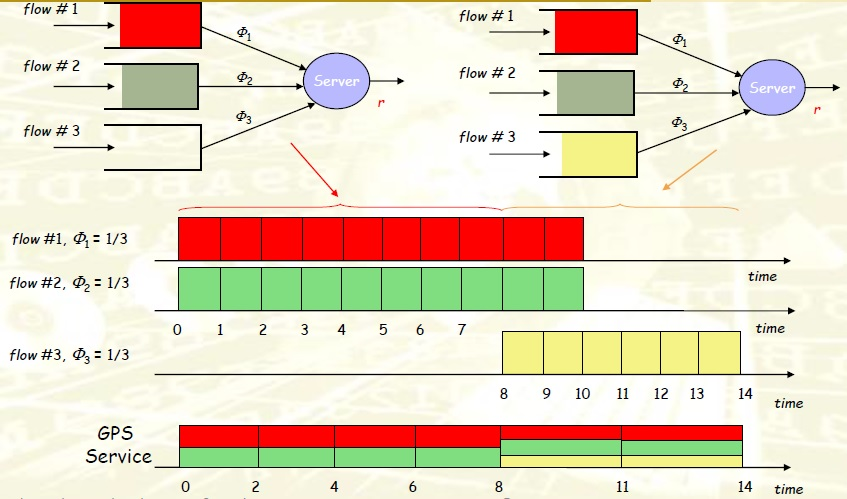
\includegraphics[scale=0.5]{figures/gps.jpg}
    \caption{GPS - funzionamento}
\end{figure}
In figura possiamo vedere il funzionamento di GPS. In particolare, ogni quadretto sulla linea temporale rappresenta un pacchetto. Da t=0 a t=7 abbiamo solo due flussi in arrivo al server, ciascuno occupando 1 unità di tempo per pacchetto. Da t=8 in poi, i flussi diventano tre (quindi 3 unità di tempo).\\
GPS è un algoritmo conservativo per cui la disuguaglianza:\\
\begin{center}
\( \displaystyle \frac{W\textsubscript{i}(t\textsubscript{1}, t\textsubscript{2})}{\phi\textsubscript{i}} \geq \frac{W\textsubscript{j}(t\textsubscript{1}, t\textsubscript{2})}{\phi\textsubscript{j}}\), j=1,2,...,N
\end{center}
è verificata per qualsiasi flusso i che è continuamente arretrato (backlogged) nell'intervallo \( [t\textsubscript{1}, t\textsubscript{2}] \). In altre parole, se la coda del buffer è sempre non-vuota, allora il servizio relativo (relativo alla mia frazione di banda) che ricevo non può essere minore del servizio normalizzato ricevuto da qualsiasi altro flusso, nello stesso intervallo.
Se entrambi i flussi i e j sono entrambi arretrati (backlogged) in \( [t\textsubscript{1}, t\textsubscript{2}] \) allora si ha un'uguaglianza. Rispetto all'Indice di Golestani (o Relative Fairness Index), GPS è perfettamente fail in quanto i due termini della sottrazione sono uguali e quindi RFI = 0.\\
Ad un flusso i viene garantito un certo \textit{rate minimo} g\textsubscript{i} calcolabile come:
\[ \frac{W\textsubscript{i}(t\textsubscript{1}, t\textsubscript{2})}{W\textsubscript{j}(t\textsubscript{1}, t\textsubscript{2})} \geq \frac{\phi\textsubscript{i}}{\phi\textsubscript{j}}\]

\[ W\textsubscript{i}(t\textsubscript{1}, t\textsubscript{2})\phi\textsubscript{j} \geq W\textsubscript{j}(t\textsubscript{1}, t\textsubscript{2})\phi\textsubscript{i}\]

\[ \sum_{j=1}^{N} W\textsubscript{i}(t\textsubscript{1}, t\textsubscript{2})\phi\textsubscript{j} \geq \sum_{j=1}^{N} W\textsubscript{j}(t\textsubscript{1}, t\textsubscript{2})\phi\textsubscript{i} \]

\[ W\textsubscript{i}(t\textsubscript{1}, t\textsubscript{2})\sum_{j=1}^{N} \phi\textsubscript{j} \geq 
\phi\textsubscript{i}\sum_{j=1}^{N} W\textsubscript{i}(t\textsubscript{1}, t\textsubscript{2}) \]
A questo punto ci interessa notare che il termine \( \sum_{j=1}^{N} W\textsubscript{i}(t\textsubscript{1}, t\textsubscript{2}) \) indica la somma dei servizi forniti a tutti i flussi nell'intervallo \( [t\textsubscript{1}, t\textsubscript{2}] \) ma noi sappiamo che c'è almeno un flusso (i) che è sempre arretrato (backlogged). Quindi durante questo intervallo, sapendo che GPS è conservativo, possiamo dire che il server utilizza tutto il rate disponibile.\\
Detto questo, possiamo scrivere che (ricordando che \( r \) è il rate):

\[ \sum_{j=1}^{N} W\textsubscript{i}(t\textsubscript{1}, t\textsubscript{2}) = r(t\textsubscript{2}, t\textsubscript{1}) \]
Sostituendo nella disuguaglianza iniziale:
\[ W\textsubscript{i}(t\textsubscript{1}, t\textsubscript{2})\sum_{j=1}^{N} \phi\textsubscript{j} \geq
\phi\textsubscript{i} r(t\textsubscript{2} - t\textsubscript{1}) \]
e quindi:
\[ W\textsubscript{i}(t\textsubscript{1}, t\textsubscript{2}) \geq \frac{\phi\textsubscript{i}}{\sum_{j=1}^{N} \phi\textsubscript{j}}r(t\textsubscript{2} - t\textsubscript{1})\]
dove \( g\textsubscript{i} = \frac{\phi\textsubscript{i}}{\sum_{j=1}^{N} \phi\textsubscript{j}}r \)\\
La banda allocata in eccesso a dei flussi può essere redistribuita tra i flussi arretrati (backlogged) in proporzione al loro peso. In questo caso si parla di rate istantaneo. In figura possiamo osservare come varia il servizio ricevuto dal flusso i: la curva è limitata superiormente dalla capacità del link \( r\) ed inferiormente dal rate minimo garantito \( g\textsubscript{i} \). La pendenza non può mai essere in contrasto con le pendenze di queste due rette.
\begin{figure}[H]
    \centering
    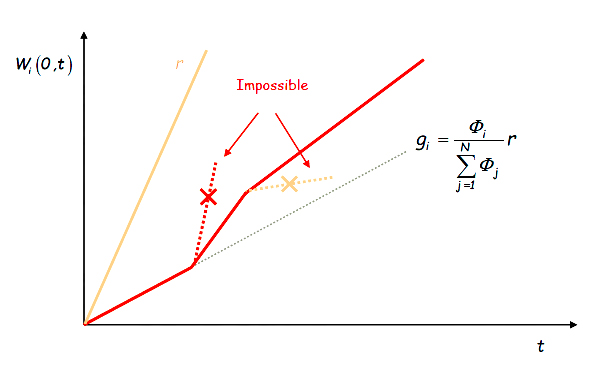
\includegraphics[scale=0.5]{figures/gps_rate.jpg}
    \caption{GPS - funzionamento}
\end{figure}
In conclusione, GPS non è realizzabile per davvero poiché introduce delle assunzioni che non sono realistiche:  i pacchetti non sono infinitamente divisibili e non possono essere trasmessi simultaneamente. Ma se implementassimo un algoritmo di scheduling che crea gli stessi output con lo stesso ordine (ma con tempistiche diverse)?

\subsubsection{WFQ - Weighted Fair Queueing}
Algoritmo conservativo che simula il comportamento di GPS mandando i pacchetti in uscita nello stesso ordine, ma con tempistiche diverse. Anche questo algoritmo non è realizzabile praticamente.\\
Trasmette pacchetti scegliendo, tra quelli in coda all'istante t, quello che completerebbe il servizio per primo se il sistema fosse GPS e nessun altro pacchetto arrivasse dopo l'istante t. In altre parole, sappiamo che in GPS i pacchetti possono essere serviti contemporaneamente mentre in WFQ no. Quindi l'algoritmo servirà i pacchetti singolarmente ma nello stesso ordine di GPS. Questo significa che l'output sarà il solito (nello stesso ordine) ma il tempo a cui usciranno i vari pacchetti sarà diverso.
\paragraph{Esempio} Supponiamo che un pacchetto \(p\) sia in servizio presso un sistema GPS ed uno WFQ. Ad un istante generico \(t\) arriva un nuovo pacchetto \(p'\). Nel caso di GPS il pacchetto inizia subito il servizio (simultaneamente a \(p\) ed uscirà all'istante \(t+n\). Con WFQ il pacchetto inizierà il servizio non appena terminerà quello di \(p\) ed uscirà ad un istante \(t+m\) con \( m>n\). L'ordine di uscita sarà sempre \(p, p'\) ma il tempo a cui escono i due pacchetti sarà diverso.\\ \\
Si può dire quindi che WFQ approssima il comportamento di GPS, ma fino a che punto? La differenza tra i due algoritmi è data dalla differenza dei tempi d'uscita per un singolo pacchetto, ed è limitata dalla MTU (Maximum Transfer Unit):
\[ out\textsubscript{WFQ} - out\textsubscript{GPS} \leq MTU \]
Possiamo avere 2 casi: o siamo in ritardo rispetto a GPS, e quindi possiamo esserlo al più del tempo necessario a trasmettere un pacchetto di dimensione = MTU, oppure siamo in anticipo rispetto a GPS (ma questo non è possibile per questioni di fairness). Vediamo un esempio di come WFQ non sia \textit{fair}.
%fairness1
\begin{figure}[H]
    \centering
    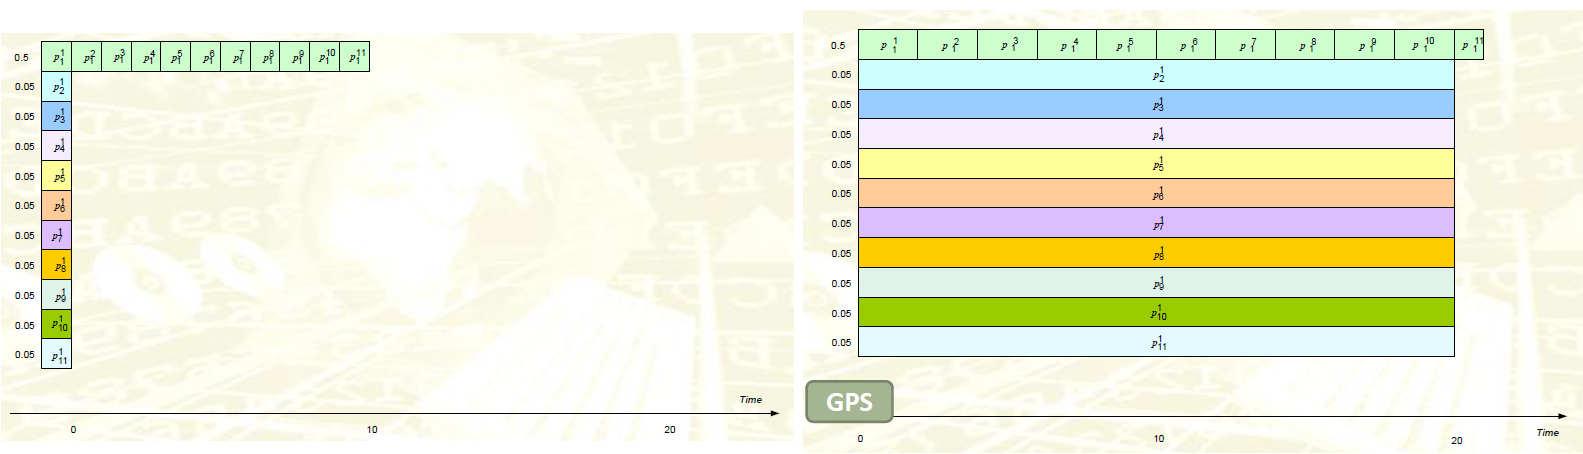
\includegraphics[scale=1.1]{figures/fairness1.jpg}
    \caption{}
\end{figure}
In figura possiamo osservare l'ordine di arrivo dei pacchetti (sx) e l'ordine di servizio in un sistema GPS (dx). Il servizio in uscita offerto dal sistema WFQ sarà:
%fairnsess2
\begin{figure}[H]
    \centering
    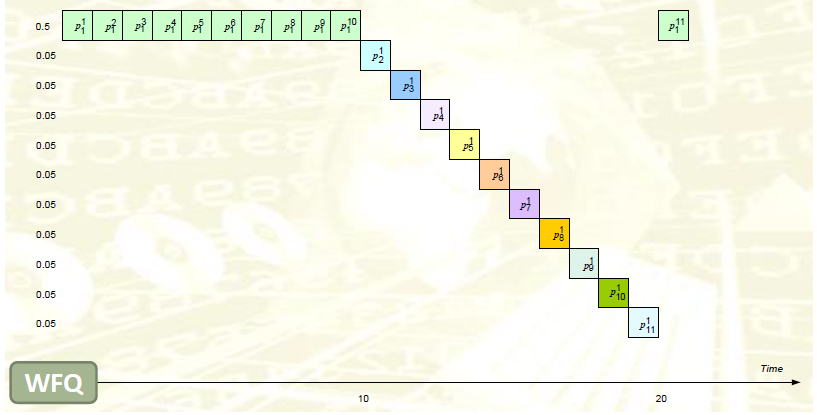
\includegraphics[scale=1.7]{figures/fairness2.jpg}
    \caption{Servizio del sistema WFQ}
\end{figure}

%\paragraph{Busy Period} E' un intervallo di tempo in cui il server è occupato. Per un server di tipo conservativo, l'inizio e la fine del busy period non dipendono dalla disciplina di scheduling.

\newpage
\subsubsection{(WF)\textsuperscript{2}Q - Variante di WFQ}
Worst-case Fair WFQ è una variante di WFQ che, quando il server è pronto a trasmettere un nuovo pacchetto ne sceglie uno fra quelli che avrebbero già cominciato ad essere serviti da un sistema GPS equivalente. Tornando all'esempio fatto nel capitolo precedente, vediamo come cambia il servizio del sistema WFQ:
%fairnsess3
\begin{figure}[H]
    \centering
    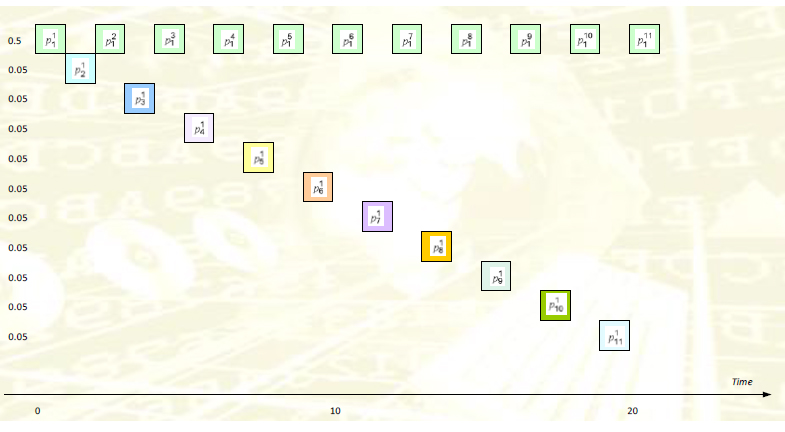
\includegraphics[scale=2]{figures/fairness3.jpg}
    \caption{Servizio del sistema WF\textsuperscript{2}Q}
\end{figure}
Come si può osservare, il primo pacchetto ad uscire è sempre p\textsubscript{1}\textsuperscript{1} in quanto è il primo ad arrivare. Tuttavia, quando p\textsubscript{1}\textsuperscript{1} viene trasmesso il prossimo ad essere preso in lavorazione non sarà p\textsubscript{1}\textsuperscript{2} in quanto non ancora arrivato, bensì p\textsubscript{2}\textsuperscript{1}. In questo modo i pacchetti del flusso 1 si alternano con tutti gli altri.

\newpage
\subsubsection{DRR - Deficit Round Robin}
Algoritmo di packet-scheduling conservativo, basato su frame (temporali). I flussi sono organizzati in una lista circolare e vengono controllati (in ordine) uno alla volta per vedere se hanno pacchetti da trasmettere. Ogni flusso può trasmettere un numero massimo di pacchetti per ogni round.\\
Ciascun flusso i è caratterizzato da:
\begin{itemize}
    \item un quanto Q\textsubscript{i} di unità di traffico (bit, byte ecc.) che misura la quantità di traffico che il flusso i dovrebbe \textit{idealmente} trasmettere. Perché idealmente? Perché un flusso potrebbe avere meno unità di traffico da trasmettere al momento in cui viene interrogato, oppure la dimensione del pacchetto potrebbe non coincidere perfettamente con Q\textsubscript{i} (cioè il quanto non è multiplo della dimensione del pacchetto).
    \item un Deficit Counter (DC\textsubscript{i}): serve a tener traccia dei byte totali inviati da un flusso, in questo modo si possono recuperare eventuali byte non sfruttati nel round precedente (a causa del fatto che il quanto non era multiplo della dimensione del pacchetto).
\end{itemize}
Funzionamento:
\begin{enumerate}
    \item Quando un flusso è \textit{backlogged}, DC\textsubscript{i} = 0
    \item Ad ogni round, DC\textsubscript{i} = DC\textsubscript{i} + Q\textsubscript{i}
    \item Il flusso \(i\) può trasmettere fino a DC\textsubscript{i} pacchetti
    \item Se il flusso è ancora \textit{backlogged} dopo il servizio, DC\textsubscript{i} = DC\textsubscript{i}- byte(trasmessi)
    \item Altrimenti, se \(i\) non è più \textit{backlogged}, DC\textsubscript{i} = 0
\end{enumerate}
Notare che DC\textsubscript{i} è limitato superiormente dalla dimensione massima di un pacchetto. Se un flusso deve trasmettere un pacchetto con \( dim(pkt) > Q\textsubscript{i} \) allora accumulo tutto Q\textsubscript{i} nel deficit. Se al prossimo round \( dim(pkt) > Q\textsubscript{i} \), accumulo di nuovo e così via fino a che, eventualmente, \( DC\textsubscript{i} = dim(pkt) \) e quindi potrò trasmettere.\\
\newpage
\section{DiffServ}
Soluzione che fornisce la possibilità ai router di differenziare i flussi in classi in modo tale che, all'interno del dominio DiffServ, ogni pacchetto appartenente alla stessa classe venga trattato allo stesso modo. C'è un numero fisso di classi QoS. La classificazione del traffico viene fatta al \textbf{confine} del dominio DiffServ, ossia all'interfaccia d'ingresso di un "border router".\\
Non si potrebbe delegare questo compito all'applicazione? In teoria si, ma non vogliamo che questo accada perché significherebbe standardizzare le classi QoS in tutta la rete internet.\\

\subsection{Traffic Classification}
Processo di identificazione dei pacchetti e di assegnamento di una classe, con lo scopo di applicare un'azione comune ad essi. Esistono diversi metodi per classificare i pacchetti:
\begin{itemize}
    \item Complesso: detta anche multi-campo, si basa sul valore di campi specifici all'interno dell'header IP (per esemio sorgente/destinazione o porta UDP o TCP).
    \item DPI (Deep Packet Inspection): controlla anche i dati del pacchetto.
    \item Semplice: riguarda campi dell'header progettati appositamente per la classificazione QoS.
\end{itemize}
\subsection{Traffic Conditioning} Meccanismo tramite il quale possiamo:
\begin{itemize}
    \item Policing: Imporre regole al  flusso di traffico per far rispettare un determinato profilo di burst/rate. Solitamente i pacchetti non conformi sono scartati.
    \item Shaping: Riformare (ritardare pacchetti) in un flusso di traffico per far rispettare quanto sopra. I pacchetti non conformi vengono modificati in modo da esserlo.
\end{itemize}
Concretamente questo significa che nel router andremo a definire i vari gruppi (classi) e come classificare i flussi di traffico nei gruppi. Dopodiché, per ogni gruppo, stabiliamo un "profilo" che ogni flusso appartenente a quel gruppo deve rispettare per essere ammesso nel dominio DiffServ.\\

\subsubsection{Policing}
Un metodo per implementare il policing è il \textit{token bucket}, ossia un contenitore dentro al quale disporremo dei "gettoni" virtuali. Inizialmente il bucket è pieno. Un pacchetto, per poter trasmettere, ha bisogno di un numero di token pari alla sua dimensione.\\

% Define block styles
\tikzstyle{decision} = [diamond, draw, 
    text width=4.5em, text badly centered, node distance=3cm, inner sep=0pt]
\tikzstyle{block} = [rectangle, draw, 
    text width=7em, text badly centered, rounded corners, minimum height=4em]
\tikzstyle{line} = [draw, -latex']
    
\begin{tikzpicture}[node distance = 3cm, auto]
    % Place nodes
    \node [block] (init) {Arriva pacchetto dimensione \textit{n}};
    \node [decision, right of=init, node distance=4cm] (identify) {\textit{n} token nel bucket?};
    \node [block, fill=red!20, below of=identify, node distance=3cm] (exceed) {exceed action};
    \node [block, right of=identify, node distance=4cm] (update) {decremento token count di \textit{n}};
    \node [block, right of=update, fill=green!20, node distance=4cm] (stop) {conform action};
    % Draw edges
    \path [line] (init) -- (identify);
    \path [line] (identify) -- node {no} (exceed);
    \path [line] (identify) -- node {si} (update);
    \path [line] (update) -- (stop);
\end{tikzpicture}
A questo punto bisognerà definire in cosa consistono le azioni di \textit{exceed} e \textit{conform} in base al comportamento che vogliamo ottenere.

\subsubsection{Shaping}
In questo caso, se non ci sono abbastanza token nel bucket il pacchetto non viene scartato, bensì viene messo in attesa fino a che non ci saranno token a sufficienza.\\

\begin{tikzpicture}[node distance = 3cm, auto]
    % Place nodes
    \node [block] (init) {Arriva pacchetto dimensione \textit{n}};
    \node [decision, right of=init, node distance=4cm] (identify) {\textit{n} token nel bucket?};
    \node [block, below of=identify, node distance=3cm] (exceed) {Attendo che ci siano i token};
    \node [block, right of=identify, node distance=4cm] (update) {decremento token count di \textit{n}};
    \node [block, right of=update, fill=green!20, node distance=4cm] (stop) {Trasmetti};
    % Draw edges
    \path [line] (init) -- (identify);
    \path [line] (identify) -- node {no} (exceed);
    \path [line] (identify) -- node {si} (update);
    \path [line] (update) -- (stop);
    \path [line] (exceed) -| (update);
\end{tikzpicture}

\subsection{DiffServ Code Point}
Nuovo campo da 6bit introdotto nei pacchetti IP per permettere la classificazione dei pacchetti in classi corrispondenti ad un PHB (Per-Hop Behaviour). Questi 6 bit possono essere usati liberamente all'interno di un dominio DiffServ purché pacchetti appartenenti allo stesso flusso abbiano la stessa classe PHB. Di default, i pacchetti hanno la classe \textbf{CS0} detta anche best-effort.\\

\begin{figure}[H]
    \centering
    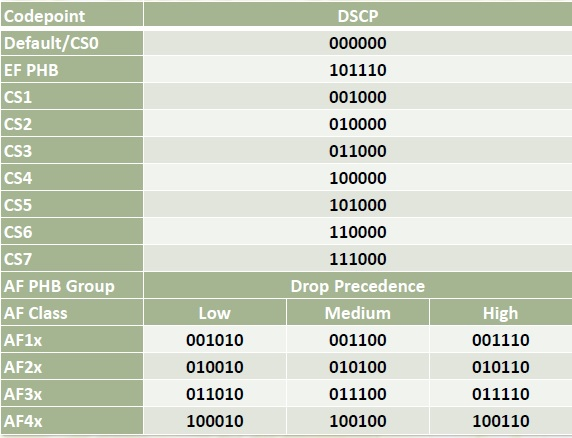
\includegraphics[scale=0.5]{figures/dscp.jpg}
    \caption{Codici DSCP}
\end{figure}

\paragraph{Expedited Forwarding (EF)} Se un pacchetto è marcato con questa classe EF, allora a quel pacchetto è garantito un rate minimo indipendente dal carico del traffico non-EF. Questa classe è particolarmente utile per applicazioni che necessitano basso ritardo e poca perdita di pacchetti (esempio: VoIP).
\paragraph{Assured Forwarding (AFxy)} Set di classi pensate per un tipo di traffico che non ha particolari requisiti in termini di latenza. Per questo, il traffico out-of-profile verrà lasciato passare ugualmente (a meno che non crei congestione nella rete, in quel caso verrà rimosso). Abbiamo 12 possibili gruppi per AF: i primi 3 bit x identificano la classe (1-4) mentre i successivi 2 bit y servono a stabilire la precedenza di drop all'interno della stessa classe (low, med, high).\\

\subsection{Active Queue Management}
In che modo vengono scartati i pacchetti? Tradizionalmente ciò avviene quando un pacchetto arriva all'ingresso della coda ma non c'è abbastanza spazio per contenerlo. Questa strategia è chiamata \textbf{tail drop}. Il motivo per cui si scartano i pacchetti non è perché non c'è abbastanza memoria per gestire le code ma perché code più lunghe implicano ritardi maggiori dovuti al tempo di accodamento.\\
Per fornire un trattamento diverso alle classi di pacchetti, potremmo usare una tecnica nota come \textbf{tail-drop pesato}. Supponiamo che la coda abbia due limiti \(q\textsubscript{1}\) e \(q\textsubscript{2}\) con \(q\textsubscript{1} < q\textsubscript{2} \). Quando un pacchetto a bassa priorità arriva, viene scartato se la dimensione della coda è maggiore di \(q\textsubscript{1}\). Quando arriva un pacchetto ad alta priorità, si applica invece la soglia \(q\textsubscript{2}\).\\
Quando avviene il drop del pacchetto, il mittente (tipicamente) reagisce diminuendo il suo rate di trasmissione che, teoricamente, porterebbe ad un'ottimizzazione del throughput dell'applicazione. Questo in realtà non è sempre vero poiché se tutti i mittenti spediscono pacchetti simultaneamente, questi vengono scartati. A questo punto i mittenti reagiscono diminuendo il rate di trasmissione e si arriva ad uno scenario in cui si è passati ad una bassa utilizzazione della rete. Questo problema è noto come \textit{global synchronization}.\\
Per questi motivi viene sviluppato l'Active Queue Management, un insieme di tecniche volte a gestire le code di un router in modo da limitare il ritardo e ottimizzare il throughput.\\

\subsubsection{RED - Random Early Detection}
Tecnica pro-attiva pensata per rilevare preventivamente una possibile congestione e per fornire feedback alle applicazioni. La congestione è rilevata tramite l'osservazione della lunghezza (profondità) media della coda. Raggiunta una certa soglia di riempimento, se arriva un nuovo pacchetto, viene deciso in maniera casuale se scartarlo o meno. In questo modo solo uno (o pochi più) dei flussi diminuirà (diminuiranno) il rate. Abbiamo quindi evitato il problema della \textit{global synchronization}.

\begin{figure}[H]
    \centering
    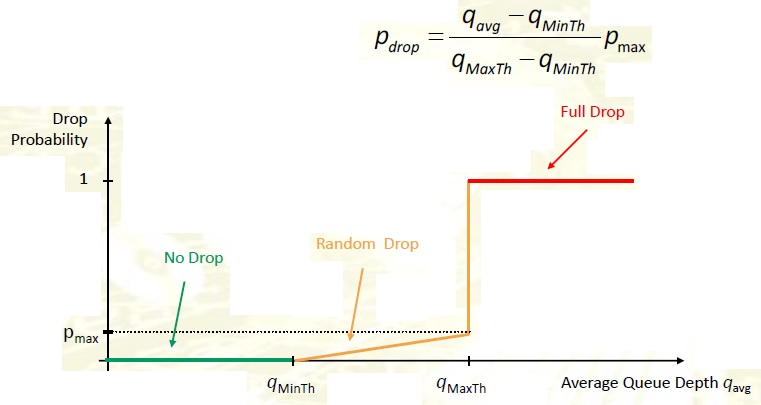
\includegraphics[scale=0.5]{figures/red.jpg}
    \caption{Random Drop}
\end{figure}
Come possiamo vedere in figura, ad ogni soglia \(q\) della coda corrisponderà una certa probabilità di drop. Possiamo rendere l'algoritmo più o meno \textit{aggressivo} andando a modificare la pendenza della retta di random drop. Questo può essere utile nel caso delle classi DSCP perchè ci permette di avere un comportamento di RED diverso per ogni classe, a seconda della loro precedenza di drop.

\newpage
\section{Core Network Protocols and Architectures}
\subsection{MPLS - Problema}
Con l'espansione della rete, sono nati problemi di scalabilità di gestione delle reti. Ogni router contiene tabelle di routing/forwarding per l'inoltro dei pacchetti, generate dagli algoritmi. Per inoltrare un pacchetto a destinazione, dovrà essere presente un'entrata nella tabella di routing per la destinazione. \\ Il dominio della rete è composto da border router e core. Questo dominio deve consegnare i pacchetti a diverse destinazioni, l'inoltro avviene ad ogni hop. Se un pacchetto arriva ad un certo border router e deve uscire da un altro border router, dovrà seguire un determinato percorso nel dominio. L'inoltre del pacchetto è basato sull'indirizzo destinazione contenuto nel pacchetto. Ad ogni router viene scelto il next hop in base alla tabella di routing, che è conosciuta solo al router che la possiede e che mappa DEST, ADD e NEXT HOP. Quando un pacchetto arriva ad un router è necessario che vi sia corrispondenza, cioè l'indirizzo di destinazione indicato nel pacchetto deve essere presente nella tabella. Più si è interni al core della rete, più la tabella di routing sarà grande. \\ Quindi, più sono i nodi più saranno le entrate necessarie nella tabella di routing. Si crea quindi un problema di scalabilità. Quando un router interno deve mandare un pacchetto all'esterno, seleziona il miglior border router tra quelli disponibili e gli inoltra il pacchetto. Nella tabella di routing ci saranno le entrate per i nodi del dominio e per le network esterne che si annunciano al BR. \\ Il problema principale, quindi, risiede nel fatto che per ogni "nuova" rete esterna che si annuncia, si deve aggiornare la tabella di routing di ogni router all'interno al dominio. Questo approccio, come si può immaginare, non scala bene in quanto si ha un aumento della dimensione della tabella di routing senza che nel dominio siano aggiunti nuovi nodi. \\ Si avrà quindi bisogno di uno strumento nei core router che ci dica, per ogni destinazione esterna, quale sia il BR a cui inoltrare il pacchetto. In questo modo solo i BR aggiorneranno la loro tabella con gli annunci esterni al dominio. Non c'è alcun modo di fare questo con IP.
\begin{figure}[H]
    \centering
    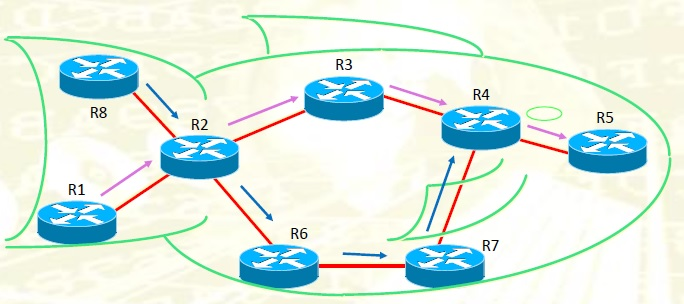
\includegraphics[scale=0.6]{figures/fish.jpg}
    \caption{Esempio di \textit{fish-network}}
\end{figure}
Un esempio lampante per capire il problema è quello della "fish network" mostrato in figura, in cui si hanno 2 flussi distinti che devono raggiungere un certo border router. Assumendo che uno dei percorsi per raggiungere il border router sia più lento e l'altro più veloce, vorremmo decidere di differenziare i 2 flussi nei due percorsi differenti. Questo con IP non è possibile, perché il path in IP viene deciso solo tramite il destination address. Tutti i flussi di dati vengono trattati ugualmente, non è possibile modificare questo comportamento del protocollo IP. Quindi, l'obiettivo è che un percorso non venga scelto solo attraverso la destinazione, ma anche sulla base della sorgente. \\ Per risolvere il problema, si deve fare \textit{reverse-engineering} su OSPF, modificando il costo del link, in modo tale che il risultato dato in output da OSPF sia uguale a quello che abbiamo calcolato esternamente. Tramite questo lavoro si ottimizzano le performance della rete. \\ MPLS (Multi-Protocol Label Switching) si pone come soluzione per risolvere problemi di questo tipo.

\newpage
\subsection{MPLS - Funzionamento}
\subsubsection{Concetto Label Switching}
Si va a modellare il processo di forwarding all'interno dei router. Può essere diviso in 2 fasi:
\begin{itemize}
    \item \textbf{Partizionamento: } I pacchetti vengono divisi in classi dette FEC (Forwarding Equivalent Class). La FEC di un pacchetto nel classico forwarding IP viene scelta guardando solamente il Destination Address (che è quello che vogliamo cambiare con MPLS). Pacchetti che appartengono alla stessa FEC vengono trattati allo stesso modo dal router.
    \item \textbf{Mappatura: }  Ogni FEC è mappata dal router verso un determinato next hop creando così una corrispondenza ben precisa.
\end{itemize}
In tutto questo assumiamo che tutti i router del dominio abbiano la stessa visione su come partizionare i pacchetti in FEC, ovvero siano d'accordo su quali siano le classi FEC.\\
Il partizionamento e la mappatura, nel forwarding IP convenzionale, vengono effettuati ad ogni hop. Nel nostro approccio si vanno a dividere, il partizionamento viene effettuato negli edge router (router di ingresso) mentre la mappatura viene fatta ad ogni hop. \\ Questo perché, la fase di partitioning è molto complessa, dato che potenzialmente coinvolge l'ispezione di molti campi di un pacchetto. Come conseguenza di questa suddivisione di ruoli, si deve assegnare un label ai pacchetti in modo che i core router possano identificare a quale FEC appartengono i pacchetti. Un valore della label L corrisponde ad una specifica classe e viene inserito all'interno del pacchetto. \\ Questo approccio cambia la struttura delle tabelle di forwarding, che adesso hanno un mapping tra il label e il next hop. È molto conveniente, dato che consente di ripetere il partitioning ad ogni router che, come detto precedentemente, è ritenuta un'operazione molto dispendiosa. Il label è un campo "piccolo" e quindi di facile ispezione, rispetto ad eventuali altri campi (ad esempio il destination address). \\ Questa soluzione, inoltre, migliora il problema della scalabilità: quando diventa raggiungibile un nuovo network esterno, abbiamo bisogno di aggiornare soltanto i router di ingresso, in modo tale che pacchetti indirizzati alla "nuova" destinazione, siano mappati con una FEC associata al cammino che porta all'appropriato router di uscita. Mentre, i router interni non hanno bisogno di nessun update, perché sono già in grado di mappare quella FEC al prossimo hop, ovvero esiste già un cammino associato a quella specifica FEC. \\ Per implementare questa funzionalità descritta, abbiamo bisogno di un modo per consentire ai router di accordarsi a quale label associare a ogni FEC. Questo task potrebbe risultare abbastanza difficile, infatti si è trovato un modo per "aggirare" questo problema: si consente ad ogni router di scegliersi i label per rappresentare i FEC. I router si scambiano le informazioni con i propri vicini riguardo la rappresentazione usata, cosicché quando uno di questi deve trasmettere un pacchetto ad un vicino, semplicemente cambia il label associato al pacchetto giusto prima di effettuare la trasmissione, in modo da conformarsi con la rappresentazione utilizzata dal vicino.

\subsubsection{Architettura MPLS}
\paragraph{Piano dati MPLS} La figura \ref{figura:dati-mpls} rappresenta un esempio pratico di come viene gestito MPLS dai vari router, sul piano dati. Nell'immagine, i nodi ai bordi vengono chiamati "edge" e quelli interni "core". \\ I router coinvolti in questa operazione vengono definiti con il termine \textit{Label Switching Routers (LSR)}. 
\begin{figure}[H]
    \centering
    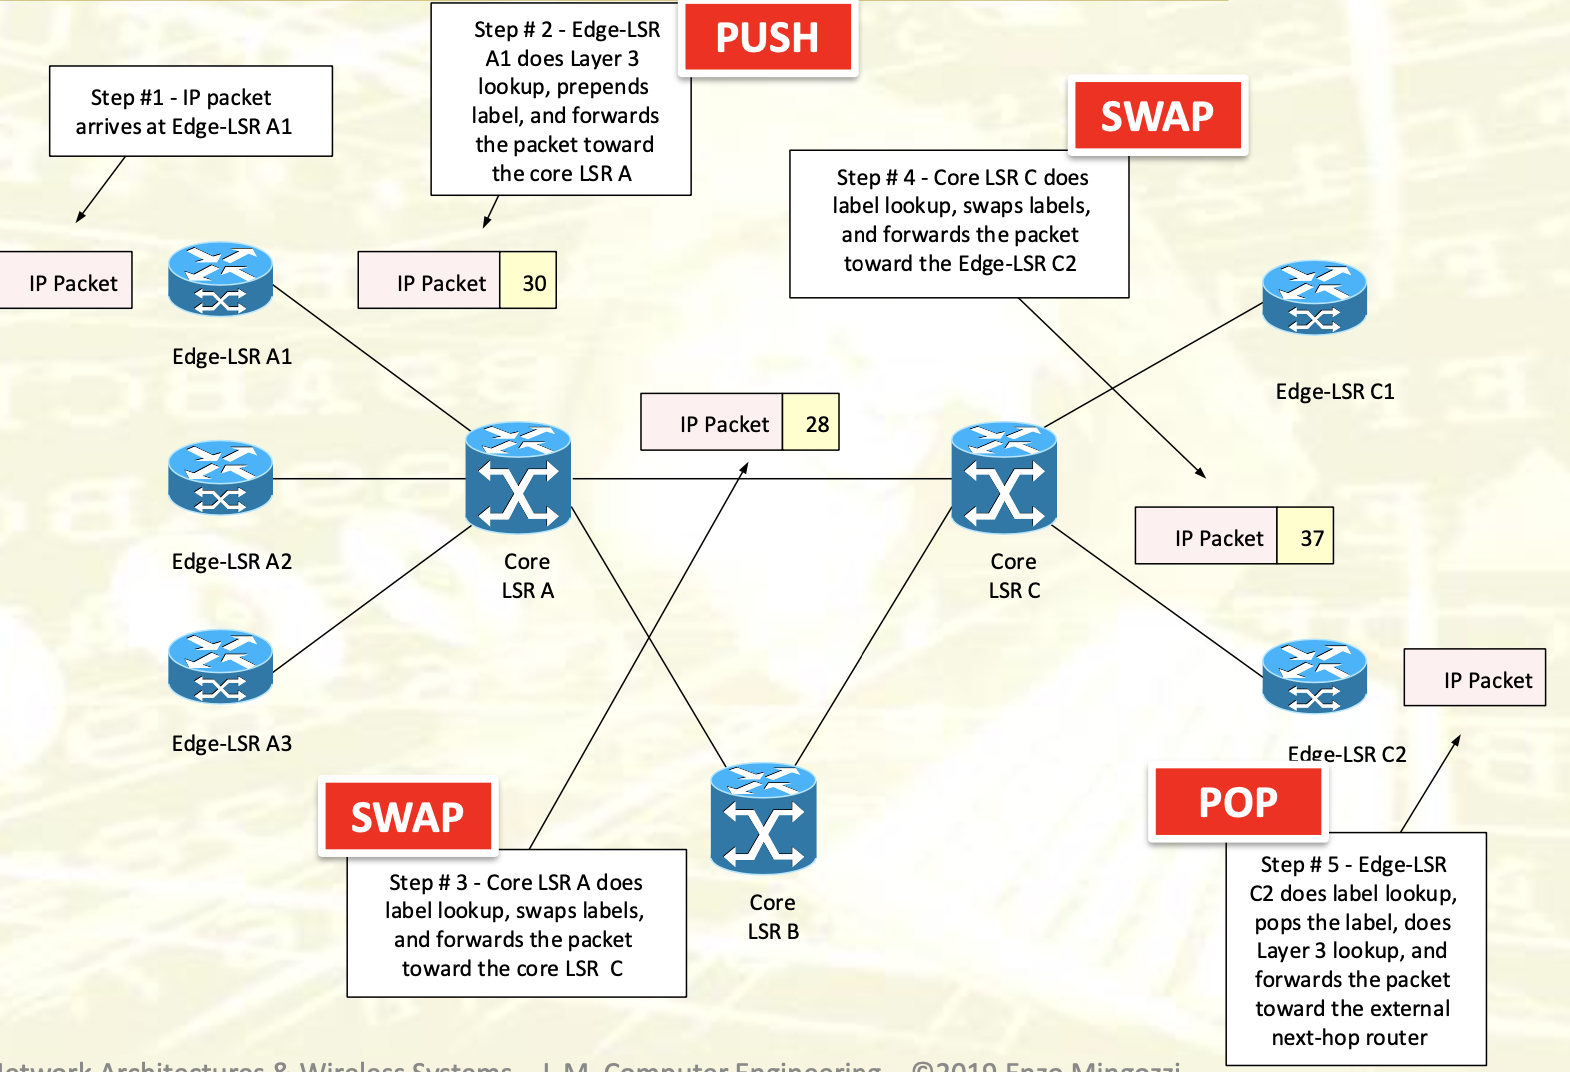
\includegraphics[scale=0.4]{figures/mpls data plane.png}
    \caption{MPLS data plane}\label{figura:dati-mpls}
\end{figure}
Supponendo che arrivi un pacchetto al router A1. Questo è inizialmente privo di etichetta; deve quindi essere specificata la classe di inoltro del pacchetto, quindi al successivo nodo viene mandato il pacchetto IP ed in più la nuova informazione riguardante la classe. Questa operazione di etichettamento viene chiamata \textit{PUSH} (il cui nome viene preso dalle tipiche operazioni effettuate su uno stack). Quando il pacchetto arriva al Core LSR A, questo riceve un pacchetto che già possiede un'etichetta, quindi lo inoltrerà, a seconda dell'etichetta, al prossimo hop. Prima di inoltrare un pacchetto, però, viene sostituito il valore dell'etichetta del pacchetto ricevuto con un valore utile a permettere al prossimo nodo di identificare la classe del pacchetto: operazione di \textit{SWAP}. Stessa cosa per il Core LSR C, e così via fino a giungere al router finale: se il pacchetto deve uscire dal dominio, l'ultimo router farà un operazione di \textit{POP}, ovvero rimuove l'etichetta al pacchetto, facendolo tornare come era prima di entrare nel dominio.
\subparagraph{Codifica del label} Il label viene codificato in una stringa di bit lunga almeno 32 bit. Se sono presenti più etichette, ci saranno altrettanti blocchi da 32 bit, posizionati in una sorta di stack (da qua, i nomi relativi alle operazioni menzionati nel paragrafo precedente).
\begin{figure}[H]
    \centering
    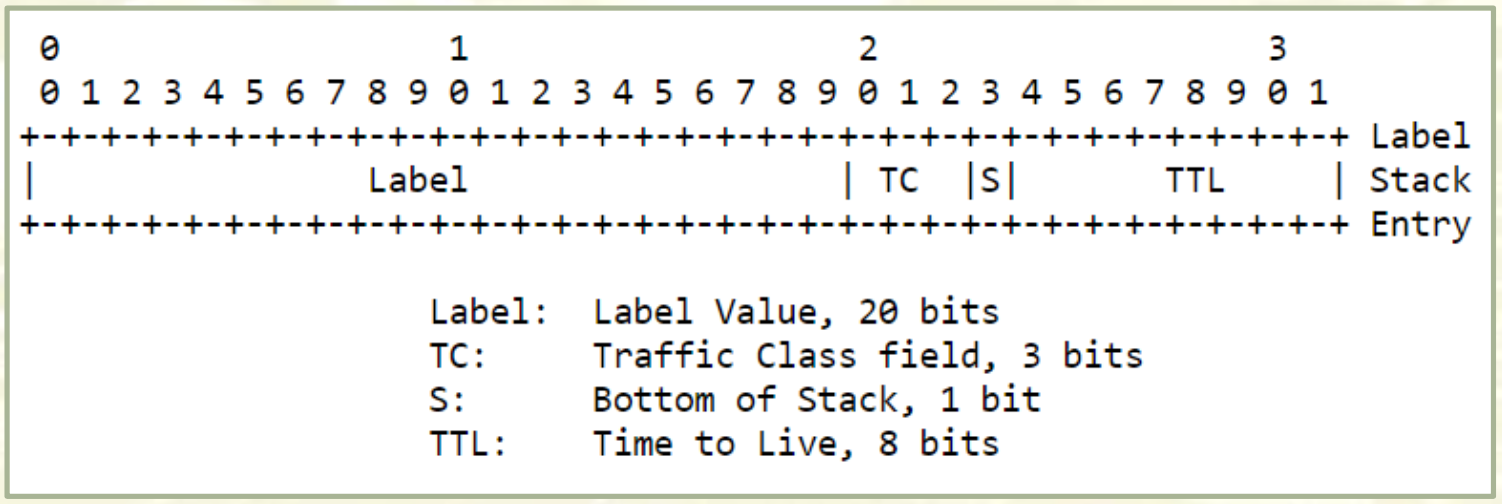
\includegraphics[scale=0.4]{figures/mpls header.png}
    \caption{Formato dell'header}
\end{figure}
Nello specifico, i campi vengono definiti nel seguente modo:
\begin{itemize}
    \item \textbf{Label:} è un identificatore corto, di lunghezza fissata e significativo solo localmente. Viene utilizzato per identificare un FEC.
    \item \textbf{Traffic Class (TC):} identifica la classe di traffico di appartenenza del pacchetto, per introdurre una differenziazione di trattamento dei pacchetti con uguale etichetta.
    \item \textbf{Time-to-Live (TTL):} nello stile di IPv4 o IPv6. Serve a garantire che in percorsi ciclici il pacchetto non giri all'infinito.
    \item \textbf{S:} Flag che serve a gestire la pila. Nello specifico, il flag è settato se l'header si riferisce all'etichetta che si trova in fondo alla pila. Quando ci sono più header, si riconoscerà l'ultimo in fondo alla pila grazie a questo flag. Se non ci sono flag a 1, significa che il prossimo header è il pacchetto IP stesso.
\end{itemize}
Per ogni protocollo di livello 2, c'è un modo per il ricevitore di sapere che i successivi 4 byte sono MPLS e non occorre leggere altro oltre questi 4 byte per sapere come effettuare il forwarding. Si parla di layer 2.5, perché l'header si pone, appunto, in mezzo ai layer 2 e 3. Quindi, per ogni tecnologia di livello 2, bisogna specificare un valore per il tipo di payload che identifichi che il prossimo layer è MPLS. \\ Questo, però, non succede nel layer di MPLS, cioè non esiste un campo che identifichi quale protocollo sia il successivo, l'informazione viene considerata implicita. Ad esempio, si suppone che tutti i router usino IP. In alternativa si possono utilizzare classi diverse per specificare differenti tipi di payload.
\subparagraph{Modello funzionale MPLS}
Composto da 3 strutture dati:
\begin{itemize}
    \item \textbf{Next Hop Label Forwarding Entry (NHLFE):} che contiene le informazioni che riguardano l'azione da eseguire sul pacchetto (push, pop, swap), i parametri relativi a quella azione (se faccio un'azione devo conoscere il valore da inserire) e il next hop.
    \item \textbf{Incoming Label Map:} viene usata quando abbiamo un pacchetto in arrivo con un'etichetta già applicata. In questa mappa ci sono dei puntatori alla NHLFE e a seconda della label nell'etichetta del pacchetto vado a fare una delle azioni della NHLFE.
    \item \textbf{FEC-to-NHLFE Map:} fa un mapping tra FCE e label. A seconda della classe scelta, andiamo a fare un push dell'etichetta con il corrispondente valore del label.
\end{itemize}
Se il next hop è il router \textit{LSRx}, si fa una POP, ovvero si toglie l'etichetta. Il pacchetto ritorna allo stesso router (LSRx infatti indica lo stesso router che sta processando il pacchetto al momento), che, se non ci saranno più etichette, lo inoltrerà al Next Hop come un normale pacchetto IP.
\begin{figure}[H]
    \centering
    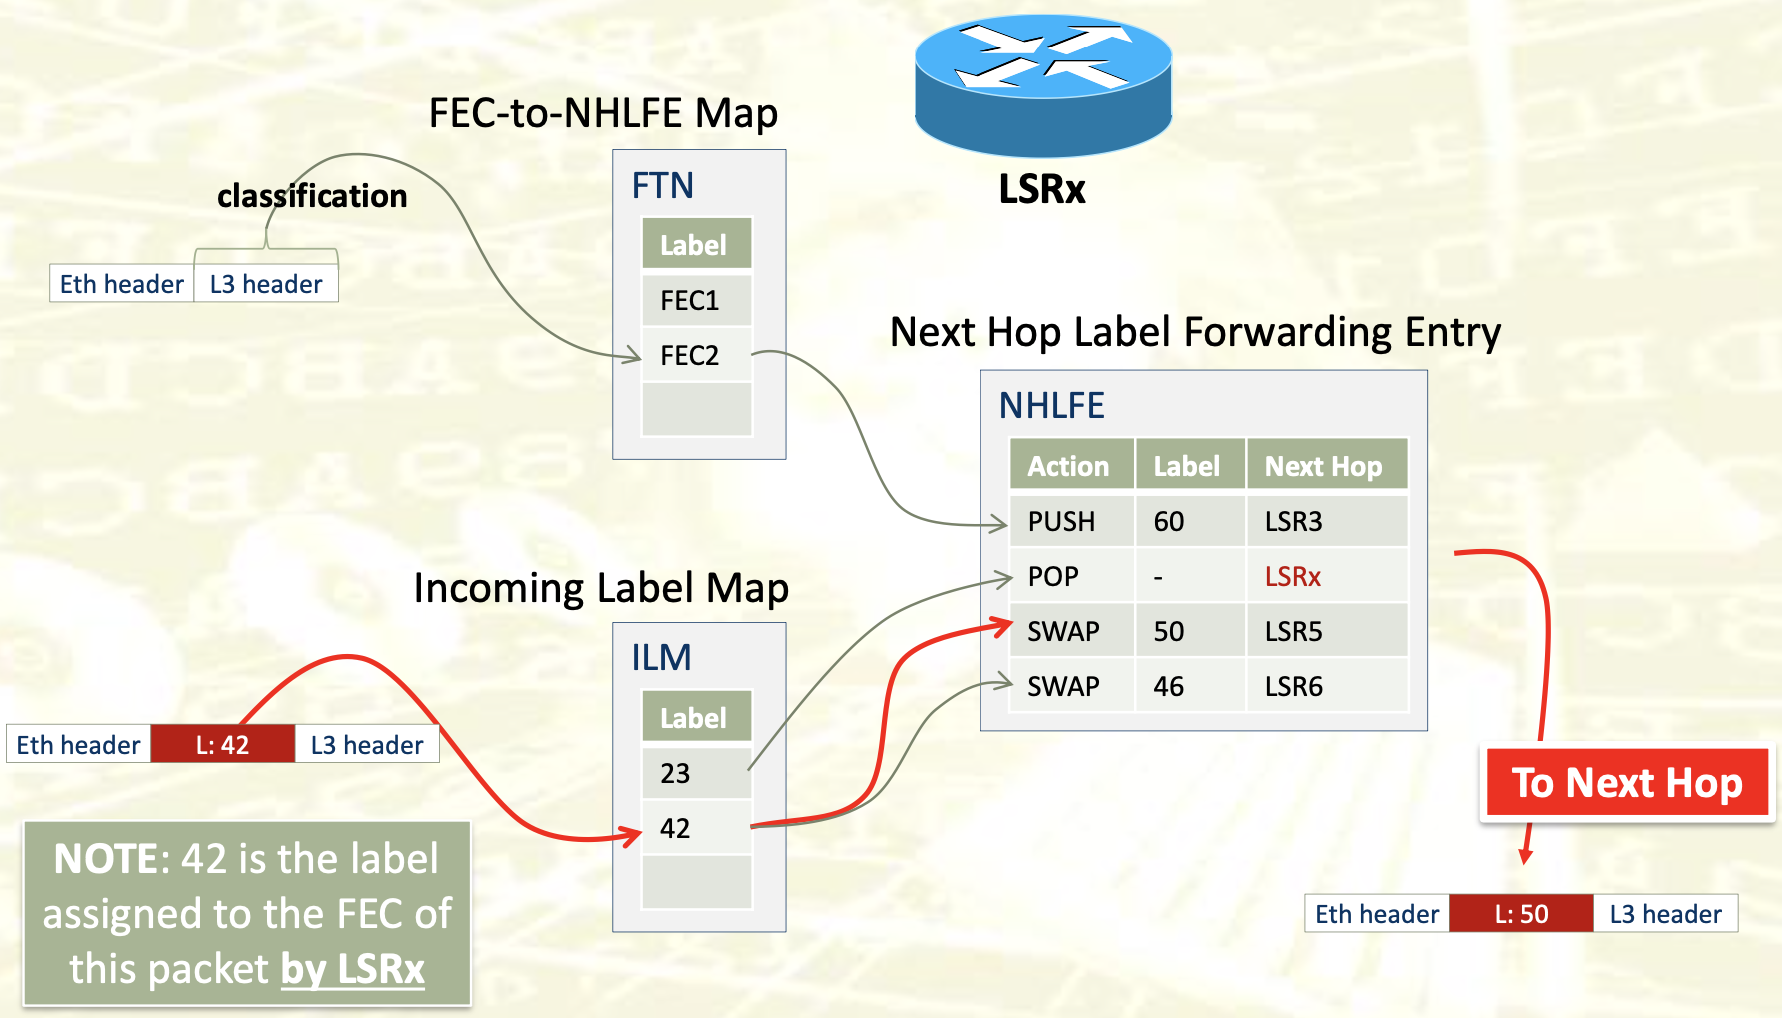
\includegraphics[scale=0.3]{figures/mpls strutture dati.png}
    \caption{Strutture dati di MPLS}
\end{figure}
Quello presentato è uno schema generale, le implementazioni reali potrebbero utilizzare strutture dati organizzate in modi differenti o con nomi diversi. In generale, si identificano con il nome generico di \textit{Label Forwarding Information Base}.
\subparagraph{Label Switched Path (LSP)} Un LSP è un path unidirezionale, identifica l'insieme delle informazioni correlate distribuite nelle varie Label Forwarding Information Base e che definiscono il percorso da ingresso a uscita. LSP non introduce meccanismi legati alla connessione e non è un tunnel.
\begin{figure}[H]
    \centering
    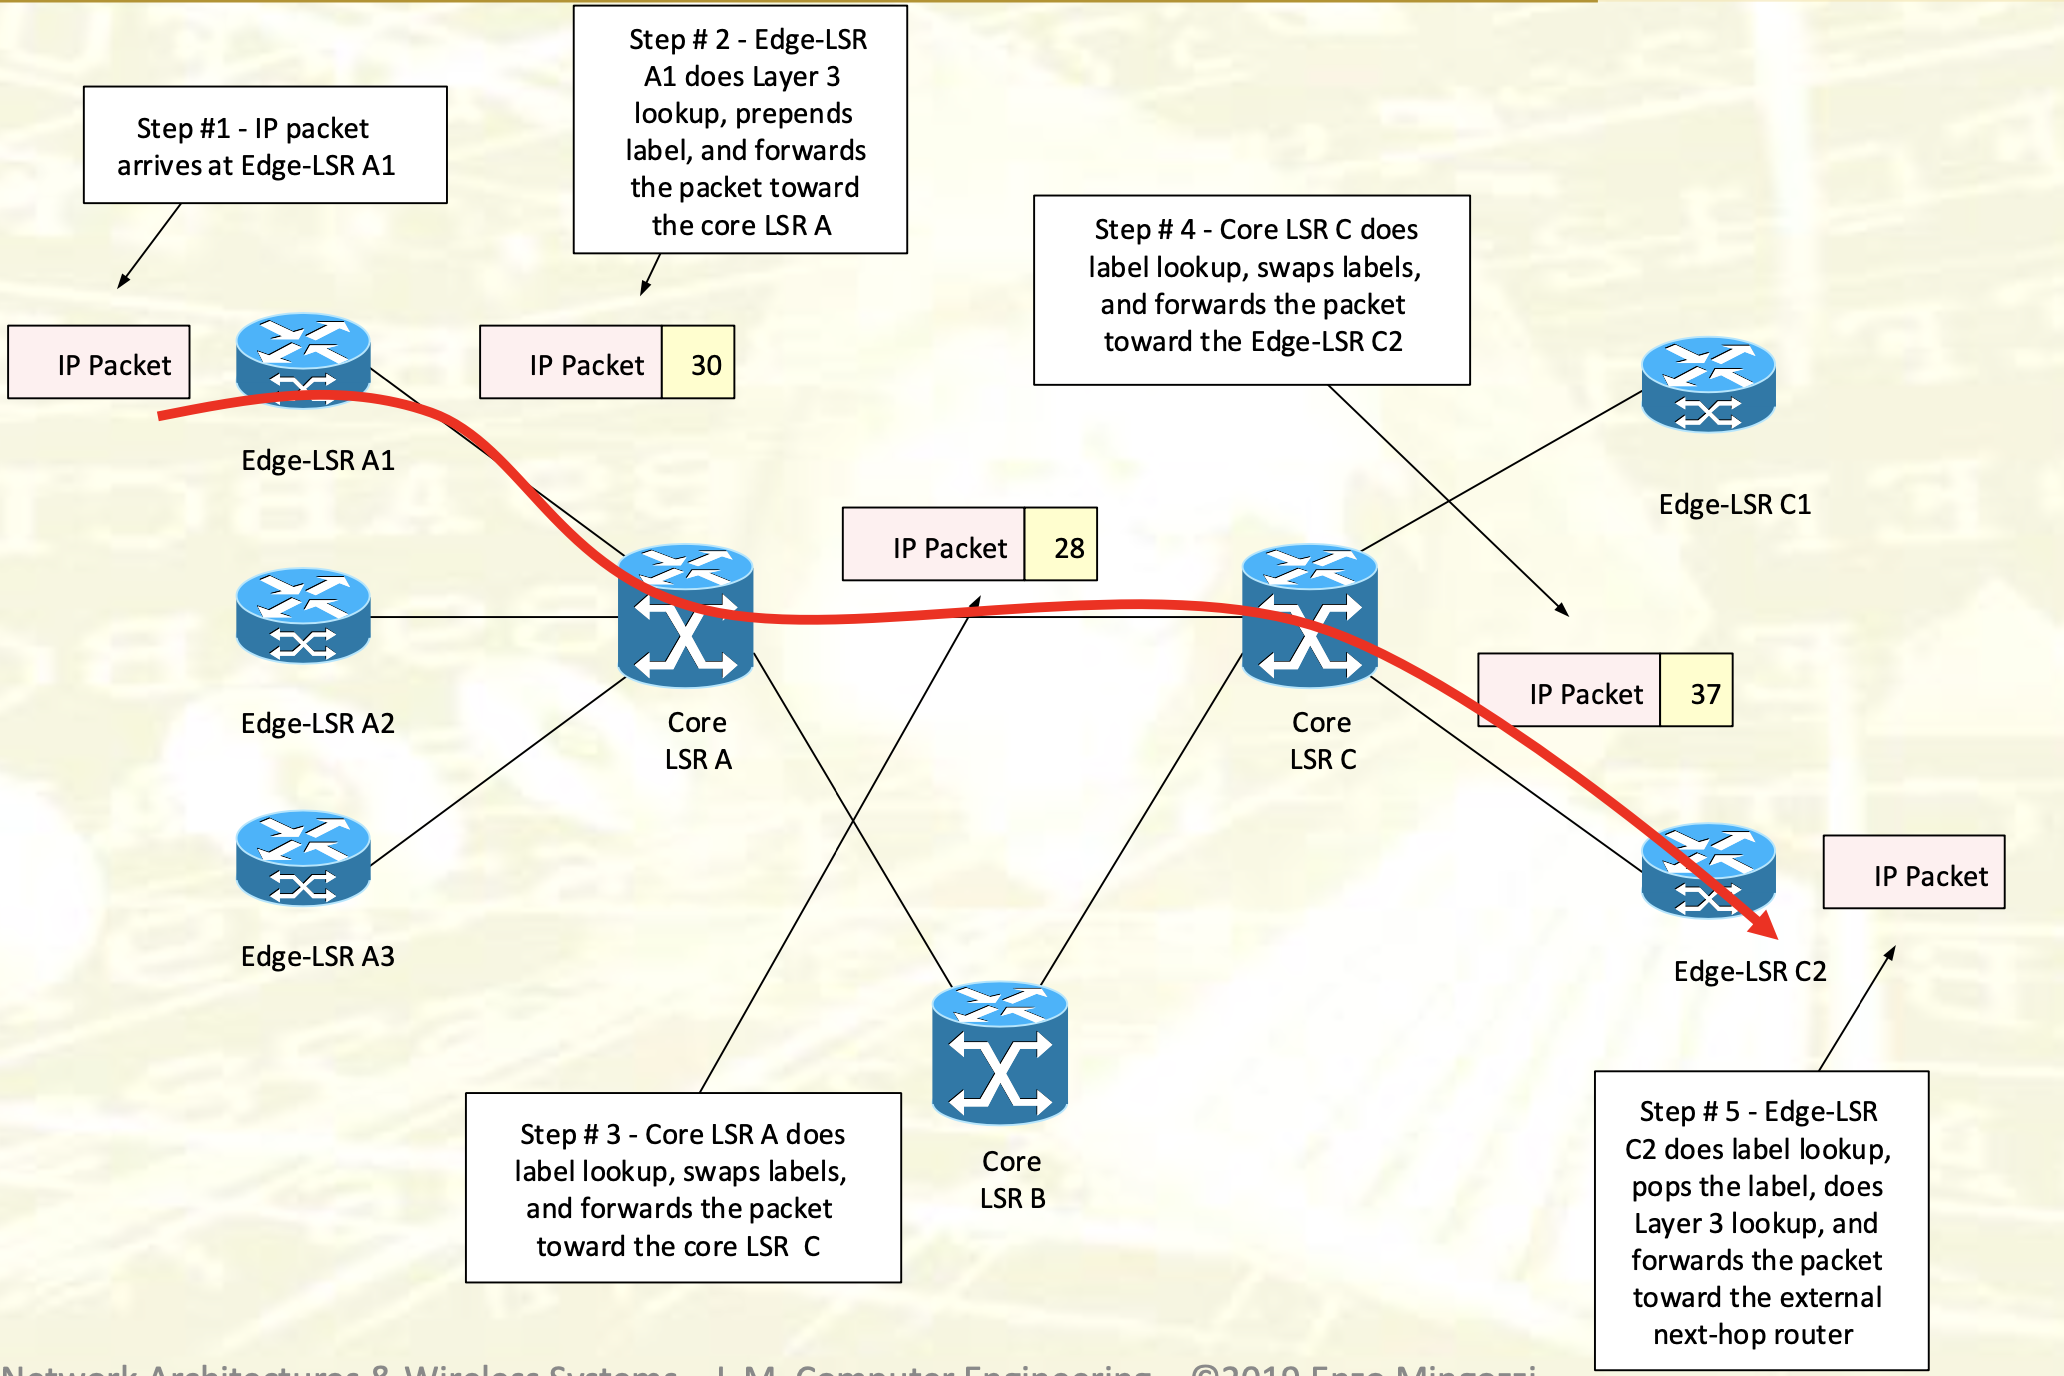
\includegraphics[scale=0.3]{figures/lsp path.png}
    \caption{Label Switched Path}
\end{figure}
\subparagraph{Penultimate Hop Popping (PHP)} Una piccola ottimizzazione può essere effettuata tramite PHP. Considerando cosa accade quando un pacchetto raggiunge l'ultimo hop di LSP: l'ultimo router fa un look up nella sua tabella interna e scopre che deve fare un POP del label: \textit{LFIB: rimuovi il label}. Dopo questa operazione, il router utilizza la routing table IP per effettuare il routing come farebbe normalmente: \textit{FIB: forward del pacchetto IP sulla base dell'indirizzo del prossimo hop}. Quindi, normalmente, si fanno 2 look-ups su tabelle diverse. L'ottimizzazione proposta da questo approccio, consente di fare una sola look-up. Come suggerisce il nome, quindi, si effettua l'operazione di POP non all'ultimo nodo, ma al penultimo. Quindi, il penultimo router effettua la POP ed invia il pacchetto al next hop senza l'etichetta.

\subparagraph{Label Stacking} I concetti espressi precedentemente, sono validi quando è presente un solo label nel pacchetto. Come già detto, è consentito avere più label e questi saranno organizzati a stack (pila). Quindi un pacchetto etichettato, porterà un numero di etichette $m \geq 0$. \\ In questo stack, i pacchetti saranno organizzati in "last-in, first-out", il label 1 è considerato l'ultimo e l'm-esimo il top. Quindi, le azioni nella NHLFE si applicano sempre al top del label nello stack.
\begin{figure}[H]
    \centering
    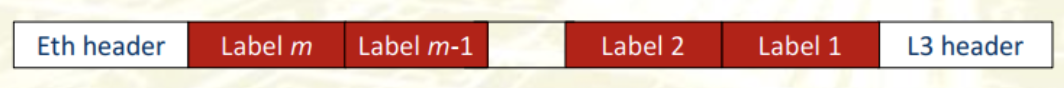
\includegraphics[scale=0.4]{figures/organizzazione header stack.png}
    \caption{Organizzazione degli header con stack}
\end{figure}
Operazioni possibili su uno stack:
\begin{itemize}
    \item \textbf{SWAP Lx:} sostituisce l'etichetta al top dello stack con uno specificato label Lx. Non è possibile fare uno swapping di un'etichetta non in cima alla pila.
    \item \textbf{POP:} effettua l'operazione di POP sullo stack. Come nel caso precedente, non è possibile effettuare questa operazione in un'etichetta non in cima alla pila.
    \item \textbf{PUSH Lx:} effettua l'operazione di push con il nuovo label Lx nello stack. Sono ammesse push multiple. Questa operazione è un po' più elaborata, dato che è un'azione combinata di SWAP e PUSH. Quando arriva un pacchetto nel dominio e devo fare una push dell'etichetta m, faccio sempre una swap all'etichetta m-1, e poi faccio una push dell'etichetta m. Nel caso il pacchetto non abbia altre etichette, viene fatta solo la push senza la swap.
\end{itemize}
L'utilizzo di etichette multiple organizzate in stack, può essere utile per effettuare il tunneling delle LSP.
\begin{figure}[H]
    \centering
    \includegraphics[scale=0.4]{figures/organizzazione header stack.png}
    \caption{Organizzazione degli header con stack}
\end{figure}
L'esempio seguente mostra l'utilizzo delle etichette per creare una sorta di gerarchia di LSP e come vengono gestite le 3 operazioni (swap, pop, push). 
\begin{figure}[H]
    \centering
    \includegraphics[scale=0.3]{figures/tunneling example mpls.png}
    \caption{Esempio di LSP tunneling}
\end{figure}
L'etichetta prima di entrare nel dominio era 30, quando arriva al dominio diventa 28 (viene fatto lo swap) e poi successivamente viene fatta la push dell'etichetta relativa al dominio in cui siamo appena entrati (con label 6). Nel percorso all'interno del domain, l'etichetta con label 28 rimane invariata, viene usato il meccanismo del PHP. Quando si arriva all'ultimo router del dominio, viene fatta la POP della label del dominio, e poi la SWAP della label esterna da 28 a 40. Prima di fare la push, ho bisogno di fare la swap, dato che la label 30 ha valore solo per il router R2, mentre per il router R3 quella classe non corrisponde al label 30, ma al 28. Quindi è necessario che R2 faccia la swap.

\paragraph{Piano controllo MPLS} Con il Control Plane un LSR ha a disposizione delle procedure per: 
\begin{itemize}
    \item creare bindings tra labels e FEC
    \item informare gli altri LSR dei bindings effettuati
    \item costruire e mantenere le strutture dati del data plane
\end{itemize}
\paragraph{LSR label scope} L'associazione tra label e FEC è un'associazione locale: due LSR vicini utilizzeranno il medesimo label per lo scambio dei pacchetti appartenenti alla stessa FEC, dopodiché ognuno dei due utilizzerà un diverso label per i pacchetti appartenenti alla stessa FEC, ma destinati ad altri LSR. \\ Non è detto che una label corrisponda ad una sola FEC:
\begin{itemize}
    \item \textbf{per-platform label space:} dato un LSR  R\textsubscript{D} questo può: associare L\textsubscript{1} ad una FEC F e distribuirla ad un LSR R\textsubscript{U1} oppure associare L\textsubscript{2} ad una FEC F e distribuirla ad un LSR R\textsubscript{U2}.
    \item \textbf{per-interface label space:} dato un LSR  R\textsubscript{D} questo può: associare L\textsubscript{1} ad una FEC F e distribuirla ad un LSR R\textsubscript{U1} oppure associare L\textsubscript{2} ad una FEC F e distribuirla ad un LSR R\textsubscript{U2}. Se e solo se R\textsubscript{D} può determinare la provenienza da R\textsubscript{U1} o R\textsubscript{U2} di un pacchetto con label L, dunque solitamente se valgono entrambe le seguenti: R\textsubscript{U1} e R\textsubscript{U2} sono connessi mediante una connessione punto punto a R\textsubscript{D} e R\textsubscript{U1} e R\textsubscript{U2} sono gli unici peers con cui R\textsubscript{D} scambia informazioni di binding che riguardano L.
\end{itemize}

\subparagraph{Assegnamento ed Allocazione dei Labels} L'assegnamento dei labels è downstream based: sono quindi i downstream LSR a comunicare agli upstream LSR quale label assegnare ad una data FEC. Questo è fatto per evitare la non univocità con peers che fanno uso di un per-interface label space. Quel che può variare è l'allocazione dei label, ossia quando il downstream decide l'associazione label-FEC.

\subparagraph{Downstream On Demand} Con questa modalità un downstream LSR alloca un label ad una FEC solo su richiesta da parte di un upstream LSR. Tale associazione ha valenza solo per una specifica interfaccia.
\begin{figure}[H]
    \centering
    \includegraphics[scale=0.3]{figures/downstream on demand.png}
    \caption{Downstream on demand}
\end{figure}

\subparagraph{Unsolicited Downstream} Con questa modalità un downstream LSR alloca spontaneamente un label ad una FEC ed invia tale associazione a tutti gli upstream LSR adiacenti, non c'è bisogno di alcuna richiesta esplicita.
\begin{figure}[H]
    \centering
    \includegraphics[scale=0.3]{figures/unsolicited downstream.png}
    \caption{Unsolicited Downstream}
\end{figure}
Non è detto, però, che tutti i vicini siano interessati a tale binding, legato all'utilizzo di quel router come downstream LSR per una comunicazione verso la FEC di cui fa advertisement. Si configurano quindi 2 possibilità:
\begin{itemize}
    \item tenere comunque traccia dell'associazione per usi futuri, nel qual caso si parla di \textit{liberal label retention mode}. Tale approccio è consigliato se si vuole avere una reattività ai cambiamenti nel routing, ad esempio per avere sempre a disposizione una backup route nel caso del fallimento di un link.
    \item scartare il binding non tenendone di conto, nel qual caso si parla di \textit{conservative label retention mode}. Tale approccio è consigliato se il problema del salvataggio delle informazioni è piuttosto sentito.
\end{itemize}

\subparagraph{LSP setup control} I bindings FEC-to-label sono distribuiti solo con l'intento di stabilire cammini label-switched. Si creano quindi 2 differenti modalità che rispondono sostanzialmente a due domande: quale FEC utilizzare per avvertire di un binding? La scelta di una FEC determina quale LSP sono costruiti. Quando avvertire questi binding? Questo determina chi ha il controllo sul setup della LSP.

\subparagraph{Ordered Control} Con questa modalità, un LSR effettua un binding tra FEC e label solamente se è un egress router per quella FEC e ha già ricevuto un'informazione di binding per quella FEC. \\
Con la \textbf{Unsolicited Downstream}, l'approccio è il seguente: 
\begin{figure}[H]
    \centering
    \includegraphics[scale=0.4]{figures/ordered control unsolicited downstream.png}
    \caption{Ordered Control - Unsolicited Downstream}
\end{figure}
\begin{itemize}
    \item Il setup del cammino parte dall'egress router che costituirà l'ultimo hop di LSP.
    \item Questo router inizia a fare un broadcasting di messaggi di binding ai suoi vicini per un certo FEC, seguendo un approccio unsolicited downstream.
    \item Ogni altro router, appena ricevuto un messaggio di binding da un router downstream, utilizza la routing table L3 per scegliere quale binding usare e quale router selezionare come hop successivo. Una volta completata la scelta, genere la NHLFE e inizia a fare broadcasting del suo binding ai suoi vicini.
    \item Il processo prosegue fino al router ingress da cui il traffico sarà "iniettato" e il cammino viene così formato.
\end{itemize}
Con la \textbf{Downstream On-Demand}, si ha il seguente approccio:
\begin{figure}[H]
    \centering
    \includegraphics[scale=0.4]{figures/ordered control downstream on-demand.png}
    \caption{Ordered Control - Downstream On-demand}
\end{figure}
\begin{itemize}
    \item Il setup del cammino inizia dal router ingress da cui il traffico è iniettato, appena ha bisogno di scoprire il cammino per un dato FEC.
    \item Utilizzando le tabelle di routing L3, determina il prossimo hop per quello specifico FEC; poi al prossimo hop che binding vuole usare per quel FEC, seguendo un approccio downstream on-demand.
    \item Quando riceve la richiesta con le informazioni di binging dal router upstream, il router downstream, a sua volta, ha bisogno di trovare un cammino per il suddetto FEC. Quindi, a sua volta, determina il prossimo hop dalla sua tabella di routing L3 e gli chiede che binding vuole utilizzare per questo FEC.
    \item Il processo è ripetuto per tutti i router fino a raggiungere il router egress, che costituirà l'hop finale di LSP. Questo router sa come raggiungere la destinazione finale, seleziona un label per la FEC e comunica il binding al router upstream che lo ha richiesto precedentemente.
    \item A questo punto l'ultimo router, a sua volta, decide un binding e lo comunica al router upstream e così via, fino al router iniziale: il cammino è finalmente costruito.
\end{itemize}
Si osserva, quindi, come l'Ordered Control associato all'Unsolicited Downstream: generi un reverse tree e fornisca aggregazione. \\ Mentre, l'Ordered Control associato ad un Downstream On Demand generi un LSP per ogni ingress router.

\subparagraph{Indipendent Control}
In questo caso, c'è soltanto il metodo \textbf{Unsolicited Downstream}:
\begin{figure}[H]
    \centering
    \includegraphics[scale=0.3]{figures/indipendent control.png}
    \caption{Indipendent Control - Unsolicited Downstream}
\end{figure}
\begin{itemize}
    \item Ogni router crea e distribuisce i suoi binding indipendentemente.
    \item All'inizio, quando non c'è ancora nessun binding, un FEC è associato ad un'azione POP e l'indirizzo del prossimo hop, è l'indirizzo di loopback. In questo modo, il label MPLS di un pacchetto è rimosso e il pacchetto è passato al livello 3.
    \item Quando il router downstream decide quale binding usare e lo comunica al router upstream, quest'ultimo cambia l'azione POP con una SWAP del label deciso dal router downstream e setta il downstream come prossimo hop.
\end{itemize}
Dovendo confrontare Indipendent Control ed Ordered Control, possiamo asserire che il secondo fornisce una prevenzione dai loops, ma ha come svantaggio la necessità che i bindings si propaghino per tutta la rete prima che si possa stabilire un LSP. 
\\
Si aggiunge anche una nota che riguarda il modo in cui i router vengono a sapere che sono il penultimo hop e che quindi possono effettuare il PHP. L'ultimo router lo dice esplicitamente, questo è fatto imponendo all'ultimo router di utilizzare un label invertito per il binding. Questo label numero 3, detto \textit{null label}, ogni volta che un upstream router riceve un binding per il label 3, significa che il prossimo router è l'ultimo nell'LSP. 

\subparagraph{Aggregazione (MP2P)} È possibile trattare l'unione di più FEC a sua volta come una FEC, ciò risulta utile quando dei LSP condividono lunghi tratti di percorso. In tal caso le N FEC sono dette aggregabili e su di esse si può agire in 3 modi:
\begin{itemize}
    \item Aggregarle in un'unica FEC.
    \item Aggregarle in un insieme di M FEC (con M $<$ N).
    \item Non aggregarle
\end{itemize}
Se si effettua aggregazione, non si hanno solo risvolti positivi nel processo di forwarding, che si troverà a dover operare con tabelle di dimensioni minori, ma si otterrà anche un ulteriore alleggerimento del processo di distribuzione dei label. Si ha quindi la possibilità di scegliere un livello di granularità compreso fra 2 estremi: \textit{coarset granularity} (aggregazione massima) e \textit{finest granularity} (nessuna aggregazione). Si osservi che: se si utilizza l'ordered control, ogni LSR deve usare la granularità del next hop e se si utilizza l'indipendent control, ogni LSR può usare la granularità che desidera.

\subsubsection{Label Distribution Protocol (LDP)} 
Progettato specificatamente per la distribuzione dei label. Si basa su IGP (Interior Gateway Protocol, il protocollo utilizzato all'interno di un sistema autonomo, ad esempio OSPF), per tutte le decisioni relative al routing. LSR A che riceve un mapping per il label L per il FEC F, dal suo peer LDP; LSR B utilizzerà il label L per il forwarding se e solo se B è bel cammino minimo IGB per la destinazione F dal punto di vista di A. \\ Maggiori funzionalità:
\begin{itemize}
    \item Discovery dei vicini (UDP)
    \item Creazione e mantenimento della sessione (TCP)
    \item Advertisement del label
    \item Notifiche
\end{itemize}

\subsection{}{RSVP per la distribuzione dei label} Resource Reservation Protocol. È stato definito per QoS, ma è stato esteso per la distribuzione dei label. 
\begin{figure}[H]
    \centering
    \includegraphics[scale=0.4]{figures/RSVP label distribution.png}
    \caption{RSVP for label distribution}
\end{figure}
Ci sono 2 tipi di messaggi: PATH message e Reservation (RESV) message. I messaggi PATH viaggiano dall'upstream al downstream (from HEAD-END a TAIL-END) in un dominio e propagano l'info riguardante la FEC che si vuole stabilire. I messaggi RESV viaggiano poi all'indietro sullo stesso cammino, seguiti da messaggi di path che forniscono informazioni riguardo i binding dei label. \\ Il protocollo garantisce che RESV seguano esattamente il cammino dei PATH.

\subsection{LSP setup control} Quale FEC si utilizza per fare l'advertising di un binding? \\ Quando si fa l'advertising del binding?
\begin{itemize}
    \item \textbf{Ordered control:} Egress (o ingress) LSR hanno il controllo su quale LSP devono fare setup. Il comportamento di default è che la FEC mappi l'indirizzo edge LSR loopback.
    \item \textbf{Indipendent control:} Tutti i router fanno l'advertising della FEC indipendentemente (ma devono farlo in una modalità consistente). Il comportamento di default è che si mappi ogni FEC per tutti i prefissi della tabella di routing.
\end{itemize}
Si considera adesso una destinazione del network nella tabella di routing IP (1 network prefix), questo ha una corrispondenza stretta con una certa FEC. In tutti i network si va a definire una corrispondenza tra una FEC e un edge router. Se ho un dominio di transito (questo funziona per pacchetti entranti nel network e trova un cammino all'interno di questo stesso network in modo da trovare un'uscita da quest'ultimo), dato che il numero di router (egress e ingress) sono tipicamente un subset ridotto rispetto a tutti gli altri, l'unica informazione di cui abbiamo bisogno è di conoscere il cammino da usare per raggiungere l'edge router in modo da uscire dal dominio. \\ Invece di avere una entry per ogni network, potremmo avere, all'inizio, una entry per ogni router edge. \\ Se ad esempio consideriamo OSPF, ogni nodo conosce l'ID del router edge e conosce il modo di raggiungerlo. Se il primo router (R1), quando arriva un pacchetto, con indirizzo di destinazione 10.1.1.1, utilizza il database OSPF e sa che questo è esterno a questo sistema autonomo, controlla quale sia l'edge router da usare per questo indirizzo. Da qui, la corrispondenza tra LSP ed edge router. \\ Questo è un pezzo di informazione che è condiviso tra tutti i router, si aggregga tutto il traffico che sta andando all'esterno del dominio attraverso uno specifico LSR. In ogni caso, tutti i pacchetti seguono esattamente lo stesso cammino che seguirebbero con IP. Non stiamo cambiando come i cammini sono calcolati e non c'è nessun controllo sul cammino.

\subsection{Supporto MPLS per DiffServ} MPLS è una soluzione per fare il forwarding dei pacchetti IP alla loro destinazione, questo è per prendere decisioni riguardo il prossimo hop. \\ DiffServ è un'architettura network e soluzione di molti problemi, indipendentemente dalle funzioni di forwarding. MPLS è relativo al data plain, ma anche il per hop behaviour è relativo al data plain. MPLS ha il suo header, QoS utilizza quello di IP (campo DSCP per scegliere PHB). Vorremmo un sistema per evitare di doverlo consultare. \\ Nell'header MPLS, ci sono 3 bit per il traffic class (TC), quindi si va ad utilizzare questo campo, se ci sono soltanto 8 PHB nel dominio (si codificano i 6 bit di DSCP in questi 3). \\ Che succede se ho più di 8 PHB? Si utilizza lo stesso label: il label indica il prossimo hop e TC come gestire il pacchetto. Quindi si configurano 2 casi:
\begin{itemize}
    \item Caso fortunato: PHB $<$ 8: Posso utilizzare TC. Quando un pacchetto arriva ad un router, si fa il lookup del label per identificare il prossimo hop, si controlla TC per capire il PHB. Per esempio, quando il label $=$ 001, il router sa che è assicurata la classe di forwarding 1 e quindi tratterà il pacchetto di conseguenza.
    \item Se abbiamo più di 8 PHB, dobbiamo usare i label anche per distinguere i PHB
\end{itemize}
Al fine di supportare DiffServ, è necessario che gli LSR possano desumere il PHB da applicare ad un determinato pacchetto appartenente ad un BA (Behaviour Aggregate) esaminando il solo header. \\ Esistono 2 modalità, il cui impiego è condizionato dal numero di PHB supportati dalla rete: 
\begin{itemize}
    \item \textbf{E-LSP:} il PHB viene desunto osservando il solo campo EXP (CoS) nello shim header. Non richiede modifiche alle operazioni di signaling.
    \item \textbf{L-LSP:} il PHB viene desunto osservando i campi label ed eventualmente EXP dello shim header. Richiede modifiche alle operazioni di signaling.
\end{itemize}
\paragraph{E-LSP} Qualora siano implementati nel dominio DiffServ/MPLS, solamente 8 PHB, si può utilizzare la modalità \textit{Experimental LSP}. Infatti, nell'architettura DiffServ, il PHB da applicare ad un determinato BA viene deciso ad un router DiffServ mediante l'analisi DSCP all'interno del campo DS: esso è un valore a 6 bit. \\ In tale implementazione, invece, si riservano solamente 3 bit (del campo Exp) avendo quindi uno spazio di possibili PHB ridotto. Quindi, potrebbero non bastare se i PHB da implementare sono più di 8. \\ Il pregio di tale soluzione risiede nel fatto che non sono necessari ulteriori meccanismi di signaling: il protocollo di Label Distribution lavora come di consueto; durante le operazioni di forwarding, gli LSR desumono all'interno dello shim header: il PHB da applicare ad un pacchetto consultando il campo Exp e dove effettuare il forwarding mediante il campo label. \\ Si necessita solamente di una preventiva configurazione: così come i PHB venivano mappati su un DSCP, adesso vengono mappati sul campo Exp.
\begin{figure}[H]
    \centering
    \includegraphics[scale=0.4]{figures/exp lsp.png}
    \caption{EXP-Inferred LSP}
\end{figure}
\paragraph{L-LSP} Qualora siano implementati nel dominio DiffServ/MPLS più di 8 PHB, si può utilizzare la modalità \textit{Label LSP}. Il PHB da applicare viene dunque inferito dal label del pacchetto, si necessita quindi di un enhancement del meccanismo di label distribution. Il protocollo LDP deve essere esteso affinché i messaggi che richiedano o comunichino il binding per una determinata FEC, includano anche le informazioni sul PHB ad essa associato. \\ Per quanto riguarda il gruppo PHB AF, i pacchetti che condividono un PHB comune vengono riferiti come appartenenti alla medesima PHB scheduling class: essi percorreranno il medesimo LSP in MPLS e la relativa drop precedence è indicata all'interno dei 3 bit del campo Exp. Questo nel frame mode, mentre nel cell mode si utilizza il campo CLP dell'header della cella. \\ Per tutti gli altri PHB, ogni LSP trasporterà pacchetti appartenenti ad un singolo PHB. In tali casi, i bit del campo Exp non sono utilizzati. 
\begin{figure}[H]
    \centering
    \includegraphics[scale=0.4]{figures/labelonly lsp.png}
    \caption{Label-Only-Inferred LSP}
\end{figure}

\newpage
\section{Traffic Engineering}
Vogliamo controllare il percorso seguito dal traffico attraverso una rete in modo tale da massimizzare l'utilizzazione di tutti i link cercando, allo stesso tempo, di evitare la congestione della rete. Evitare la congestione significa diminuire le perdite di pacchetti e quindi aumentare l'utilizzo della rete. Per fare ciò abbiamo bisogno di avere il controllo esplicito sul traffico: vogliamo sapere ingresso e uscita dalla rete, decidere il percorso che quello specifico flusso deve seguire ecc. Questo non si può fare con IP classico.\\
Abbiamo bisogno di algoritmi di routing \textit{constraint-based}, ovvero degli algoritmi e protocolli che minimizzano il costo (secondo una metrica scalare) e che tengano anche conto di determinati vincoli. Alcuni esempi di vincoli sono:
\begin{itemize}
    \item Performance: trovare un percorso con una certa banda minima disponibile.
    \item Amministrativi: possibilità di escludere determinati link per questioni amministrative.
\end{itemize}
Si può anche avere una combinazione di vincoli.\\

\subsection{Link Characterization}
Se vogliamo modificare un protocollo di routing esistente (tipo OSPF) per supportare il Traffic Engineering, ci servirnno ulteriori informazioni oltre al costo dei vari link. Alcuni dei nuovi parametri sono:
\begin{itemize}
    \item Max Badwidth: la capacità del link.
    \item Max reservable Bandwidth: la quantità riservabile di un link.
    \item Unreserved Bandwidth: banda ancora disponibile su un link.
    \item Administrative Group: indica un "gruppo" a cui un link appartiene. In questo modo si può discriminare i vari link se non si voglio attraversare.
\end{itemize}
Gli attributi dei link dovranno quindi essere diffusi come parte delle informazioni di routing dal protocollo di routing. OSPF-TE è la versione estesa di OSPF per supportare il Traffic Engineering. Ogni router è a conoscenza degli attributi correnti di tutti i link in una determinata area. Questi dati vengono salvati nel Traffic Engineering Database (TED).\\
Lo scambio di queste informazioni può essere periodico oppure in risposta ad eventi (cambiamenti dello stato dei link). Tuttavia, se i cambiamenti dei link diventano frequenti, si rischia di sovraccaricare la rete con messaggi di controllo. In questi casi è più opportuno usare un approccio periodico, anche se meno preciso sarà comunque più scalabile.\\
In OSPF-TE ci sono alcuni attributi che sono statici mentre l'attributo \textit{unreserved bandwidth} cambia frequentemente perché varia ogni qualvolta un flusso riserva della banda. Per questo motivo l'approccio event-based non è scalabile e, in partica, si utilizza un approccio ibrido.

\subsection{Protocolli di Routing Estesi}
\subsubsection{CSPF}
E' una versione dell'algoritmo di Dijkstra (SPF) estesa per il TE in cui abbiamo i vincoli (Constraint SPF). Inizialmente applichiamo i vincoli a tutti i link nel TED, dopodiché applichiamo l'algoritmo di Dijkstra (SPF) per calcolare il grafo dei percorsi minimi. SPF viene calcolato a partire dal router d'ingresso della rete perchè quest'ultimo conosce la topologia.

\subsubsection{RSVP-TE}
Algoritmo che serve per permettere a nuovi flussi di riservare le risorse e allo stesso tempo costruire un percorso. RSVP viene esteso per supportare LSP dopo che è stato ottenuto il grafo dei percorsi minimi tramite CSPF. Il pacchetto contiene la lista dei router da attraversare.\\
L'ingress router dell'LSP che vogliamo costruire si chiama \textit{head-end} ed ha il compito di iniziare il protocollo mandando un \textit{Path-message} al quale riceverà, come risposta, una \textit{Resv-message}. La differenza rispetto a RSPV tradizionale è che questi due messaggi trasportano informazioni aggiuntive. In particolare, per il path-message abbiamo:
\begin{itemize}
    \item Label Request Object (LRO): indica che vogliamo creare un percorso e fare label binding ad ogni hop.
    \item Explicit Route Object (ERO): contiene il percorso da seguire in termini di hops. Questo percorso può essere calcolato direttamente dallo \textit{head-end} in modo da evitare computazioni ad ogni hop. Esiste un bit all'interno dell'ERO che indica se gli hops contenuti sono \textit{strict} o \textit{loose}. Nel primo caso i nodi adiacenti sono direttamente connessi e quindi il percorso sarà esattamente quello descritto dall'ERO. Nel secondo caso lo \textit{head-end} può fornire una lista di nodi tale che due nodi successivi possano non essere direttamente connessi. In questo caso ogni nodo del percorso può calcolare il percorso del next node della lista in maniera autonoma usando CSPF.
    \item Record Route Object (RRO): contiene lo stato relativo a questa operazione.
    \item Sender TSpec: contiene la traffic demand.
\end{itemize}
Per il resv-message abbiamo:
\begin{itemize}
    \item Record Route Object (RRO)
    \item Label Object: specifica la label scelta da un router per questo LSP che deve essere comunicata al router soprastante (upstream) nel percorso.
\end{itemize}
Per evitare situazioni di conflitto sulle risorse, esiste l'Admission Control su ogni hop. Quando un percorso scelto trmaite CSPF viene scelto, gli viene garantito che ci siano abbastanza risorse lungo il percorso. Questo nella realtà non è sempre vero in quanto le informazioni contenute nella TED potrebbero non essere aggiornate.\\
Le LSP forniscono 8 livelli di priorità. In realtà si utilizzano solo 2 priorità:
\begin{itemize}
    \item \textbf{setup priority:} per percorsi in costruzione.
    \item \textbf{hold priority:} per percorsi che sono già attivi.
\end{itemize}
Se due flussi vogliono riservare delle risorse contemporaneamente, ma non ci sono abbastanza risorse per entrambi, la setup priority è usata per discriminare quale dei due sarà accettato.\\
Poichè le condizioni della rete cambiano in maniera dinamica, il percorso ottimale per un flusso potrebbe cambiare nel tempo. Per questo motivo è necessario ri-eseguire CSPF in modo tale da aggiornare le LSP. Questo processo è chiamato ri-ottimizzazione.

\subsubsection{Fast Re-Routing}
Esempio di applicazione di MPLS-TE. In caso di fallimenti di rete, nelle reti tradizionali quello che succede è che l'elemento che ha rilevato il problema informa tutti gli altri che, a loro volta, ri-calcoleranno i percorsi. Il problema di questo approccio è che impiega molto tempo.\\
Grazie a fast re-routing si può trovare un percorso alternativo e temporaneo per sopperire (seppur parzialmente) al malfunzionamento della rete fino a che non verrà calcolato un nuovo percorso ufficiale. Tutto questo viene realizzato avendo un LSP di backup pre-calcolato per ogni link: quando viene rilevato un fallimento, l'LSP di backup viene usato immediatamente sfruttando il tunneling MPLS per bypassare il link che è fallito.

\newpage
\section{BGP - Border Gateway Protocol}
L'architettura attuale di Internet prevede diverse autorità che controllano differenti porzioni della rete in modo indipendente (Autonomous Systems). Data questa struttura complessa con differenti blocchi autonomi, il nostro obiettivo è, dato un pacchetto con indirizzo di destinazione, trovare un metodo per inviare quel pacchetto al dominio (AS) che contiene l'indirizzo destinazione. Si può ottenere tramite BGP.
\begin{figure}[H]
    \centering
    \includegraphics[scale=0.5]{figures/internet_architecture.jpg}
    \caption{Architettura di Internet con AS}
\end{figure}
BGP è un'istanza dell'algoritmo \textit{Path Vector Routing}. Non è un algoritmo di tipo link-state né di tipo distance-vector in quanto:
\begin{itemize}
    \item (link-state) costruire la topologia dell'Internet globale ad ogni nodo e calcolare il percorso minimo è una soluzione non-scalabile.
    \item (distance-vector) c'è una buona probabilità che emergano cicli che sarebbero pericolosi in una topologia così grande.
\end{itemize}
In BGP consideriamo ogni AS come un nodo della rete, che può essere collegato ad altri AS tramite archi (link che collegano i border-router). Quello che vogliamo trovare è quindi il "next-hop" che in questo caso sarà il next-AS del percorso.\\
Ogni nodo AS scambia con i suoi vicini dei messaggi che contengono una destinazione nota e la lista di nodi (AS) che formano il miglior percorso conosciuto verso quella destinazione. Questo è una differenza importante rispetto al distance-vector perché aiuta a prevenire i cicli: se un nodo \(x\) riceve un \textit{path-vector} in cui \(x\) stesso è incluso, il messaggio deve essere scartato altrimenti si forma un ciclo.\\
Il costo di ogni hop è sempre pari ad 1 anche se, tramite un trucco, è possibile aumentarlo: basta ripetere l'id di un nodo più volte nel percorso. In questo caso si parla di \textit{path manipulation}.\\
Queste idee vengono messe in pratica nel protocollo BGP-4. I nodi (AS) della rete non s parlano direttamente bensì sono i border router (BR) a scambiarsi tutti i messaggi tramite una connessione TCP. Possiamo avere più BGP peers (border-router che scambiano messaggi BGP) all'interno di uno stesso AS oppure in due AS diversi:
\begin{itemize}
    \item \textbf{E-BGP (esterni):} i due BR appartengono ad AS diversi.
    \item \textbf{I-BGP (interni):} i due BR appartengono allo stesso AS. Questo serve perché i BR potrebbero essere connessi a due AS diversi pertanto, ci sarà necessità di scambiarsi i differenti pezzi di informazione raccolti.
\end{itemize}
Fra i vari messaggi BGP che si scambiano i router, di particolare interesse sono gli UPDATE, scambiati periodicamente. Un messaggio di tipo BGP-UPDATE contiene una lista di \textit{Path Attributes} che codificano le informazioni che rappresentano un percorso verso una certa destinazione. Alcuni di questi attributi sono:
\begin{itemize}
    \item ORIGIN: da dove è partito il messaggio.
    \item AS\_PATH: lista di ID degli AS che compongono il percorso verso la destinazione.
    \item NEXT\_HOP (next-as).
    \item LOCAL\_PREF: serve in caso vi siano più percorsi verso una destinazione. Grazie a questo campo possiamo impostare una rotta "preferita".
\end{itemize}
Un'altra informazione inclusa nei messaggi BGP-UPDATE è il \textbf{Network Layer Reachability Information} che contiene la lista delle reti raggiungibili tramite il percorso descritto nel campo AS\_PATH.

\newpage
\section{VPN}
Il problema delle cosiddette "Corporate WANs" consiste nel voler collegare fra loro delle reti che si trovano molto distanti l'una dall'altra. Vogliamo che il collegamento le faccia risultare vicine. Il problema è che, essendo distanti, non esiste un collegamento diretto fra queste reti pertanto, sarà necessario implementare un meccanismo che simuli la "vicinanza". \\ Tale rete non potrà essere pubblica, ma privata, ovvero deve essere utilizzabile solo dalla compagnia e deve avere un meccanismo di routing ed uno spazio degli indirizzi indipendenti dal resto delle reti con cui condivide l'infrastruttura mediante la quale è realizzata.
\subsection{Concetti generali}
\paragraph{Overlay VPN} In questo modello, ogni sito ha un router che è connesso mediante un link punto punto virtuale ad altri routers locati in altri siti. La gestione dell'overlay è fornita dal service provider. In questa connessione punto-punto, i router si scambiano pacchetti del routing protocol in modo da scambiarsi informazioni riguardo la network reachability. Questo si può fare a più livelli: stendendo linee fisiche (livello 1, anche se in questo caso non si tratterebbe più di rete virtuale), oppure al livello 2 (con, ad esempio, una tecnologia Frame Relay, packet switched). Questo tunneling può essere fatto anche al livello 3 (IP over IP tunneling, usando protocolli come Generic Route Encapsulation o IPsec). \\ Si ottengono risultati sperati, ovvero: connettività tra i siti, indirizzi privati (no vincoli nell'addressing) e traffico privato. Si ottengono tuttavia degli svantaggi da questo approccio. I Customer Edge Routers (CE) possono essere gestiti dal cliente, però devono saperli connettere e configurare, cosa non scontata. Problemi di scalabilità: occorre un router per sito, quindi può non essere facile fare manuntenzione della configurazione su decine di migliaia di router, che si trovano in luoghi diversi. Se si deve aggiungere un nuovo sito, su richiesta del cliente, si deve configurare non solo il router appartenente al nuovo sito, ma anche i router precedenti, che devono quindi essere in grado di raggiungere il nuovo sito. È quindi complicato mantenere l'overlay.
\begin{figure}[H]
    \centering
    \includegraphics[scale=0.5]{figures/overlay vpn.png}
    \caption{Overlay VPN}
\end{figure}

\paragraph{Peer-to-peer approach} I peering sono stabiliti fra router CE e solo con il router edge del provider (PE). Quindi, ogni router del customer, scambierà informazioni di routing solo con il provider edge router a cui sono connessi. Quindi, indipendentemente dal numero di "siti" del customer, il numero di peer di ogni customer edge router sarà uno. Ora la configurazione di CE è estremamente semplice: all'esterno del sito del customer, hai un unico next hop possibile. Prima ne avevamo tanti, ovvero quanti il numero di virtual tunnel/virtual link, tramite i quali eri connesso agli altri siti. 
\begin{figure}[H]
    \centering
    \includegraphics[scale=0.5]{figures/peer-to-peer approach.png}
    \caption{Peer-to-peer approach}\label{figura:peer}
\end{figure}
Il problema di questo approccio riguarda la figura \ref{figura:peer}, in cui i colori gialli delle nuvole indicano che appartengono ad altri clienti rispetto a quelli delle nuvole grigie: 5 siti, 2 customer. Questi clienti fanno un addressing indipendente, ci sono degli overlapping. Quindi, i problemi sono: come realizzare private addressing e isolamento del traffico. \\ Una soluzione potrebbe essere quella di inserire dei filtri nei Provider Edge Routers. Un pacchetto originato, ad esempio da 10.2.0.0 "grigio", se è destinato ad un sito "grigio" viene permesso, altrimenti viene filtrato. In pratica, si configura una grande ACL all'interfaccia di ingresso di ogni PER, per controllare se il traffico può entrare nella rete o meno: questo in base al fatto che sia indirizzato ad uno dei siti consentiti o meno (assumendo che si sappia la source). Questa non è una soluzione buona, dato che si considera la network del provider come un "single routing domain", non si possono avere più site con lo stesso indirizzo: si perderebbe così il private addressing oppure, al più, dovremmo implementare delle complicate traduzioni. Si raggiungerebbe comunque un isolamento del traffico, ma ad un costo molto alto, dato che si dovrebbero mantenere dei complessi ACL ad ogni PE. Questa configurazione dovrebbe poi essere continuamente revisionata, dato che ogni volta che cambia la topologia di rete, si devono riconfigurare i PE (le loro ACL). Le ACL, inoltre, rallentano il routing e aggiungono latenza. Quindi, questa soluzione è di difficile applicazione. \\ Cercando un'altra soluzione, l'effetto che si vorrebbe ottenere, è quello che se c'è un pacchetto che va da CE a PE, questo venga consegnato solo se la routing table che è usata per quel pacchetto, che include solo gli indirizzi di destinazione degli altri siti dello stesso customer, sa qual è il next hop di quel pacchetto. Quindi, sempre nella figura \ref{figura:peer}, se consideriamo il site 10.3.0.0/16, appartenente ad un cliente "giallo", se questo manda un pacchetto con destinazione 10.2.0.0/16, ci si aspetterebbe che il PE a cui è attaccato filtri questo pacchetto, in quanto nella rete del cliente giallo, non ci sono sites con tale indirizzo. Come si può ottenere questo effetto? \\ La soluzione è tenere diverse routing table nel PE, una per ogni customer. E' come se si considerassero più router logici, uno per ogni cliente. Si controlla nella tabella giusta, in base al cliente che ti sta inviando quel pacchetto. Questo si chiama \textit{Constrain Routing}, perché i PE si scambiano informazioni, che saranno diverse per diversi clienti, quindi durante lo scambio delle informazioni occorrerà mettere informazioni relative ad un certo cliente, nella sua routing table. C'è ancora un problema di overlapping, quando una rete manda un pacchetto con un indirizzo, presente in 2 clienti diversi, si crea un problema di forwarding per siti con indirizzi in overlapping. La soluzione quindi è quella di utilizzare un tunneling tra provider edge router. È una soluzione standard che troviamo negli RFC, chiamata \textit{BGP/MPLS IP Layer 3 VPN}.

\subsection{BGP/MPLS IP VPN} Considerando lo scenario presente nella seguente figura:
\begin{figure}[H]
    \centering
    \includegraphics[scale=0.5]{figures/bgp-mpls vpn.png}
    \caption{Rete BGP/MPLS IP VPN}\label{figura:bgpmpls}
\end{figure}
Il customer deve solo avere un link al PE e notificare com'è fatta la sua rete. Nella figura \ref{figura:bgpmpls} si ha P che è un Core Router. In ogni Provider Edge Router si hanno diverse tabelle, una per ogni Customer Edge Router connesso. Si distinguono i pacchetti dei diversi clienti in base all'interfaccia sulla quale arrivano. Queste tabelle sono chiamate \textit{Virtual Routing Forwarding Table (VRF)}. Quindi nel PE1, troveremo una VRF per CE1.1 e CE2.1, con questo approccio è come avere molteplici router virtuali, c'è poi una routing table per il global forwarding, ovvero per forwardare traffico non destinato a siti customers. \\ Quindi, se il site1 (grigio), manda un pacchetto all'indirizzo 10.3.1.1, il pacchetto va prima a CE1.1, poi a PE1 che, in base alla interfaccia di provenienza, sa che deve guardare la tabella di routing per il cliente 1. Non troverà un'entrata per 10.3.0.0/16 e quindi scarterà il pacchetto. Come fa PE1 a sapere che, ad esempio, 10.2.0.0/16 può essere raggiunta tramite PE2? Glielo deve dire PE2, occorre un dynamic routing protocol, ovvero PE2 avverte PE1 che quell'indirizzo è raggiungibile attraverso di lui, come fanno i normali protocolli di routing. Tuttavia, adesso si devono scambiare informazioni anche riguardo la proprietà dell'indirizzo, customer giallo o grigio. Questo può essere fatto facendo facendo girare un'istanza del protocollo di routing per VPN. In tal modo è come avere n reti separate, anche se questo approccio non scala, dato che si devono configurare tante istanze di routing protocol per quanti customer si hanno. \\ Si vuole quindi avere una sola istanza del protocollo di routing. In questo caso entra in gioco BGP. 
\begin{figure}[H]
    \centering
    \includegraphics[scale=0.6]{figures/BGP route distribution.png}
    \caption{BGP Route Distribution}
\end{figure}
Tramite un BGP update, PE1 dirà a PE2 quali destinazioni sono raggiungibili tramite di lui, specificando anche il site. Si sta, quindi, informando il PE2 che il PE1 è il next hop per certe destinazioni. Il problema però sorge perché con BGP standard, non si può, nella lista, mettere 2 volte lo stesso indirizzo di destinazione. Non c'è spazio per marcare un indirizzo come "grigio" piuttosto che "giallo". \\ La soluzione risulta quella di definire nuove famiglie di indirizzi VPN-IP: un nuovo schema di indirizzamento, dove aggiungiamo alla destinazion network un prefisso, chiamato \textit{Route Distinguisher (RD)}, di 8 byte che deve essere unico globalmente. 
\begin{figure}[H]
    \centering
    \includegraphics[scale=0.6]{figures/Route distinguisher.png}
    \caption{Route Distinguisher}
\end{figure}
Grazie a questo RD, adesso abbiamo route distinti (per colore) e non si hanno problemi con BGP. \\ Ogni router può usare un RD differente a quello degli altri router per riferirsi a una tabella. Se si usasse RD per ogni VPN, non si avrebbe questo problema, ma si assume che non si stia utilizzando questa soluzione. Quindi, RD non può essere usato come indice nelle VRF, ma viene usato solo per differenziare i messaggi in BGP. \\ Un altro problema è: si vuole più flessibilità, si potrebbe aver bisogno di comunicare tra un host della VPN gialla e uno della grigia. La soluzione a questo problema è raggiunta tramite \textit{Route Target}: è un altro numero, differente da RD. Viene trasportata in un altro attributo di BGP, il \textit{Community Attribute}. Quando arriva un annuncio a un router, per ogni tabella del router viene controllato il Route Tag: se quel Route Target è consentito per quella tabella, allora l'indirizzo viene aggiunto in quella tabella, altrimenti no. 
\begin{figure}[H]
    \centering
    \includegraphics[scale=0.5]{figures/route target.png}
    \caption{Route Target}
\end{figure}
Nelle tabelle si hanno due valori in RT, per import ed export.
\begin{itemize}
    \item \textbf{Import-RT}: specifica quale route vogliamo importare in un dato VRF: se il set di Import-RT include almeno uno degli RT nel messaggio BGP, l'informazione contenuta nel messaggio BGP, è usata per aggiornare la VRF
    \item \textbf{Export-RT}: è la lista di RT che devono essere incluse in un messaggio BGP che annuncia le rotte da questa VRF.
\end{itemize}
Questa modalità di utilizzare Route Target è chiamata \textit{Full-mesh}.
\begin{figure}[H]
    \centering
    \includegraphics[scale=0.5]{figures/full-mesh vpn.png}
    \caption{Full-mesh VPN}
\end{figure}
Adesso, bisogna vedere come inoltrare i pacchetti. Dato che nel mezzo a dei PE, potrebbero esserci delle reti IP, quindi con destination-based forwarding, risulta quindi impossibile proseguire. È necessario fare tunneling tra PE (MPLS tunnel). I router interni scambiano solamente i pacchetti tra i PE, non sanno nulla dei VPN-IP e delle VRF, quindi torna di nuovo il problema dell'overlapping degli IP. Giunto ad un PE, l'informazione "giallo o grigio", non può essere trovata nel pacchetto IP (dato che è presente il tunnel). L'idea è quindi quella di avere più tunnel, uno per VPN. Quindi, se un pacchetto è appartentente alla VPN "gialla", attraverserà l'LSP "giallo". \\ Si può, però, fare di meglio attraverso il label stacking. Si avrà un tunnel tra PE1 e PE2 e si avrà lo stack di multipli LSP su questo tunnel, uno per ogni VPN. 
\begin{figure}[H]
    \centering
    \includegraphics[scale=0.5]{figures/vpn label stacking.png}
    \caption{MPLS label stacking su VPN}
\end{figure}
Lx ed Ly individuano il tunnel tra PE1 e PE2, L2 individua la VPN giusta. Come sapere a chi corrisponde L2? \\ Questa informazione la propaga BGP. Il messaggio BGP contiene RD, RT (per il route filtering), label che indica quale routing table usare. Per aggiungere un nuovo site, con questo approccio, è necessario ritoccare la configurazione del PE a cui si sta connettendo: gli deve comunicare gli RT di import ed export. Queste info vengono poi passate fra i router col protocollo di routing. \\ Come si può linkare una label ad una specifica tabella? Mediante MP-iBGB, il router PE2 indica nel messaggio di MP-iBGP update, quale label deve essere utilizzato come VPN label.

\paragraph{Benefici di BGP/MPLS IP VPN} Per quanto riguarda il customer:
\begin{itemize}
    \item Sbarazzarsi e scaricare la gestione del routing al provider
    \item Avere servizi di regolamento degli accesso (firewall ecc..)
\end{itemize}
Per quanto riguarda il provider:
\begin{itemize}
    \item Serve multipli clienti VPN con una infrastruttura comune
    \item La gestione di VPN è nascosta nel core
    \item Scala aggiungendo PE quando necessario
\end{itemize}
Il tunneling di MPLS gioca un ruolo chiave per consentire tutto questo.
\end{document}